\chapter{METHODOLOGY}
\label{ch:tocloft}

\section{Parametric Curve Interpolation}

This work involves the realtime interpolation of parametric curves with chord-error and feedrate constraints. The steps required are as follows:

\begin{enumerate}
	\item Obtain the mathematical equations of functions describing the parametric curves.
	
	\item Establish the relationship between the parametric curve, chord-error and machine feedrate in CNC terms. 
	
	\item Understand and formulate CNC machine dynamic and kinematic constraints.
	
	\item Develop and execute a realtime algorithm that satisfies chord-error and feedrate constraints when run on the CNC machine.
	
	\item Generate a RS274D NGC G-code for run simulations and offline execution of the algorithm.

\end{enumerate}
  
%% \clearpage
%% \pagebreak

\section{Selection of parametric curves}

\begin{table}[ht]
%% \begin{center}
\caption{List of ten(10) selected parametric curves}
\label{List-of-selected-parametric-curves}
\begin{tabular}{ p{1.00cm} p{11.0cm}}
\hline
	1  & Circle curve\\
	2  & Ellipse curve \\   
	3  & Teardrop curve  (illustrative curve)\\   
	4  & Butterfly curve \\
    5  & Snailshell curve \\
    6  & Skewed-Astroid curve \\
    7  & Ribbon-10L curve \\
    8  & Ribbon-100L curve (10 times scale up of Ribbon10L curve)\\	
	9  & AstEpi curve (Astroid and Epicycloid curves combined) \\   
    10  & SnaHyp curve (Snailshell and Hypotrocoid curves combined)\\   
\hline
\end{tabular}
\end{table}

% =====================================
%% \clearpage
%% \pagebreak

The parametric curve in this work is a 2-dimensional curve of the type $C(x(u), y(u), z(u))$ where $z(u)$ is zero for all values of $u$. \\

All of the selected curves are at least $C^{2}$ continuous, meaning the second order derivative of $C(u)$ with respect to $u$ must exist. It can be a constant but non zero for the range entire $u$ range.\\

The selection of various parametric curves is aimed at obtaining curves with different features, shapes and dimensions. The curve characteristics cover variations, for example, in size of x and y dimensions, origin or not-origin centered, closed or open ended curves, number of loops, convex or concave segments, sharp or smooth turns, and reflection symmetry about the x and y axes.

%% =======================================
%% \clearpage
%% \pagebreak

\section{Computing challenges in the algorithm}

The main objective of selecting various complexities of parametric curves is to ensure that a single interpolation algorithm to be constructed can handle those complexities in computation without fail. In addition, the various shapes, sizes and features will impose a wide range of computing challenges to the algorithm.\\

Computations must be accurate and efficient. For sufficient precision, computations are conducted using 64-bit machines, and variables are specified in IEEE 754 double-precision binary floating-point format. This gives a precision of up to 15 to 17 significant decimal digits.\\ 

For example, the machine-epsilon (technically known as macheps) in this work is between $1.11 (10)^{-16}$ and $2.22 (10)^{-16}$. Any non-zero number below macheps  is treated by the computing machine as technically zero. This is one of the many challenges in the algorithm especially when computing with very small real numbers. Note that precision is the number of digits specified, while accuracy is the difference of a number from its true value. \\

As an example, a curve that is x-axis symmetrical but not origin-centered will require the algorithm to handle both x and y offsets internally and invisibly. This is an additional challenge.\\ 

In this work, the Teardrop is considered the illustrative curve that provides many features like symmetry, closed-loop, smooth convex arc segments, a sharp pointed edge and varying width. It has all of the important elements to be handled by the interpolation algorithm. This is already considered complicated in comparison to a standard perfect circle which only has two features, that is, a center point and and a constant radius. \\


For example, in this work, a perfect circle with a radius of 79 was selected instead of 80, a number rounded to multiples of 10 (decimal). This prime number 79 (which can only be divided by one and itself), is expected to impose computing challenges mathematically. It is also expected that in computing the successive interpolated points on the circle, it will produce a constant value of 79 for the radius of curvature, $rho(u)$, over the entire range of parameter $u$. This is one of the many verification checks of the algorithm. 


\clearpage
\pagebreak

The Ellipse curve was selected because the Ellipse is essentially like a circle, but elongated vertically to be slim and tall. This feature is just a simple deviation from the perfect roundness of a circle. \\

In the same manner, because the Snailshell curve spirals inward, the radius of curvature $rho(u)$ must be gradually and continuously decreasing, \\ 

Specifically, the two parametric curves for Ribbon10L and Ribbon100L were deliberately sized to be 10 times of each other. This is to check the validity of the interpolation algorithm on scaling. This up-scaling must be handled correctly by the algorithm. Additionally, these two curves are open-ended. In both cases it must be ensured that the algorithm really stops at the correct final positions.\\

The Skewed-Astroid curve was selected to have the algorithm handle four cusps at its corners. Instead of having a standard Astroid curve that is origin-centered and symmetrical about both the x and y axes, the Astroid curve was deliberately skewed to have a tall shape and very sharp cusps. It is very important that the algorithm handles points at these cusps correctly.\\ 

Combinations of standard curves were made to add complexity to the interpolation algorithm. The "AstEpi curve" is a combination of Astroid and Epicycloid curves while the "SnaHyp curve", is a combination of Snailshell and Hypotrocoid curves.
 
%% ======================================================
%% \clearpage
%% \pagebreak

\section{Characteristics of selected curves}

Except for the two curves Ribbon-10L and Ribbon-100L, all other parametric curves listed for $x(u)$ and $y(u)$ involve a single parameter $u$ on the right hand side (RHS) of the equations. These two curves require the $u$ parameter range be normalized to $u  \in  [0.0, 1.0]$. The normalization procedure ensures that the interpolation algorithm cater only a single parameter range $u  \in  [0.0, 1.0]$, which must be applicable to all selected curves.\\

For example, the normalization for curves introduces a new parameter $t$. Firstly, a mathematical function $t(u)$ transforms the parameter $u$ to $t$. Finally, this parameter $t$ is used in the functions $x(t)$ and $y(t)$. The function $t(u)$ is called the parameter normalization function. This transformation is required to maintain $u \in [0.0, 1.0]$ range.\\   

It was mentioned earlier that parametric representation of curves and surfaces allows for axis independence, multiple-valued functions and, can have infinite derivatives. \\

If the component functions are defined in terms of trigonometric functions like sine and cosine, or as exponential functions, the derivatives are infinite due to the cyclic nature of these functions. Some of the parametric curves selected in this work have such features. A polynomial function does not have such features because the $n_{th}$ derivative will be zero after the $n_{th}$ order of the polynomial. This is the case of the Teardrop curve where the polynomial is at least of third order to ensure that the second derivative exists and is non zero.

 

%% ==================================
%% \clearpage
%% \pagebreak

\section{Curve shapes and curve equations}

\begin{enumerate}
	\item The selected curve shapes and their respective parametric equations are shown in the ensuing pages. It is intentional to start each curve on a new page.
	
	\item To avoid figure distortion, each curve is displayed in a square view. Importantly, in order to obtain the correct impression of a curve, the reader is advised to take note of the x and y axes ranges, since different curves have different overall sizes.
	
	
	\item The ranges for the x and y axes for each plot may be different. As far as possible, the figures are placed at the center of the grid.	
	
	\item Some figures obtained from published sources may be blurry and not clear. This is due to the original itself being blurry.
	
	
	\item A summary data table for the curve shapes, dimensions and characteristics of the ten(10) curves selected in this work is provided in Table [\ref{Table data parametric curve dimensions.png}], in landscape mode. 
	
\end{enumerate}

%% ==================================
%% TABLE CURVE SUMMARY
%% ==================================
\clearpage
\pagebreak

\begin{landscape}
	\begin{figure}
		\caption{Table data summary curve shapes and dimensions}
		\label{Table data parametric curve dimensions.png}
		\centering
		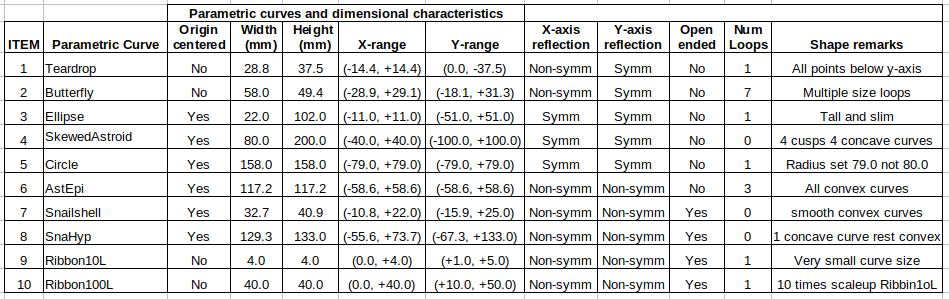
\includegraphics[width=1.70\textwidth]{Images/Chap3/Parametric-Curve-shapes-and-dimensions.png} 
	\end{figure}	
\end{landscape}

%% ===============================================
\clearpage
\pagebreak

\section{Links to parametric curves}

\noindent
The following links will jump directly to the figures and their parametric equations.

\begin{enumerate}
	\item Teardrop curve Fig [\ref{Teardrop-curve-plot-BW.pdf}]
	
	\item Teardrop comparison: Zhong et. al.(2018) Fig [\ref{Comparison-Teardrop-Zhong-et-al-2018.png}]
	
	\item Butterfly curve Fig [\ref{Butterfly-curve-plot-BW.pdf}]
	
	\item Butterfly NURBS comparison: Ni et. al.(2018) Fig [\ref{Comparison-Butterfly-Ni-et-al(2018)}]
	
	\item Butterfly NURBS comparison: Hu et. al.(2023) Fig [\ref{Comparison-Butterfly-Hu-et-al(2023)}]
	
	\item Ellipse curve Fig [\ref{Ellipse-curve-plot-BW.pdf}]
	
	\item SkewedAstroid curve Fig [\ref{SkewedAstroid-curve-plot-BW.pdf}]
	
	\item Circle Fig [\ref{Circle-curve-plot-BW.pdf}]
	
	\item AstEpi curve Fig [\ref{AstEpi-curve-plot-BW.pdf}]
	
	\item Snailshell curve Fig [\ref{Snailshell-curve-plot-BW.pdf}]
	
	\item SnaHyp curve Fig [\ref{SnaHyp-curve-plot-BW.pdf}]
	
	\item Ribbon10L curve Fig [\ref{Ribbon10L-curve-plot-BW.pdf}]
	
	\item Ribbon100L curve Fig [\ref{Ribbon100L-curve-plot-BW.pdf}]
	
	\item Ribbon B-Splines comparison: Zhong-et-al(2018) Fig [\ref{Comparison-Ribbon-Zhong-et-al(2018)}]
	
	
\end{enumerate}



%% ===============================================
\clearpage
\pagebreak

\begin{figure}
	\caption{Teardrop shape profile}
	\label{Teardrop-curve-plot-BW.pdf}
	\centering
	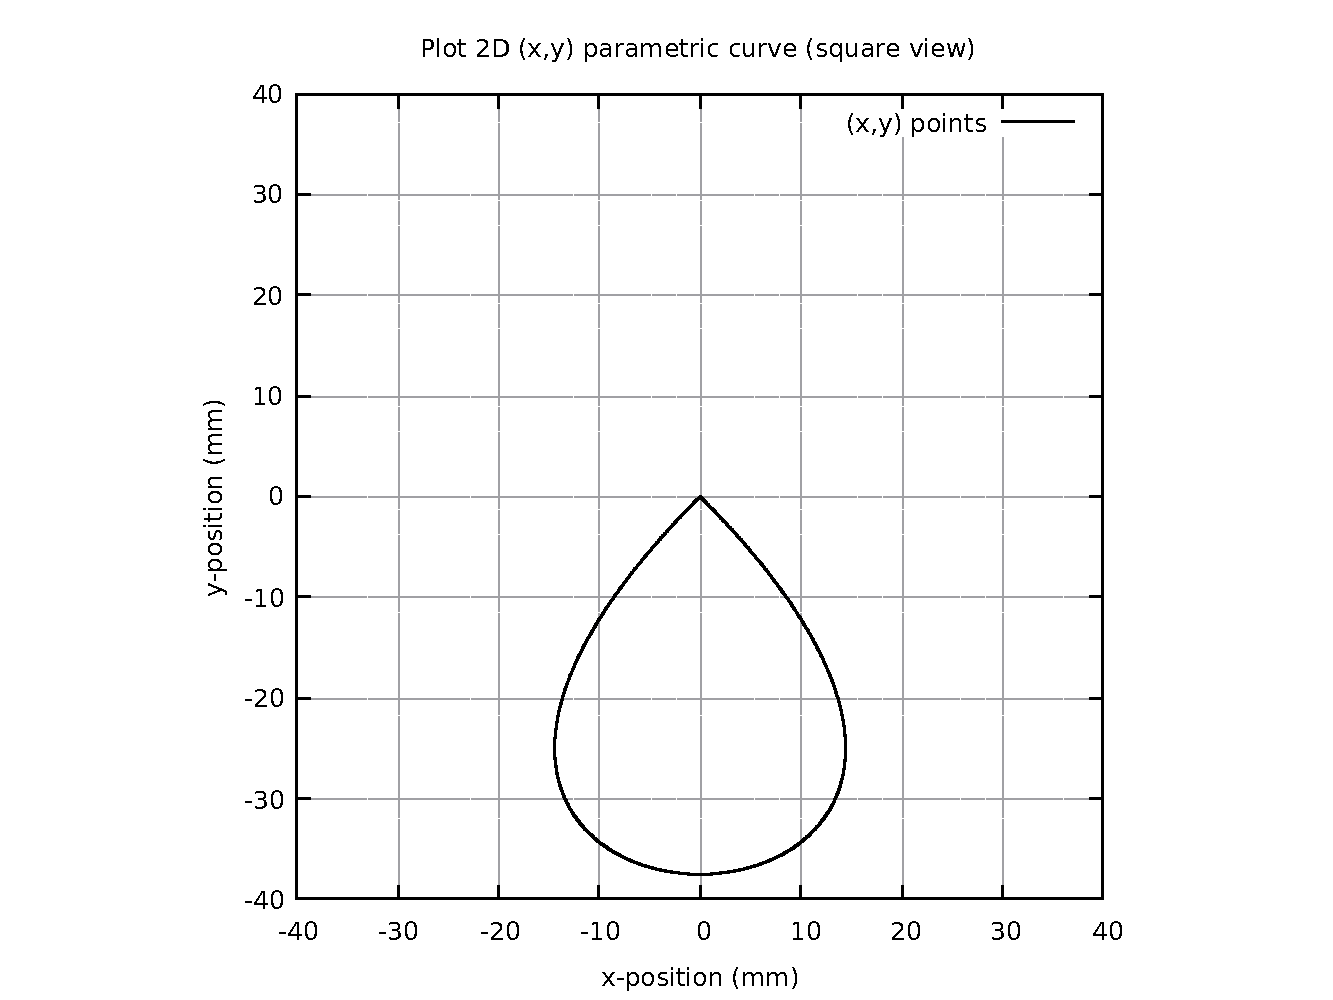
\includegraphics[width=1.00\textwidth]{Chap3/curve-shape/curves/Teardrop-curve-plot-BW.pdf} 
\end{figure}

\begin{table}[ht]
	\begin{center}
		\begin{tabular}{ p{16.0cm} }
			\caption{Teardrop curve parametric equation}
			\begin{eqnarray}
				x(u) & = & - 150u + 450u^2 - 300u^3 \nonumber \\   
				y(u) & = & - 150u + 150u^2 \nonumber \\
				u & \in & [0.0, 1.0] \nonumber
			\end{eqnarray}
		\end{tabular}
	\end{center}
\end{table}

%% TEARDROP ZHONG COMPARISONS
%% ====================
\clearpage
\pagebreak

\begin{figure}
	\caption{Teardrop comparison Zhong et. al. (2018) }
	\label{Comparison-Teardrop-Zhong-et-al-2018.png}
	\centering
	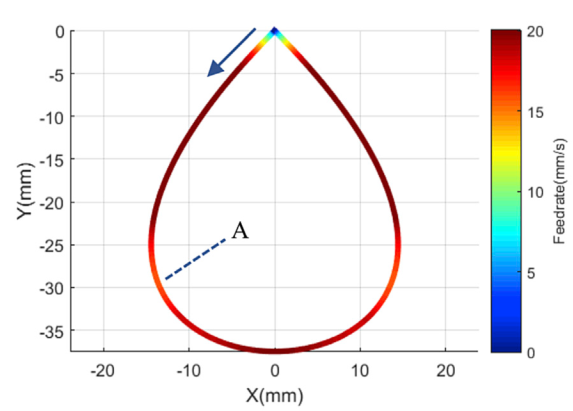
\includegraphics[width=0.750\textwidth]{Images/Chap3/Comparison-Teardrop-Zhong-et-al-2018.png} 
\end{figure}

This figure by Zhong et. al. (2018) above is identical to the one used in this work because the same parametric equation was used. Even though the interpolation method is different, the results are similar but not identical. The flowchart in their work is complex and complicated to understand. As a comparison, the flowchart and algorithm in this work is simpler, and computations are fully functionalized and modularized.\\

Notice that this Teardrop figure by Zhong et. al. (2018) above is plotted on a rectangular grid (x and y intervals are not the same size), instead of a square grid done in this work shown in Fig [\ref{Teardrop-curve-plot-BW.pdf}]. This rectangular grid gives a false impression of a wider bottom for the Teardrop, that actually is not the case.\\ 

In addition, the Teardrop figure by Zhong is not presented in an overall grid that is square and origin-centered. It does not provide information on the placement of the Teardrop location relative to the origin. This origin-centered presentation provides information regarding the x and y axes reflection symmetry for the particular curve. \\



%% BUTTERFLY CURVE EQUATION
%% ====================
\clearpage
\pagebreak

\begin{figure}
	\caption{Butterfly shape profile}
	\label{Butterfly-curve-plot-BW.pdf}
	\centering
	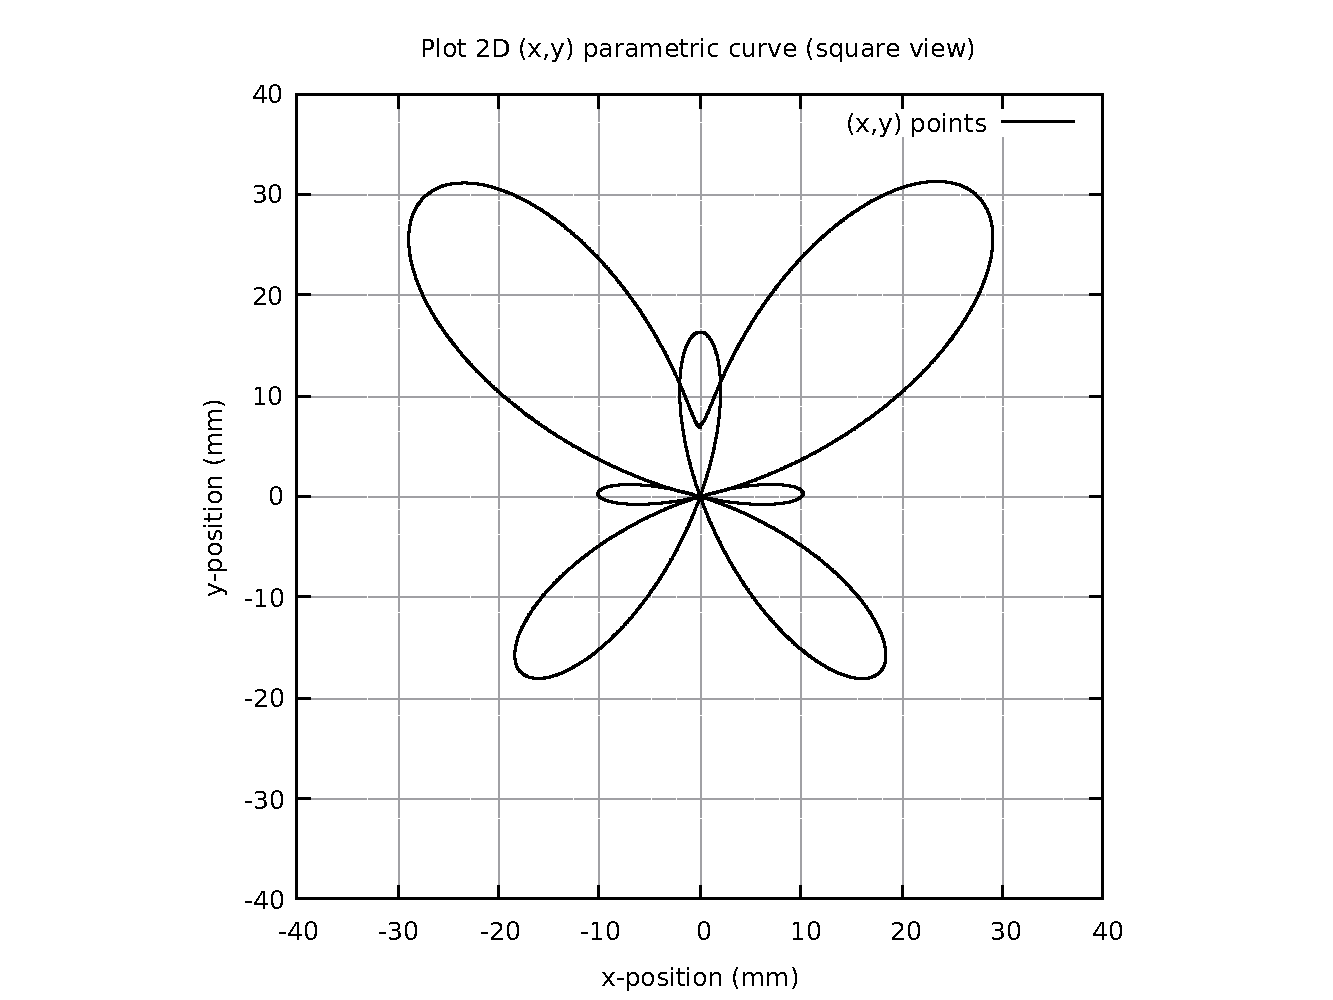
\includegraphics[width=1.00\textwidth]{Chap3/curve-shape/curves/Butterfly-curve-plot-BW.pdf} 
\end{figure}

\begin{table}[ht]
\begin{center}
\begin{tabular}{ p{16.0cm} }
\caption{Butterfly curve parametric equation}
\begin{eqnarray}
	x(u) & = & \sin(2\pi u) \left [ e^{\cos(2\pi u)} - 2\cos(8\pi u) - (\sin(2\pi u/12))^5 \right] \nonumber \\
	y(u) & = & \cos(2\pi u) \left [ e^{\cos(2\pi u)} - 2\cos(8\pi u) - (\sin(2\pi u/12))^5 \right] \nonumber \\
	u & \in & [0.0, 1.0] \nonumber
\end{eqnarray}
\end{tabular}
\end{center}
\end{table}


%% ==========================================
\clearpage
\pagebreak

%% BUTTERFLY COMPARISON 1
\begin{figure}
	\caption{Butterfly comparison Ni et. al. (2018) NURBS}
	\label{Comparison-Butterfly-Ni-et-al(2018)}
	\centering
	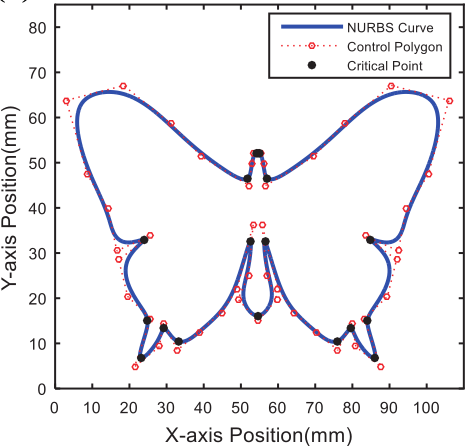
\includegraphics[width=0.70\textwidth]{Images/Chap3/Comparison-Butterfly-Ni-et-al-2018.png} 
\end{figure}

%% BUTTERFLY COMPARISON 2
\begin{figure}
	\caption{Butterfly comparison Hu et. al. (2023) NURBS }
	\label{Comparison-Butterfly-Hu-et-al(2023)}
	\centering
	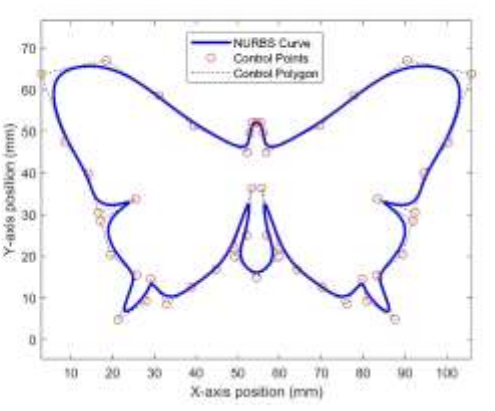
\includegraphics[width=0.78\textwidth]{Images/Chap3/Comparison-Butterfly-Hu-et-al-2023.png} 
\end{figure}

%% \noindent Note: The original is not clear.
%% ============================================

%% ELLIPSE CURVE EQUATION
%% ====================
\clearpage
\pagebreak

\begin{figure}
	\caption{Ellipse shape profile}
	\label{Ellipse-curve-plot-BW.pdf}
	\centering
	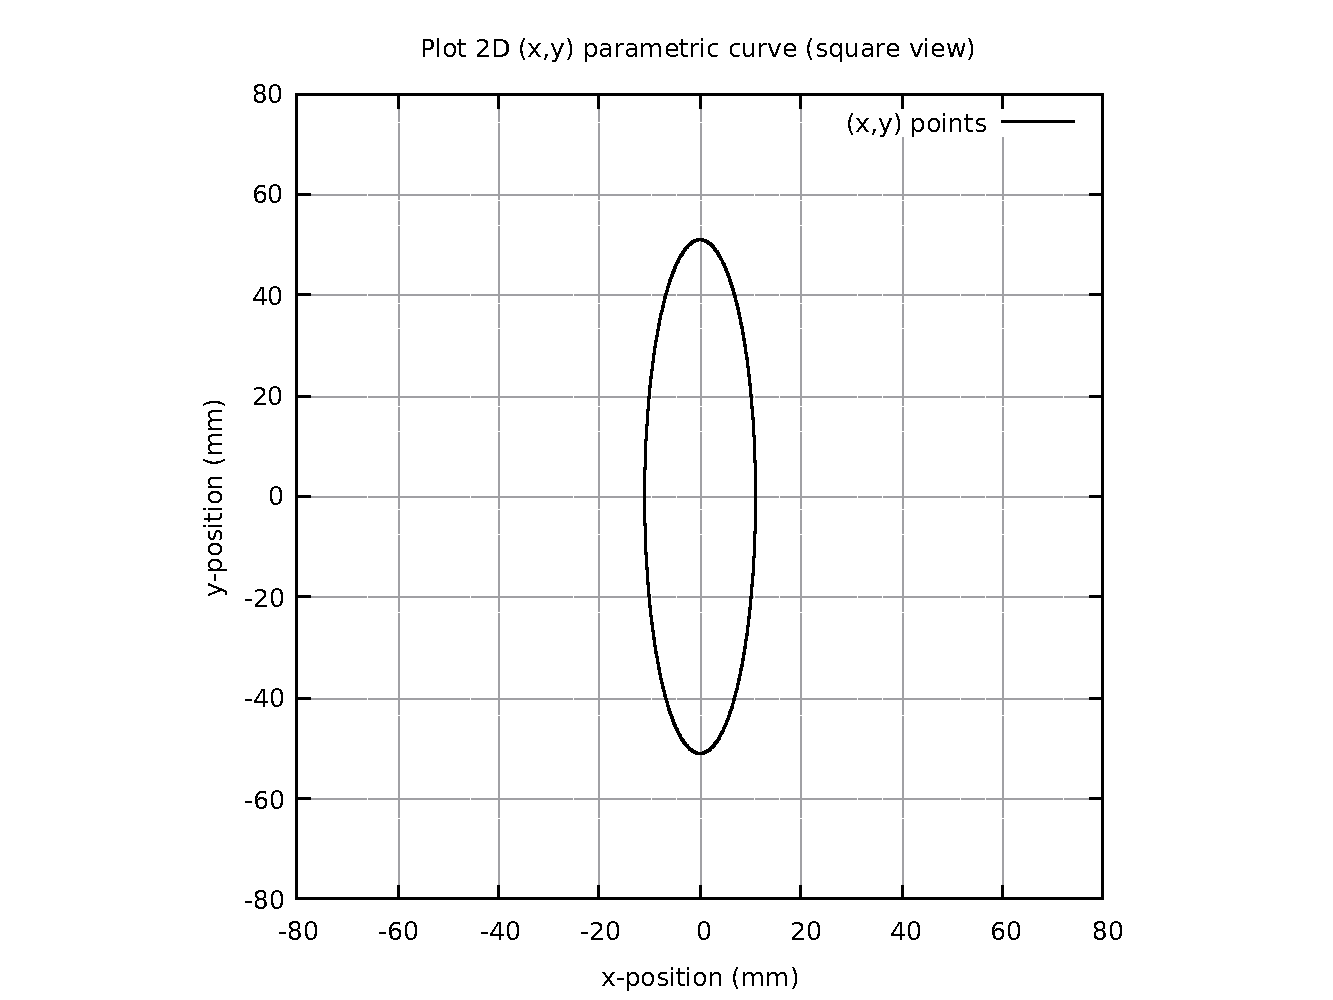
\includegraphics[width=1.20\textwidth]{Chap3/curve-shape/curves/Ellipse-curve-plot-BW.pdf} 
\end{figure}

\begin{table}[ht]
\begin{center}
\begin{tabular}{ p{16.0cm} }
\caption{Ellipse curve parametric equation}
\begin{eqnarray}
	x(u) & = & 11\sin(2\pi u) \nonumber \\   
	y(u) & = & 51\cos(2\pi u) \nonumber \\
	& \in & [0.0, 1.0] \nonumber
\end{eqnarray}
\end{tabular}
\end{center}
\end{table}


%% SKEWEDASTROID CURVE EQUATION
%% ====================
\clearpage
\pagebreak

\begin{figure}
	\caption{SkewedAstroid shape profile}
	\label{SkewedAstroid-curve-plot-BW.pdf}
	\centering
	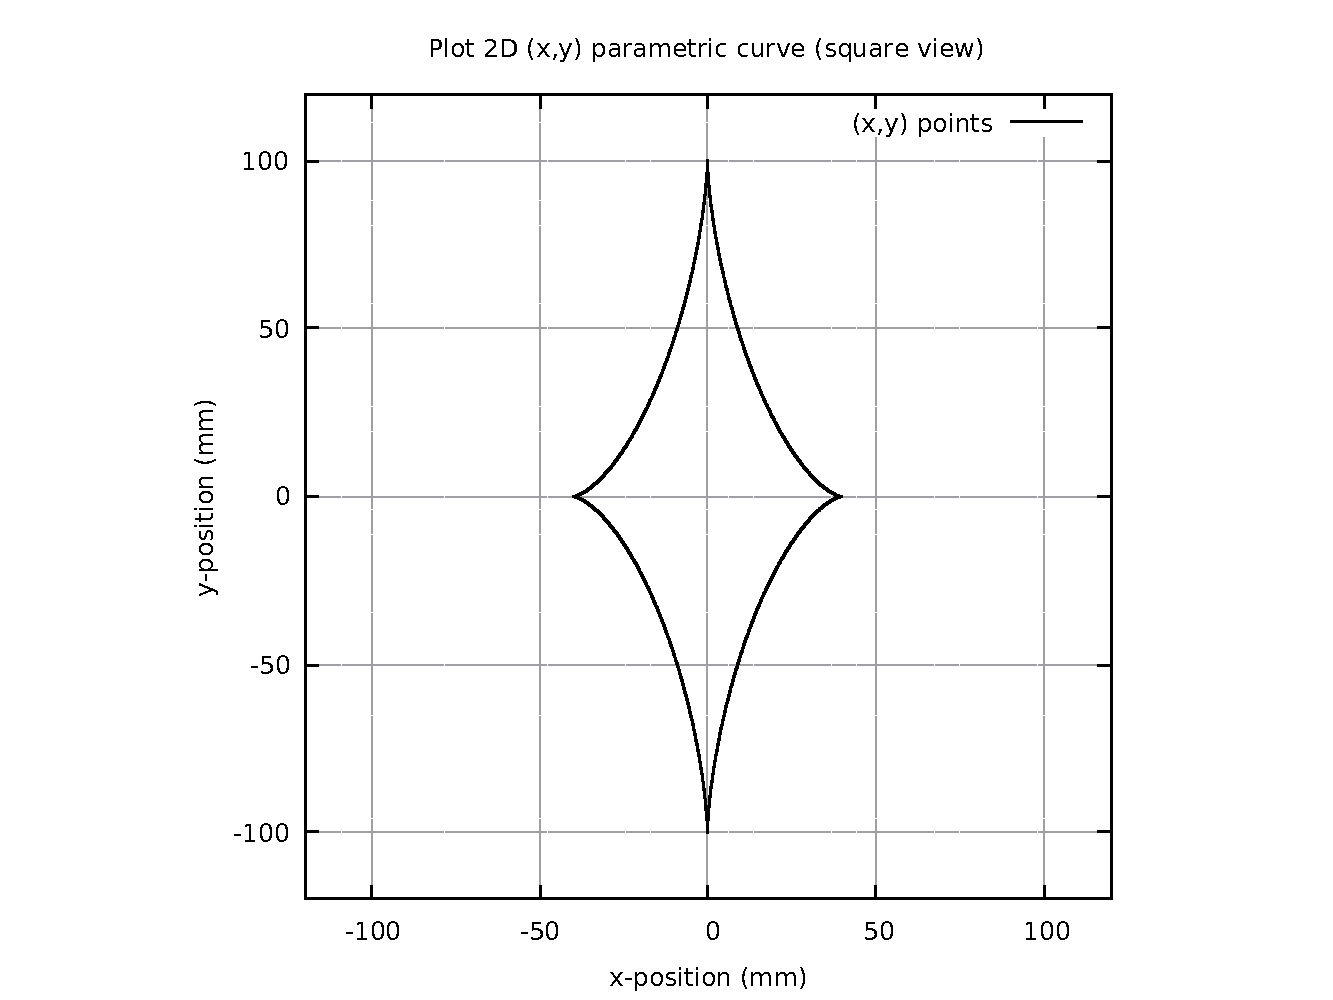
\includegraphics[width=1.20\textwidth]{Chap3/curve-shape/curves/SkewedAstroid-curve-plot-BW.pdf} 
\end{figure}

\begin{table}[ht]
\begin{center}
\begin{tabular}{ p{16.0cm} }
\caption{SkewedAstroid curve parametric equation}
\begin{eqnarray}
	x(u) & = & 40  [ \sin(2\pi u) ]^3  \nonumber \\
	y(u) & = & 100 [ \cos(2\pi u) ]^3  \nonumber \\
	u & \in & [0.0, 1.0] \nonumber
\end{eqnarray}
\end{tabular}
\end{center}
\end{table}

%% CIRCLE
%% ==================================================
\clearpage
\pagebreak

\begin{figure}
	\caption{Circle shape profile}
	\label{Circle-curve-plot-BW.pdf}
	\centering
	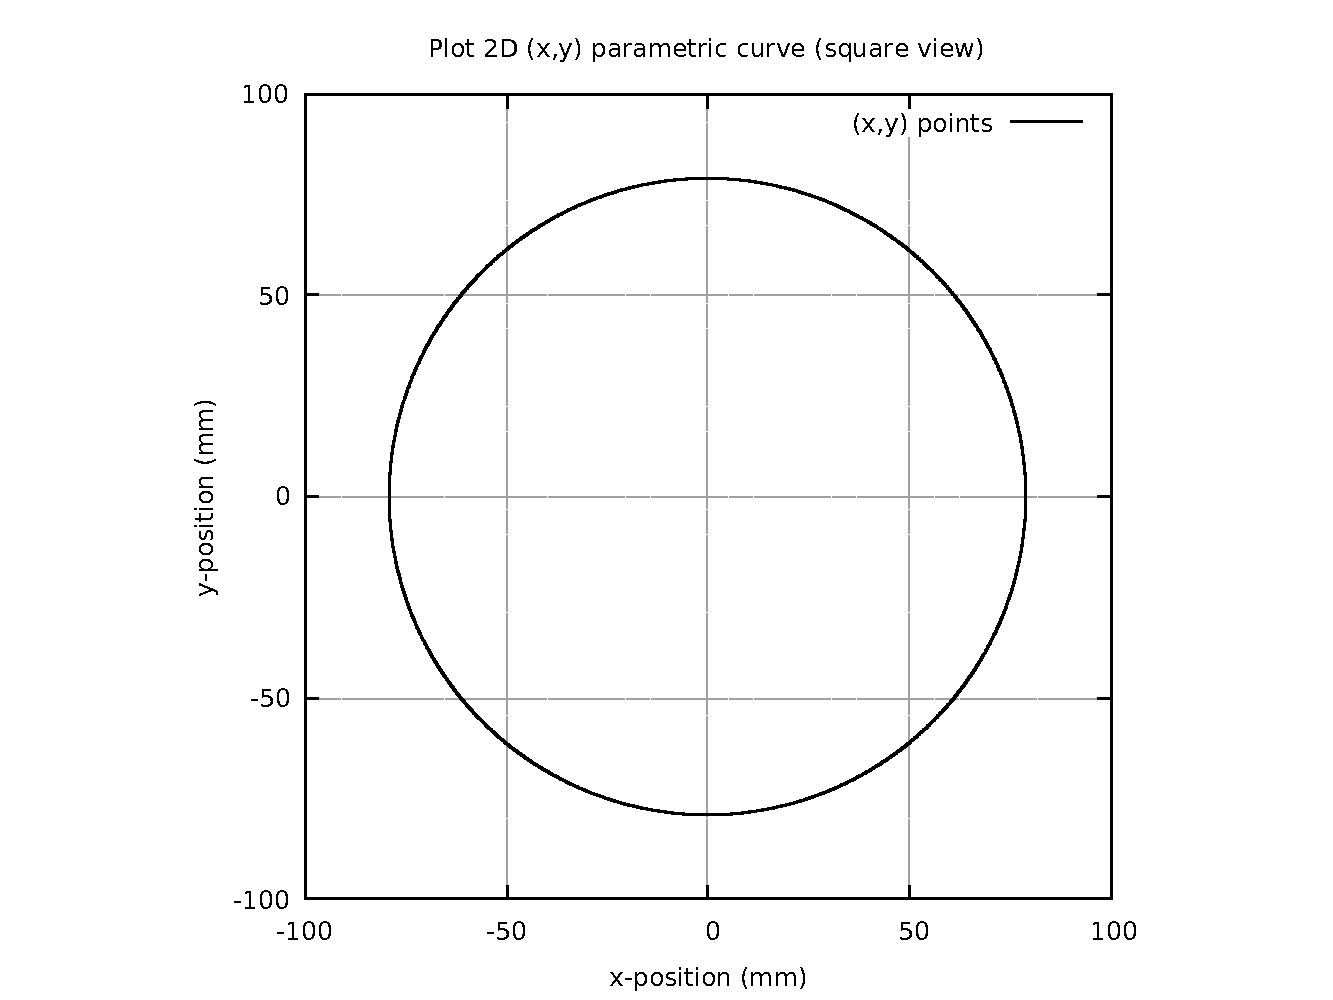
\includegraphics[width=1.20\textwidth]{Chap3/curve-shape/curves/Circle-curve-plot-BW.pdf} 
\end{figure}

\begin{table}[ht]
\begin{center}
\begin{tabular}{ p{16.0cm} }
\caption{Circle parametric equation}
\begin{eqnarray}
	x(u) & = & 79\sin(2\pi u) \nonumber \\   
	y(u) & = & 79\cos(2\pi u) \nonumber \\
	u & \in & [0.0, 1.0] \nonumber
\end{eqnarray}
\end{tabular}
\end{center}
\end{table}

%% ASTEPI 
%% ==================================================
\clearpage
\pagebreak

\begin{figure}
	\caption{AstEpi shape profile}
	\label{AstEpi-curve-plot-BW.pdf}
	\centering
	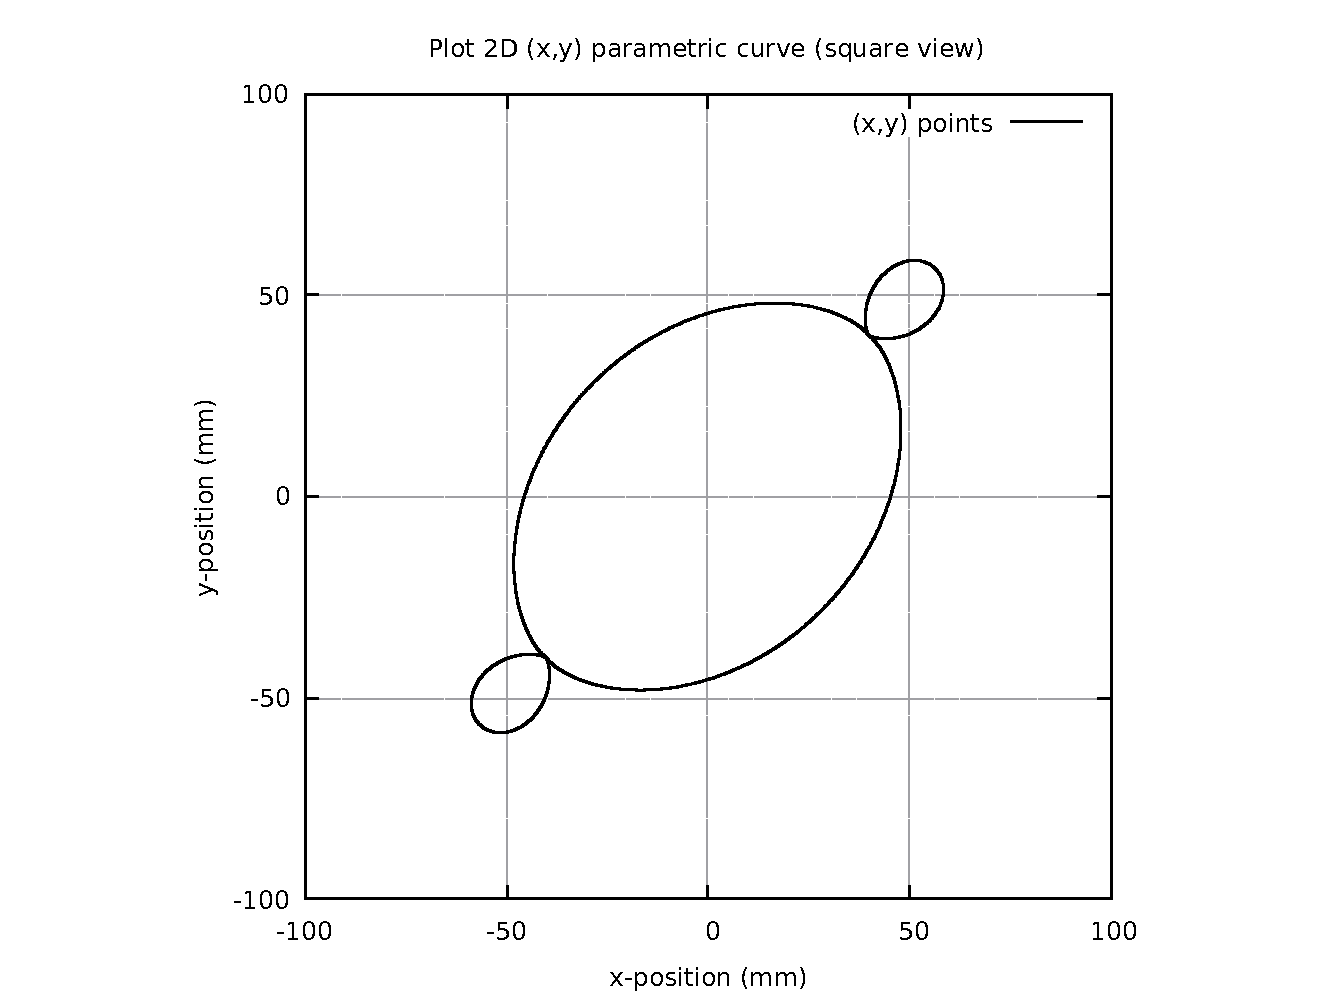
\includegraphics[width=1.20\textwidth]{Chap3/curve-shape/curves/AstEpi-curve-plot-BW.pdf} 
\end{figure}


\begin{table}[ht]
\begin{center}
\begin{tabular}{ p{16.0cm} }
\caption{AstEpi curve parametric equation}
\begin{eqnarray}
	tvtiny & = & 0.0000000001 \nonumber \\
	x(u) & = & 40[\sin(2\pi u)]^3 + 50\cos(2\pi u + tvtiny) - 10\cos(10\pi u -tvtiny) \nonumber \\
	y(u) & = & 40[\cos(2\pi u)]^3 + 50\sin(2\pi u + tvtiny) - 10\sin(10\pi u -tvtiny) \nonumber \\
	u & \in & [0.0, 1.0] \nonumber
\end{eqnarray}
\end{tabular}
\end{center}
\end{table}

%% SNAILSHELL
%% ==================================================
\clearpage
\pagebreak

\begin{figure}
	\caption{Snailshell shape profile}
	\label{Snailshell-curve-plot-BW.pdf}
	\centering
	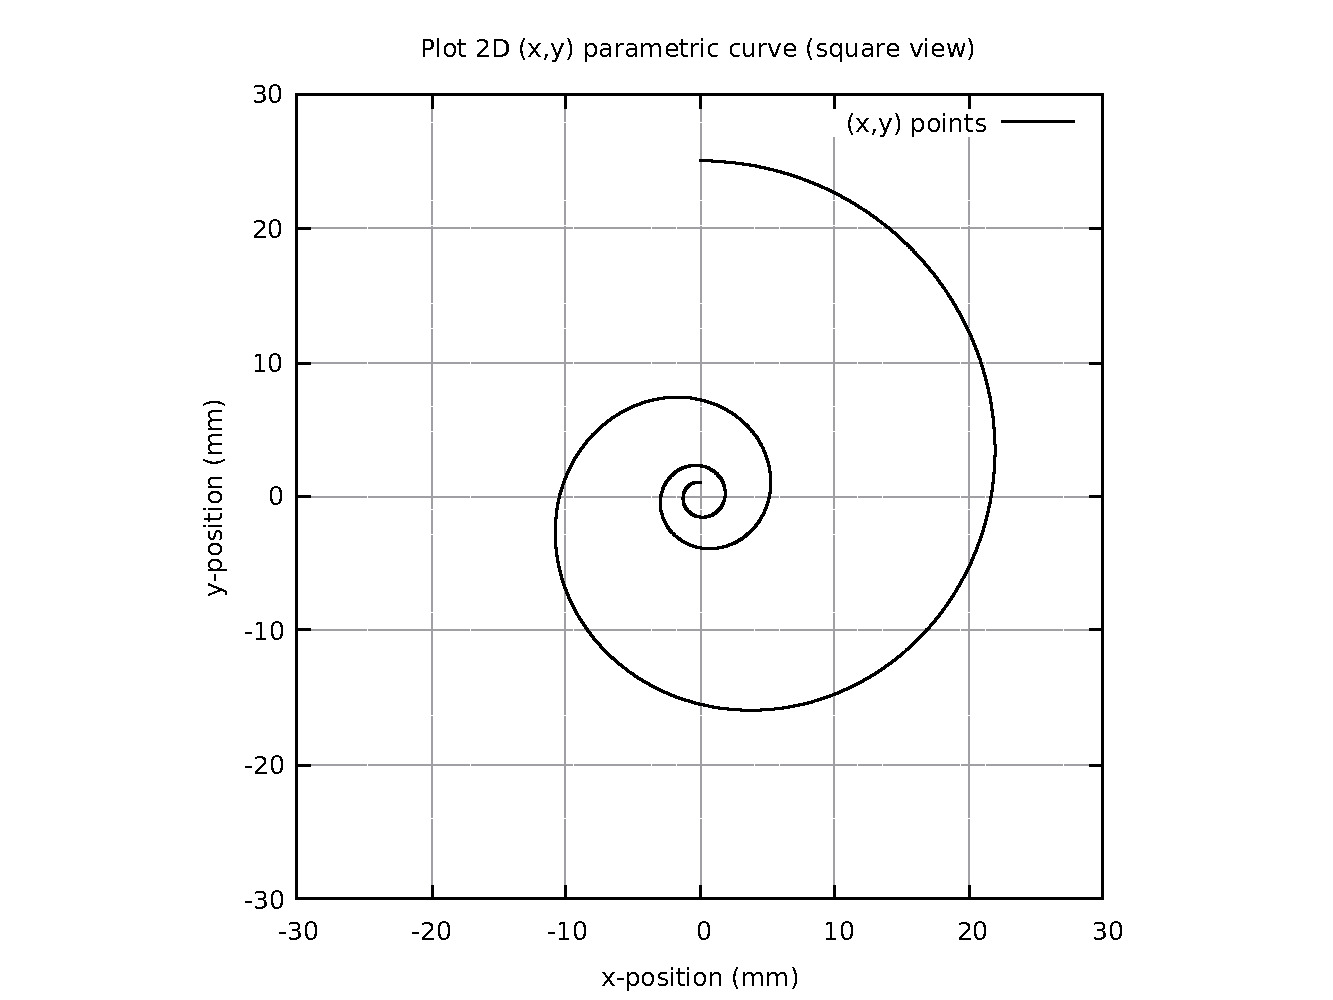
\includegraphics[width=1.20\textwidth]{Chap3/curve-shape/curves/Snailshell-curve-plot-BW.pdf} 
\end{figure}


\begin{table}[ht]
\begin{center}
\begin{tabular}{ p{16.0cm} }
\caption{Snailshell curve parametric equation}
\begin{eqnarray}
	x(u) & = & 100\sin(6\pi u) / [9 (\pi u)^2 + 4] \nonumber \\   
	y(u) & = & 100\cos(6\pi u) / [9 (\pi u)^2 + 4] \nonumber \\
	u & \in & [0.0, 1.0] \nonumber
\end{eqnarray}
\end{tabular}
\end{center}
\end{table}


%% SNAHYP
%% ==================================================
\clearpage
\pagebreak

\begin{figure}
	\caption{SnaHyp shape profile}
	\label{SnaHyp-curve-plot-BW.pdf}
	\centering
	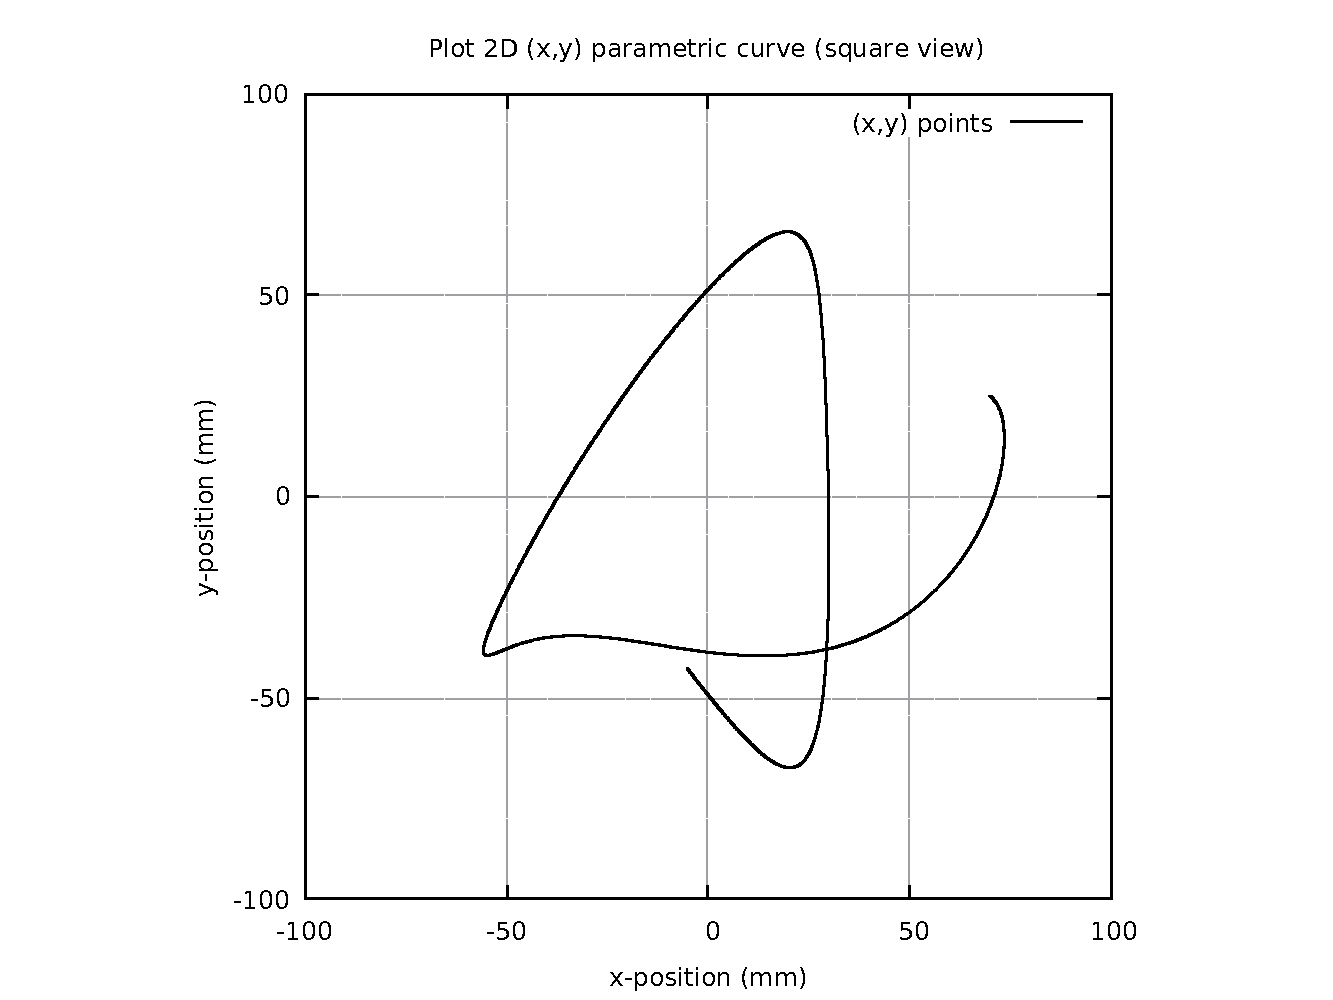
\includegraphics[width=1.20\textwidth]{Chap3/curve-shape/curves/SnaHyp-curve-plot-BW.pdf} 
\end{figure}

\begin{table}[ht]
\begin{center}
\begin{tabular}{ p{16.0cm} }
\caption{SnaHyp curve parametric equation}
\begin{eqnarray}
	xsna(u) & = & [4\sin(8\pi u) ] / [16 (\pi u)^2 + 4] \nonumber \\
	xhyp(u) & = & [2\cos(4\pi u)  + 5\cos(8\pi u /3)  ] \nonumber \\
	x(u) & = & 10[xsna(u) + xhyp(u)] \nonumber \\
	ysna(u) & = & [10\cos(8\pi u)] / [16 (\pi u)^2 + 4] \nonumber \\
	yhyp(u) & = & [2\sin(8\pi u) - 5\sin(8\pi u /3)] \nonumber \\
	y(u) & = & 10[ysna(u) + yhyp(u)] \nonumber \\
	u & \in & [0.0, 1.0] \nonumber
\end{eqnarray}
\end{tabular}
\end{center}
\end{table}

%% RIBBON10L
%% ==================================================
\clearpage
\pagebreak

\begin{figure}
	\caption{Ribbon10L shape profile}
	\label{Ribbon10L-curve-plot-BW.pdf}
	\centering
	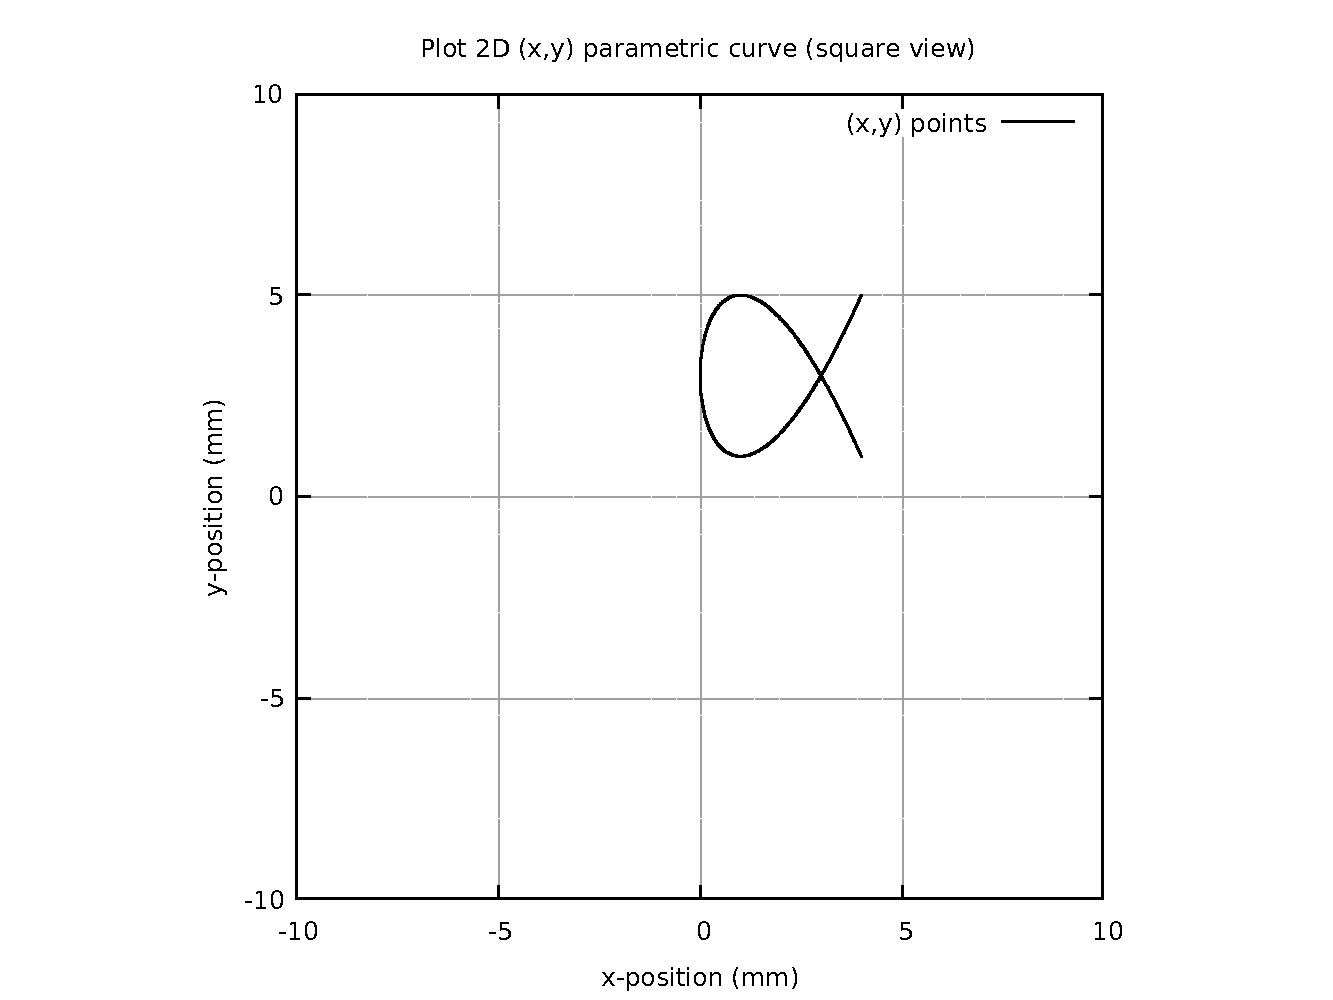
\includegraphics[width=1.20\textwidth]{Chap3/curve-shape/curves/Ribbon10L-curve-plot-BW.pdf} 
\end{figure}

\begin{table}[ht]
\begin{center}
\begin{tabular}{ p{16.0cm} }
\caption{Ribbon10L curve parametric equation}
\begin{eqnarray}
	t(u) & = & 4(u - 0.50) \nonumber \\
	x(u) & = & t^2 \nonumber \\   
	y(u) & = & t^3 - 3t + 3 \nonumber \\
	u & \in & [0.0, 1.0] \nonumber
\end{eqnarray}
\end{tabular}
\end{center}
\end{table}

%% Ribbon100L
%% ==================================================
\clearpage
\pagebreak

\begin{figure}
	\caption{Ribbon100L shape profile}
	\label{Ribbon100L-curve-plot-BW.pdf}
	\centering
	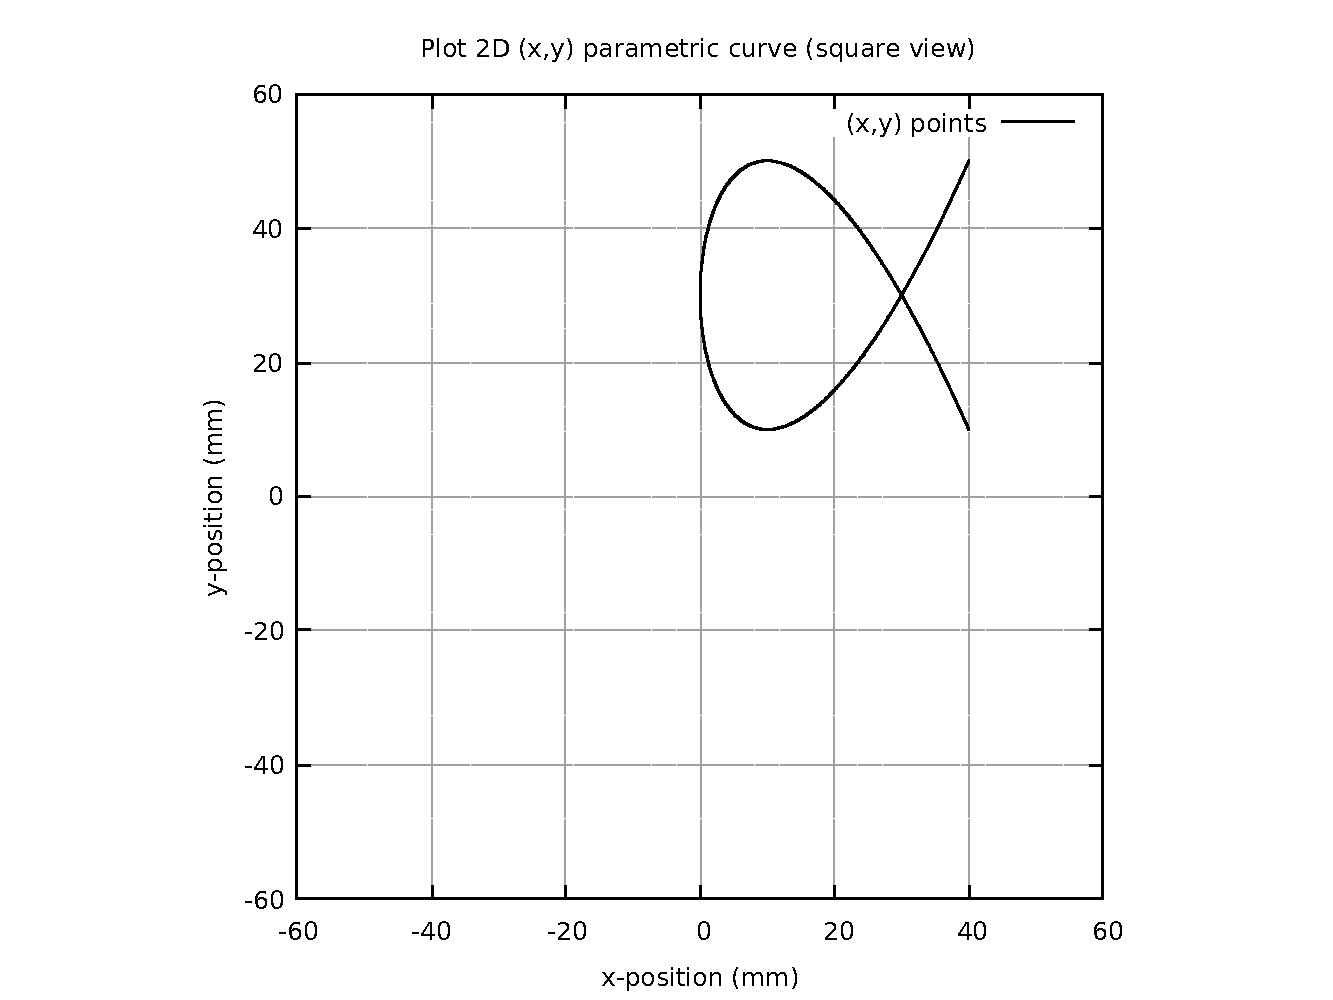
\includegraphics[width=1.20\textwidth]{Chap3/curve-shape/curves/Ribbon100L-curve-plot-BW.pdf} 
\end{figure}

\begin{table}[ht]
\begin{center}
\begin{tabular}{ p{16.0cm} }
\caption{Ribbon100L curve parametric equation}
\begin{eqnarray}
	t(u) & = & 4(u - 0.50) \nonumber \\
	x(u) & = & 10t^2 \nonumber \\   
	y(u) & = & 10t^3 - 30t + 30 \nonumber \\
	u & \in & [0.0, 1.0] \nonumber
\end{eqnarray}
\end{tabular}
\end{center}
\end{table}


%% RIBBON ZHONG COMPARISONS
%% ====================
\clearpage
\pagebreak

\begin{figure}
	\caption{Ribbon comparison Zhong et. al. (2018) B-Splines}
	\label{Comparison-Ribbon-Zhong-et-al(2018)}
	\centering 
	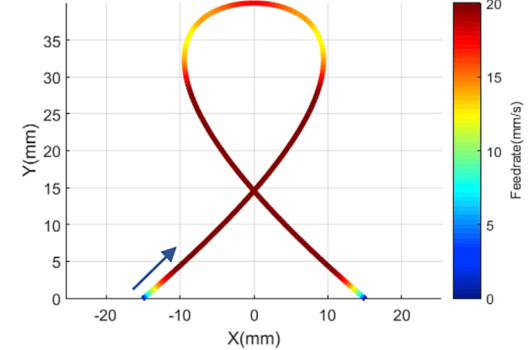
\includegraphics[width=0.80\textwidth]{Images/Chap3/Comparison-Ribbon-Zhong-et-al-2018.png} 
\end{figure}

Compared to this work which uses the standard third degree polynomial for the Ribbon curve, the representation by \cite{Zhong-etal:2018} is a NURBS type, 3rd degree B-Spline with control points\\

$\{P_{i}\} = \{ (-15,0), (20,30), (0,50), (-20,30), (15,0)  \}$ \\
and knot vectors $U = \{0, 0, 0, 0, 0.5, 1, 1, 1, 1\}$.\\

NURBS or Non-Uniform Rational B-Splines are a generalization of B-Splines. Note that NURBS can create smooth and precise shapes that can be scaled, rotated, and deformed without losing quality. Splines are simpler curves that are defined by a set of control points and a degree of smoothness.\\



%% ==================================
\clearpage
\pagebreak

\section{Direction of travel in parametric curves}

With a 3D plot of the Teardrop curve, direction of traversal of the $u$ point can be easily visualized. It begins from $u=0$ to $u=1$. Upon collapsing the $u(t)$ axis, it becomes a 2D Teardrop closed curve again. This means parametric interpolations provide direction of traversal for curves and surfaces through the parameter $u(t)$. \\

\begin{figure}
	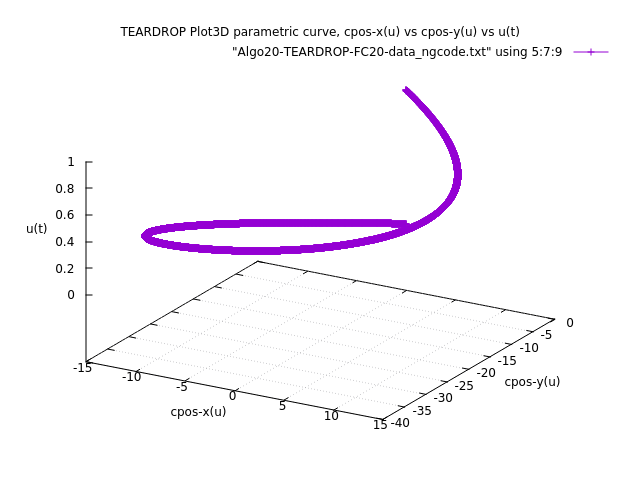
\includegraphics[width=1.10\textwidth]{Chap4/images/TEARDROP-plot-3D-x-vs-y-vs-u.png} 
	\label{TEARDROP-plot3D-data_ngcode.png}
	\caption{Teardrop 3D plot x(u) vs y(u) vs u(t)}
\end{figure}

\clearpage
\pagebreak

\begin{figure}
	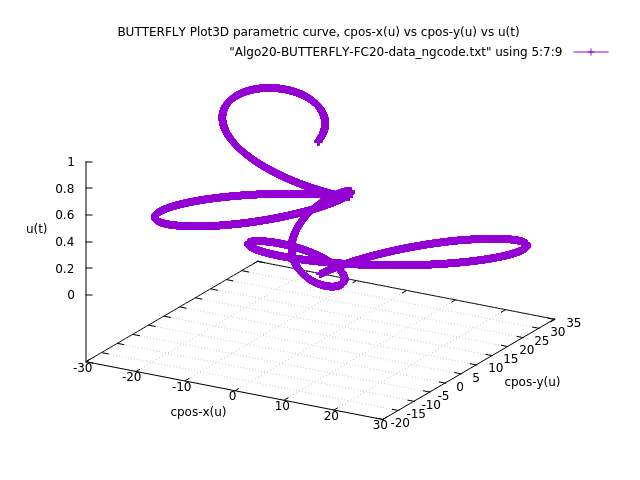
\includegraphics[width=1.10\textwidth]{Chap4/images/BUTTERFLY-plot-3D-x-vs-y-vs-u.png} 
	\label{BUTTERFLY-plot3D-data_ngcode.png}
	\caption{Butterfly 3D plot x(u) vs y(u) vs u(t)}
\end{figure}


The 3D plot for the Butterfly looks messy but the principle is the same. When the $u(t)$ axis collapses, it becomes a 2D Butterfly closed curve again.


%% ==================================================
%% ==================================================
\clearpage
\pagebreak

\section{Chord-error concept}

\begin{figure}
	\caption{Chord-error eps ($\epsilon$), Feedrate F, and Interpolation time T}
	\label{Chord-error-image.png}
	\centering
	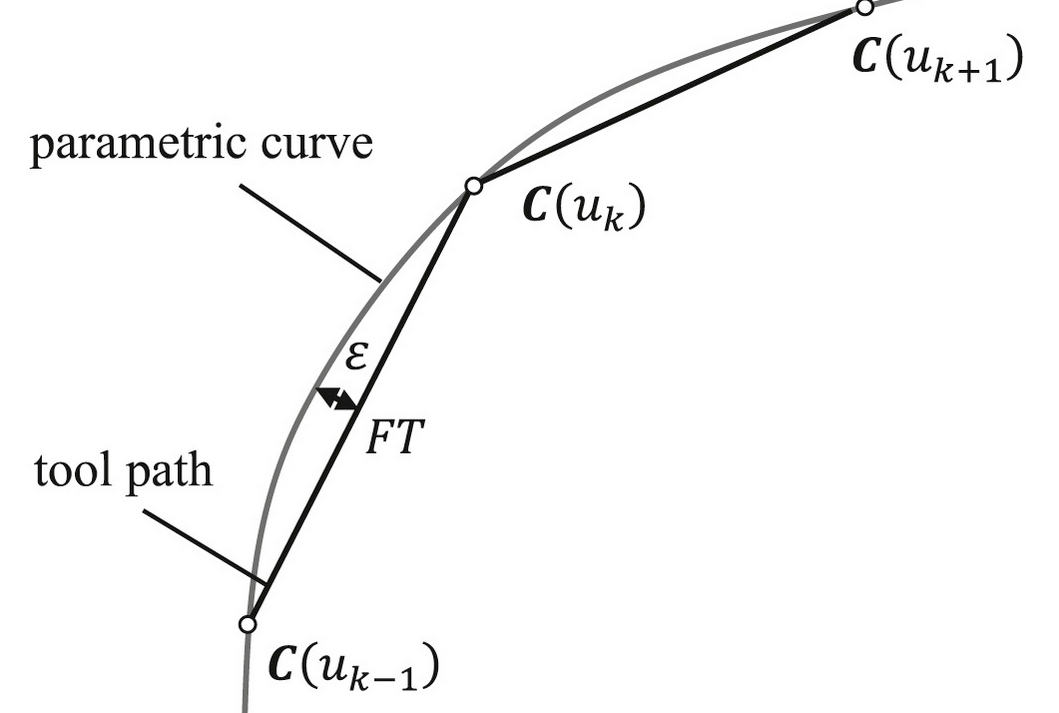
\includegraphics[width=0.80\textwidth]{Images/Chap3/Chord-error-image.png} 


\end{figure}

The relationship between the parametric curve, chord-error and machine feedrate is illustrated in the Fig [\ref{Chord-error-image.png}] above. (Source: \cite{Zhong-etal:2018}) It shows 3 successive interpolated points $C(u_{k-1})$, $C(u_{k})$ and $C(u_{k+1})$ as the parameter is incremented from $u_{k-1}$ to  $u_{k}$ and  $u_{k+1}$ along the parametric curve. \\

The chord is defined as the line connecting two points on the parametric curve. The chord-error $\epsilon$ is the maximum distance of a line from the curve perpendicular to the chord. If F is the feedrate (mm/s) and T is the interpolation period (s), that is, time duration to move from one point to the next, then the product of feedrate with interpolation time gives the length of the chord (FT).\\

The calculation method for the chord-error ($\epsilon$) between two points on the parametric curve is described in section Chord-error $eps(u)$ [\ref{chap3-Chord-error eps}].

\section{Chord-error minimization}

A decrease in the chord length (FT), will cause a decrease the chord-error ($\epsilon$). This is favorable for accuracy since the toolpath follows closer to the path trajectory of the parametric curve. However, decreasing the chord-length causes an increase in the number of interpolated points for the same length of the curve. Since the interpolation time for a single step is a constant, this will also increase the total machining time, a feature that is not favorable. 
 
\section{Feedrate maximization}

An increase in feedrate (F) of the CNC machining tool, will decrease the total machining time. This is favourable for faster completion of machining for the same length of the curve. However, the increase in feedrate will cause a larger chord length (FT), thus a larger chord-error ($\epsilon$).

\section{Chord-error and feedrate constraints}

The approach in this work is to establish a combined chord-error and feedrate constraint. It is based on the following:

\begin{enumerate}
	\item A strict maximum chord-error value is set as the error-tolerance. Every move in the interpolated point-to-point traversal must not exceed this error-tolerance. 
	
	\item Every move in the interpolated point-to-point traversal must not exceed the calculated feedrate limit for that particular point.

    \item The feedrate limit at any particular point is calculated based on a combined geometric, dynamic and kinematic factors of the particular CNC machine. 
	
\end{enumerate}

\section{Brief on algorithm strategy and design}

In This-Work, the realtime parametric curve algorithm will be designed to iterate every point-to-point, as step move, such that the chord-error is below error-tolerance and the current feedrate is close but below the feedrate limit, that is, before the next move is taken. This is the criteria of iterative convergence. The cycle repeats until the point-to-point traversal of the entire parametric curve is completed.\\

Without exception, the flowcharts in This-Work are all of the type, "one way in and one way out". This strategy or paradigm is called "structured programming". Every functional computation unit implemented in this realtime interpolation algorithm comply with this structured programming strategy. In addition, various reports were generated, written to text files,  to capture every variable change and transaction during the execution of the algorithm. This facilitates very easy search, analysis and debugging. \\

About structured programming algorithms, the following two(2) figures in the next section are basic examples of structured programming algorithms. Fig[\ref{img-Example-1-Structured Programming Design}] and Fig[\ref{img-Example-2-Structured Programming Design}] show the basic sequence and iterative loop. Both examples exhibit features of program flows in a "one way in and one way out" pattern. \\

About non-structured programming algorithms, the next two(2) figures demonstrate its features. The program flow in this case is difficult to track and so not easy to comprehend. Fig[\ref{img-Example-3-Non-Structured Programming Design}] shows overlapping flows in functional units "B" and "X" nodes, while Fig[\ref{img-Example-4-Non-Structured Programming Design}], is considered non-structured programming because there is "one-way-in but four-ways-out". \\	

%% ==================================================
\clearpage
\pagebreak

\begin{figure}
	\centering
	\caption  {Example-1-Structured Programming Design (1-in, 1-out)}
	\label{img-Example-1-Structured Programming Design}
	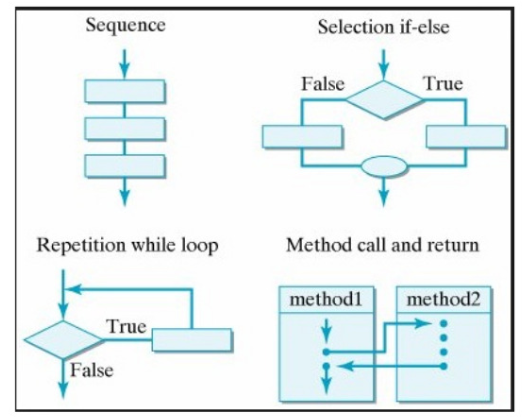
\includegraphics[width= 0.80\textwidth]{Chap3/AlgorithmTypes/Example-1-Structured-Programming-design.png} 
\end{figure}		


\begin{figure}
	\centering
	\caption  {Example-2-Structured Programming Design (1-in, 1-out)}
	\label{img-Example-2-Structured Programming Design}
	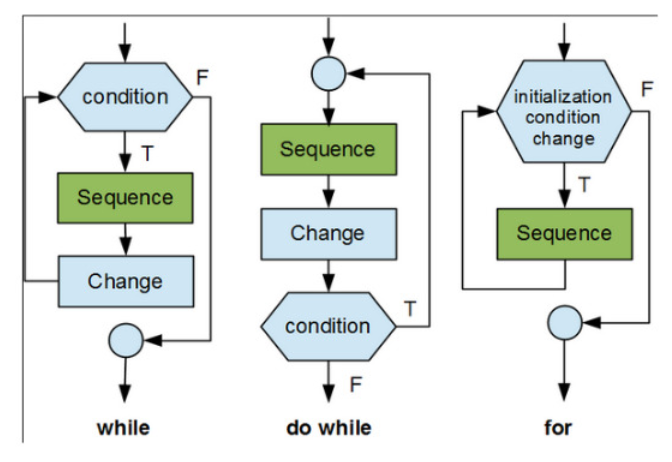
\includegraphics[width= 0.80\textwidth]{Chap3/AlgorithmTypes/Example-2-Structured-Programming-design.png} 
\end{figure}		

%% =======================================================
\clearpage
\pagebreak

\begin{figure}
	\centering
	\caption  {Example-3-Non-Structured Programming Design, (S=Start, E=Exit)}
	\label{img-Example-3-Non-Structured Programming Design}
	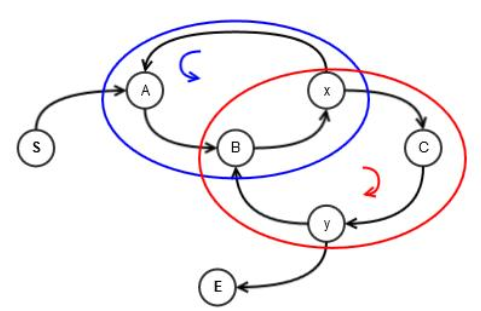
\includegraphics[width= 0.70\textwidth]{Chap3/AlgorithmTypes/Example-3-Non-Structured-Programming-design.png} 
\end{figure}		



\begin{figure}
	\centering
	\caption  {Example-4-Non-Structured Programming Design (1-in, 4-outs)}
	\label{img-Example-4-Non-Structured Programming Design}
	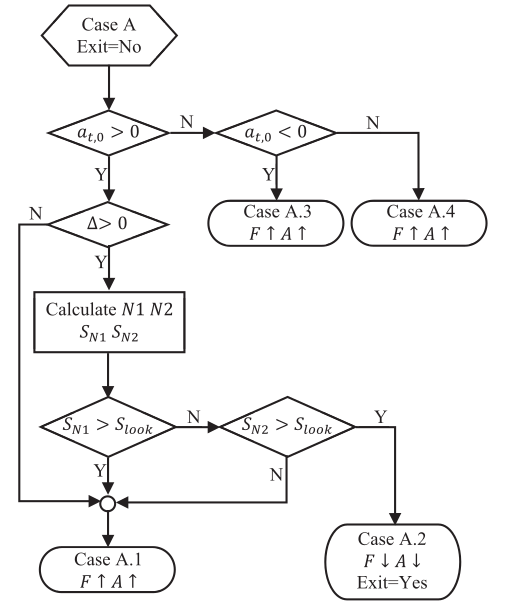
\includegraphics[width= 0.60\textwidth]{Chap3/AlgorithmTypes/Example-4-Non-Structured-Programming-design.png} 
\end{figure}		



%% ==================================================
\clearpage
\pagebreak

\section{Radius of Curvature $\textbf{rho(u)}$}

The radius of curvature ($R$ or $rho$) is important in inspection of curves and surfaces. The value of $rho$ is the reciprocal of curvature, $K$. So $rho = (1/K)$. For a curve, $rho(u)$ equals the radius of circular arc which best approximates the curve at that point $u$. The curvature $K$, is the amount by which a curve deviates from being a straight line, or a surface deviates from being a plane (not flat).\\

Note that the radius of curvature $rho(u)$ is constant for a circle over all applicable values of parameter $u$. Essentially, the value of $rho(u)$ is just the radius of the circle itself. \\ 

Consider a series of concentric circles with the radii increasing from zero to some large number. Intuitively, an increasing $rho(u)$ value means the curvature opens to a larger and larger circle radius. On the contrary, a decreasing $rho(u)$ value means the curvature closes to a smaller and smaller circle radius. 


%% \clearpage
%% \pagebreak


When $rho(u)$ becomes zero, the curve shrinks to a single point and there is no curvature or curving behaviour. When $rho(u)$ value reaches infinity, it becomes a straight line and there is also no curving behaviour. This is an important general rule when visually inspecting curves and surfaces.\\

If the curve is given parametrically by functions $x(u)$ and $y(u)$, then from standard calculus and analytic geometry, the exact derivation for radius of curvature is given by:

\[ R(u) = rho(u) = \Bigg | \frac{numerator(u)}{denominator(u)} \Bigg |  \]
\[ K(u) = curvature(u) =  \Bigg | \frac{denominator(u)}{numerator(u)} \Bigg |  \]
where 
\[ numerator(u) = \Bigg ( \Bigg ({\odv{x(u)}{u}} \Bigg )^{2} + \Bigg ({\odv{y(u)}{u}}\Bigg )^{2} \Bigg ) ^{3/2}  \]
\[ denominator(u) = \Bigg(\odv{x(u)}{u}\Bigg)\Bigg(\frac{\mathrm{d^2}y(u)}{\mathrm{d}u^2}\Bigg) - \Bigg(\frac{\mathrm{d^2}x(u)}{\mathrm{d}u^2}\Bigg)\Bigg(\odv{y(u)}{u}\Bigg)  \]


%% $
%% \frac{\mathrm{d^2}y(u)}{\mathrm{d}u^2} 
%%
%% \frac{\mathrm{d^2}x(u)}{\mathrm{d}u^2}
%% $ 


% ================================
%% \clearpage
%% \pagebreak

\section{Chord-error $\textbf{eps(u)}$}
\label{chap3-Chord-error eps}

The chord-error (epsilon) is the maximum length of the line perpendicular to the chord from a point on the arc segment. Based on extensive computer simulations, it was found that the perpendicular line starting from the mid-point on the chord that intersects the arc segment gives the maximum length. The algorithm for calculating $eps(u)$ is as follows:

\begin{enumerate}
	\item From the current u-point giving an $C(x(u), y(u))$ point on the parametric curve, determine the $C(x(u+next), y(u+next))$ point value on the curve. This is just the next interpolated point on the curve. 
	
	\item Construct a chord line between the points $C(x(u), y(u))$ and $C(x(u+next), y(u+next))$. Calculate the slope of this chord line. Call it $chordslope$.
	
	\item From geometry, any line that is perpendicular to this chord will have a slope of $perplineslope = (-1/chordslope)$.
	
	\item Find the mid-point coordinates $x_{mid}$ and $y_{mid}$ on this chord line.
	
	\item From the known $chordslope$ and chord mid-point coordinates, generate a linear equation perpendicular to this line. Call it the $perpline$.
	
	\item Find the intersection coordinates of the given parametric curve (arc segment) with the $perpline$. Call these coordinates $x_{int}$ and $y_{int}$. 
	
	\item The calculated value of chord-error $eps(u)$ is the linear length between the points ($x_{mid}$,$y_{mid}$) and ($x_{int}$ and $y_{int}$).
	
	\item The linear length is calculated using the standard Pythagoras formula in Cartesian coordinates.
	
\end{enumerate}

% ================================
%% \clearpage
%% \pagebreak
\begin{figure}
	\centering
	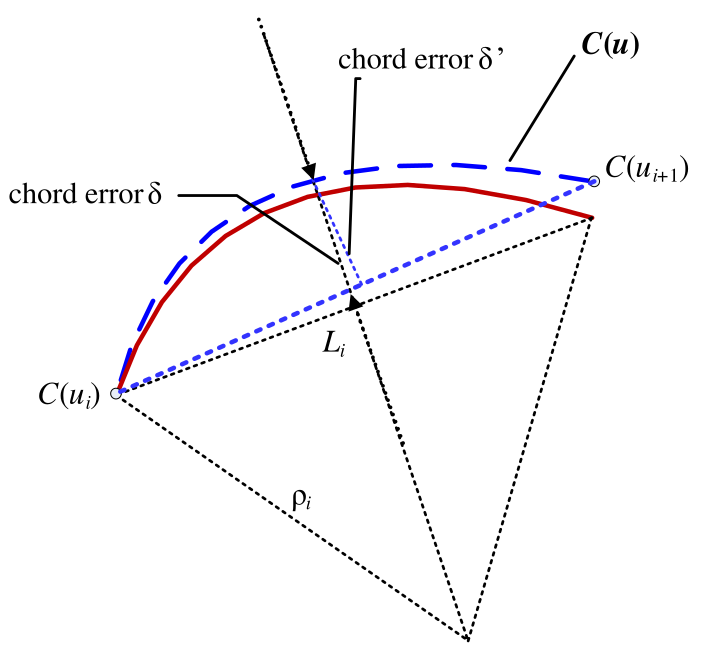
\includegraphics[width=0.60\textwidth]{Images/Chap3/Chord-error-between-2-interpolated-points.png} 
	\caption{Chord-error between two interpolated points}
	\label{Chord-error-between-2-interpolated-points.png}
\end{figure}

\clearpage
\pagebreak


\section{Feedrate or Velocity $ \textbf{V(u)} $}

This section describes the derivation of feedrate or velocity ($V(u_{i})$) from the radius of curvature ($rho(u_{i})$) and chord-error ($eps(u_{i})$). For a linear distance traveled (chord distance) between $C(u_{i})$ and $C(u_{i+1})$, denoted by $L_{i}$, the velocity is given by

\[ V(u_{i}) = \frac {L_{i}} {T_{i}}  \] 

where $T_{i} = (t_{i+1} - t_{i})$  is the interpolation time. Since an arc approximates a section of the circle, the chord error $eps(u_{i})$, is derived from geometry as a function of the radius of curvature $rho(u_{i})$, approximately as follows:

\[ eps(u_{i}) = (radius\_to\_arc) - (radius\_to\_center\_of\_chord) \]

\[ eps(u_{i}) = rho(u_{i}) - \sqrt{{rho(u_{i})}^{2} - {(L_{i}/2)}^{2}}  \]

\vspace{0.5cm}
Solving for $L_{i}$ and replacing for $L_{i}$, the velocity is 

\[ V(u_{i}) = \frac {L_{i}} {T_{i}}   = \frac{2}{T_{i}}.\sqrt{{rho(u_{i})}^{2} - {(rho(u_{i}) - eps(u_{i}))}^{2} } \]   

% \vspace{0.5cm}


% ======================================
\clearpage
\pagebreak

\section{First order Taylor's approximation u\_next(u)}

Consider the parametric curve function C(u), and the time function u(t) as the curve parameter moves from $u(t_{i}) = u_{i}$ to $u(t_{i+1}) = u_{i+1}$. By using a Taylor's expansion, the approximation up to the first derivative is

\[ u(t_{i+1}) = u(t_{i}) + (t_{i+1} - t_{i} ).{\Bigg ( \odv{u}{t} \Bigg ) \Bigg |_{t=t_{i}}} + Higher\_order\_terms \]


\[ u_{i+1} = u_{i} + (t_{i+1} - t_{i} ).{\Bigg ( \odv{u}{t} \Bigg ) \Bigg |_{t=t_{i}}} + Higher\_order\_terms \]

The speed $V(u_{i})$ with respect to time at $u_{i}$ from the parametric curve $C(u)$ is 

\[  V(u_{i}) = \Bigg ( \odv{C(u)}{u} \Bigg ) \Bigg |_{u=u_{i}}. \Bigg ( \odv{u}{t} \Bigg ) \Bigg |_{t=t_{i}} \]

Rearranging the equation 

\[ {\Bigg ( \odv{u}{t} \Bigg ) \Bigg |_{t=t_{i}}} = \frac {V(u_{i})} {\Bigg ( \odv{C(u)}{u} \Bigg ) \Bigg |_{u=u_{i}}} \]

The Taylor's expansion now becomes

\[ u_{i+1} = u_{i} + (t_{i+1} - t_{i} ). \frac {V(u_{i})} {\Bigg ( \odv{C(u)}{u} \Bigg ) \Bigg |_{u=u_{i}}} + Higher\_order\_terms \]
\vspace{0.5cm} 

Neglecting the higher order terms and with the interpolation time or step time defined as $T_{i} = (t_{i+1} - t_{i})$  
\[ u_{i+1} = u_{i} +   unext1(u)\]
\[ u_{i+1} = u_{i} +  \frac {(T_{i}).V(u_{i})} {\Bigg ( \odv{C(u)}{u} \Bigg ) \Bigg |_{u=u_{i}} }\]
\vspace{0.5cm} 

Note that the denominator cannot be zero.

% ================================
\clearpage
\pagebreak

\section{Second order Taylor's approximation u\_next(u)}

\noindent Define the interpolation time $T_{i} = (t_{i+1} - t_{i})$    
\vspace{0.5cm}   

%% $
%% \frac{\mathrm{d^2}u(t)}{\mathrm{d}t^2} 
%%
%% \frac{\mathrm{d^2}x(u)}{\mathrm{d}u^2}
%% $ 


By using a Taylor's expansion, the approximation up to the second derivative is

\[ u(t_{i+1}) = u(t_{i}) + (T_{i}).{\Bigg ( \frac{\mathrm{d}u(t)}{\mathrm{d}t}  \Bigg ) \Bigg |_{t=t_{i}}} + \frac{T_{i}^{2}}{2}.{\Bigg ( \frac{\mathrm{d^2}u(t)}{\mathrm{d}t^2} \Bigg ) \Bigg |_{t=t_{i}}} + Higher\_order\_terms \]

Neglecting the higher order terms,

\[ u(t_{i+1}) = u(t_{i}) + (T_{i}).{\Bigg ( \frac{\mathrm{d}u(t)}{\mathrm{d}t} \Bigg ) \Bigg |_{t=t_{i}}} + \frac{T_{i}^{2}}{2}.{\Bigg ( \frac{\mathrm{d^2}u(t)}{\mathrm{d}t^2}  \Bigg ) \Bigg |_{t=t_{i}}} \]

\[\Bigg (  \frac{\mathrm{d^2}u(t)}{\mathrm{d}t^2} \Bigg ) =  \odv{\Bigg (\frac{\mathrm{d}u(t)}{\mathrm{d}t}   \Bigg)}{t} = \odv{f(t)}{t}  \]

\vspace{0.5cm}  

Given arbitrary functions f(t), g(t) and h(t), where: 
\[ f(t) = \frac {g(t)}{h(t)} \]

The Quotient Rule says that the derivative of a quotient is the denominator times the derivative of the numerator minus the numerator times the derivative of the denominator, all divided by the square of the denominator. Using the quotient rule for the derivative gives:

\[ \odv{f(t)}{t} = \frac { h(t). \Bigg( \odv{g(t)}{t} \Bigg) - g(t).\Bigg( \odv{h(t)}{t} \Bigg)} {( h(t) )^{2}  } \]

With the function f(t) calculated previously

\[ f(t) = \Bigg ( \odv{u(t)}{t} \Bigg )  =  \frac {V(u_{i})} {\Bigg ( \odv{C(u)}{u} \Bigg ) \Bigg |_{u=u_{i}}} \]

\[ \odv{f(t)}{t}  = \Bigg ( \frac{\mathrm{d^2}u(t)}{\mathrm{d}t^2}  \Bigg ) = \odv{\Bigg( g(t)/h(t) \Bigg) }{t}  \]
where
\[ g(t) = V(u_{i}) \]
\[ h(t) = \Bigg ( \odv{C(u)}{u} \Bigg ) \Bigg |_{u=u_{i}}\]

Substitute g(t) and h(t) into the quotient rule equation and rearranging

\[ \odv{f(t)}{t} = \Bigg ( \frac{\mathrm{d^2}u(t)}{\mathrm{d}t^2} \Bigg )  = - {(V(u_{i}))}^{2}. \frac{A}{B} \]

\[ \Bigg ( \frac{\mathrm{d^2}u(t)}{\mathrm{d}t^2} \Bigg )  = - {(V(u_{i}))}^{2}. \frac{ \Bigg | {\Bigg (\frac{\mathrm{d^2}C(u)}{\mathrm{d}u^2} \Bigg ) \Bigg |_{u=u_{i}} } }{ \Bigg | {\Bigg ( \odv{C(u)}{u} \Bigg ) \Bigg |_{u=u_{i}} ^{3} }    }  \]

where 

\[ A = \Bigg | {\Bigg ( \frac{\mathrm{d^2}C(u)}{\mathrm{d}u^2} \Bigg ) \Bigg |_{u=u_{i}} }  \]
\[ B = \Bigg | {\Bigg ( \odv{C(u)}{u} \Bigg ) \Bigg |_{u=u_{i}} ^{3} }  \]

The second order Taylor's expansion for the function u(t) becomes
\[ u(t_{i+1}) = u(t_{i}) + (T_{i}).{\Bigg ( \odv{u}{t} \Bigg ) \Bigg |_{t=t_{i}}} + \frac{T_{i}^{2}}{2}.{\Bigg ( \frac{\mathrm{d^2}u}{\mathrm{d}t^2} \Bigg ) \Bigg |_{t=t_{i}}} \]

\[ u(t_{i+1}) = u(t_{i}) + \frac{(T_{i}.V(u_{i}))} {\Bigg ( \odv{C(u)}{u} \Bigg ) \Bigg |_{u=u_{i}}} - \frac{ (T_{i}.V(u_{i})) ^{2}}{2}. \frac{ \Bigg | {\Bigg ( \frac{\mathrm{d^2}C(u)}{\mathrm{d}u^2} \Bigg ) \Bigg |_{u=u_{i}} } }{ \Bigg | {\Bigg ( \odv{C(u)}{u} \Bigg ) \Bigg |_{u=u_{i}} ^{3} } } \]

In software implementation,
\[ u\_next = u(t_{i+1}) - u(t_{i}) \]
\[ u\_next =  \frac{(T_{i}.V(u_{i}))} {\Bigg ( \odv{C(u)}{u} \Bigg ) \Bigg |_{u=u_{i}}} - \frac{ (T_{i}.V(u_{i})) ^{2}}{2}. \frac{ \Bigg | {\Bigg (  \frac{\mathrm{d^2}C(u)}{\mathrm{d}u^2} \Bigg ) \Bigg |_{u=u_{i}} } }{ \Bigg | {\Bigg ( \odv{C(u)}{u} \Bigg ) \Bigg |_{u=u_{i}} ^{3} } } \]
where
\[ \Bigg | \Bigg ( \odv{C(u)}{u} \Bigg ) \Bigg |_{u=u_{i}}  = fxn\_cvel\_magn(u) \]
\[ \Bigg | \Bigg ( \frac{\mathrm{d^2}C(u)}{\mathrm{d}u^2} \Bigg ) \Bigg |_{u=u_{i}} = fxn\_cacc\_magn(u) \]

\[  T_{i}    = (t_{i+1} -t_{i}) = implementation\_time\_selected     \]
\[  V(u_{i}) = velocity\_command\_or\_feedrate\_generated\_by\_some\_function \]

% =======================================
%% \clearpage
%% \pagebreak

\section{Next interpolation point calculation}

In the realtime interpolation algorithm, the next interpolation point $u\_next$ is calculated based on Taylor's expansion as follows. Note that for $u\_next$ to be valid, the denominators cannot be zero.\\

\textbf{First order Taylor's approximation}
\[ u\_next = \frac {(T_{i}).V(u_{i})} {\Bigg ( \odv{C(u)}{u} \Bigg ) \Bigg |_{u=u_{i}} } \]
\vspace{0.5cm}

\textbf{Second order Taylor's approximation}
\[ u\_next =  \frac{(T_{i}.V(u_{i}))} {\Bigg ( \odv{C(u)}{u} \Bigg ) \Bigg |_{u=u_{i}}} - \frac{ (T_{i}.V(u_{i})) ^{2}}{2}. \frac{ \Bigg | {\Bigg ( \frac{\mathrm{d^2}C(u)}{\mathrm{d}u^2} \Bigg ) \Bigg |_{u=u_{i}} } }{ \Bigg | {\Bigg ( \odv{C(u)}{u} \Bigg ) \Bigg |_{u=u_{i}} ^{3} } } \]
\vspace{0.5cm}

The above are the two(2) equations to be used in software implementation. Notice the negative value of the second term in the Second order Taylor's approximation. \\

It is important to note that all of the derivatives (first and second order) are executed on the curve C(u) with respect to  parameter u. The time parameter t is no longer in the equation. Essentially, the Taylor's approximation used here "transforms" the u\_next point in terms of u instead of t. The starting point is u being a "function of t, that is, u(t)".\\



% ======================================================

% ======================================================
\clearpage
\pagebreak

\section{Feedrate limit calculations}

The current feedrate limit is the minimum of four(4) separate feedrate limits denoted by $ \Big (fratelimit\_1, fratelimit\_2, fratelimit\_3, fratelimit\_4 \Big)$. The limits are based on geometrical and dynamical constraints described below. \\

\begin{table}[!ht]
\begin{center}
%% \caption{Feedrate limit parameters}	
%% \label{Feedrate-limit-parameters}	
\begin{tabular}{ p{2.0cm} p{13.0cm} }
%% \hline
    $fratelimit\_1$ & = frate\_command, a user specified feedrate constraint value\\   
& \\
	$fratelimit\_2$ & = dynamic constraint on machine maximum X-Y axial velocities \\   
& \\
	$fratelimit\_3$ & = geometric constraint on chord-error or contour accuracy \\   
& \\
	$fratelimit\_4$ & = dynamic constraint on machine maximum X-Y axial accelerations \\   
& \\
%% \hline
\end{tabular}
\end{center}
\end{table}

\noindent The functional form for the current feedrate limit becomes: \\

\noindent feedrate\_limit = $\textbf{min}\Big (fratelimit\_1, fratelimit\_2, fratelimit\_3, fratelimit\_4 \Big)$ \\

\noindent The current feedrate limit at $u$ is caclulated as a function of the following variables.\\

\begin{table}[!ht]
	\begin{center}
		\caption{Feedrate limit function parameters}	
		\label{Feedrate-limit-parameters}	
		\begin{tabular}{ p{3.0cm} p{11.0cm} }
			\hline 
			$rt$               & = current runtime in seconds \\
			$u$                & = current $u$ parameter value \\
			$u\_next$          & = next interpolated $u$ parameter value \\
			$FC$               & = user specified feedrate command (constant) value  \\
			$T$                & = interpolation step time (constant 0.001) in seconds\\
			$rho$              & = radius of curvature at current $u$ value  \\ 
			$eps$              & = chord-error (epsilon) at current $u$ value \\
			$lambda$           & = safety factor for acceleration (a constant, range 0.0 - 1.0) \\ 
			$xVel_{max}$ & = maximum allowable x-axis velocity of the machine \\
			$yVel_{max}$ & = maximum allowable y-axis velocity of the machine \\
			$xAcc_{max}$ & = maximum allowable x-axis acceleration of the machine \\
			$yAcc_{max}$ & = maximum allowable y-axis acceleration of the machine \\
			$alphaVel$   & = magnitude of x-velocity unit vector at current $u$\\
			$betaVel$    & = magnitude of y-velocity unit vector at current $u$\\
			\hline
		\end{tabular}
	\end{center}
\end{table}

It is important to note that the feedrate limit calculations for the Teardrop curve were conducted as a comparison to the work of \cite{Zhong-etal:2018}. The calculations overall were different, but the resulting feedrate profiles were similar. This work however, produces a much smoother feedrate profile. 


%% ==================================================
\clearpage
\pagebreak

\subsection{Feedrate Limit 1}

\begin{table}[ht]
\begin{center}
\begin{tabular}{ p{14.0cm} }
\caption{Calculation for fratelimit\_1}
\begin{eqnarray}
	fratelimit\_1 & = & user\_assigned\_fixed\_value (e.g. 20) \nonumber
\end{eqnarray}
\end{tabular}
\end{center}
\end{table}

The machining feedrate during correct machine operation should never exceed this user assigned feedrate value. Thus, $fratelimit\_1$ is the absolute maximum limit, and therefore, appropriately termed as the $feedrate\_command$. For a perfect and ideal operation, the machine should be running at this feedrate value throughout the curve path. This should happen for a path that is exactly a straight line.

\subsection{Feedrate Limit 2}

\begin{table}[ht]
\begin{center}
\begin{tabular}{ p{14.0cm} }
\caption{Calculation for fratelimit\_2}
\begin{eqnarray}
	alphaVel(u) & = &  \Bigg | \frac { \Bigg (\odv{x(u)}{u} \Bigg) } { \sqrt { \Bigg( {\odv{x(u)}{u}} \Bigg )^{2} +  \Bigg ( {\odv{y(u)}{u}} \Bigg )^{2} } }  \Bigg |  \nonumber \\
	betaVel(u)  & = &  \Bigg | \frac { \Bigg (\odv{y(u)}{u} \Bigg) } { \sqrt { \Bigg( {\odv{x(u)}{u}} \Bigg )^{2} +  \Bigg ( {\odv{y(u)}{u}} \Bigg )^{2} } }  \Bigg |  \nonumber \\
    A & = & xVel_{max} / alphaVel(u) \nonumber \\
    B & = & yVel_{max} / betaVel(u)  \nonumber \\   
    fratelimit\_2 & = & minimum (A, B) \nonumber 
\end{eqnarray}
\end{tabular}
\end{center}
\end{table}

The $fratelimit\_2$ is dependent on both geometrical constraints $alphaVel(u)$ and $betaVel(u)$, as well as dynamical constraints, that is, the maximum allowable axial velocities of the machine as shown above ($xVel_{max}$ and $yVel_{max}$) The quantities $alphaVel(u)$, $betaVel(u)$ are essentially the magnitudes of curve unit vectors in the x and y directions, respectively. 

\subsection{Feedrate Limit 3}

\begin{table}[ht]
\begin{center}
\begin{tabular}{ p{14.0cm} }
\caption{Calculation for fratelimit\_3}
\begin{eqnarray}
numerator(u) & = & \Bigg ( \Bigg ({\odv{x(u)}{u}} \Bigg )^{2} + \Bigg ({\odv{y(u)}{u}}\Bigg )^{2} \Bigg ) ^{3/2}  \nonumber \\
denominator(u) & = & \Bigg(\odv{x(u)}{u}\Bigg)\Bigg(\frac{\mathrm{d^2}y(u)}{\mathrm{d}u^2}\Bigg) - \Bigg(\frac{\mathrm{d^2}x(u)}{\mathrm{d}u^2}\Bigg)\Bigg(\odv{y(u)}{u}\Bigg)  \nonumber \\
rho & = & numerator(u)/denominator(u) \nonumber \\
eps & = & rho - \sqrt{{rho}^{2} - {(L/2)}^{2}} \nonumber \\
fratelimit\_3 & = & (2/T)* \Bigg | \sqrt{( 2*rho*eps - eps^{2})} \Bigg | \nonumber 
\end{eqnarray}
\end{tabular}
\end{center}
\end{table}

The $fratelimit\_3$ is primarily dependent on curve geometry, as seen above involving radius of curvature $rho(u)$ and chord-error $eps(u)$. Both are dependent on the independent parameter $u$ and the curve equations. For example, a perfect circle would give a constant radius of curvature $rho(u)$ and the chord lengths would all be the same.\\

% ======================================================
\clearpage
\pagebreak

\subsection{Feedrate Limit 4}

\begin{table}[ht]
\begin{center}
\begin{tabular}{ p{16.0cm} }
\caption{Calculation for fratelimit\_4}
\begin{eqnarray}
	lamda  & = & user\_select\_safety\_factor(0.0 to 1.0)     \nonumber \\
	C & = & \sqrt {\frac{lamda*rho*xAcc_{max}} { \Bigg |(betaVel) \Bigg |} } \nonumber \\
	D & = & \sqrt {\frac{lamda*rho*yAcc_{max}} { \Bigg |(alphaVel)\Bigg |} } \nonumber \\
    fratelimit\_4 & = & minimum (C, D) \nonumber
\end{eqnarray}
\end{tabular}
\end{center}
\end{table}

The $fratelimit\_4$ is dependent on both dynamical and geometrical constraints. The dynamical constraints are in the maximum allowable axial accelerations of the machine as covered by $xAcc_{max}$ and $yAcc_{max}$. The geometrical constraints are in $alphaVel(u)$, $betaVel(u)$ and $rho(u)$.  \\

% ======================================================
\clearpage
\pagebreak


\section{Feedrate rising S-curve}

In CNC machining operation, the feedrate does not rise abruptly from zero. A smooth feedrate rise is required to ensure machine stability. 
A sigmoid S-shaped curve was selected for the rise of the current running feedrate to the current feedrate limit. \\

\[ curr\_frate(rsu) = \frac{curr\_frate\_limit(rsu)} { \Bigg( 1 + e^{(-rsu*rshape1)} \Bigg) ^{rshape2} }  \] \\

\noindent
where the applicable variable range is \\
$rsu\_start\_rise$ $\le$ $rsu$ $\le$ $rsu\_end\_rise$\\

\noindent
The linear parameter transformation from $u$ to $rsu$ is as follows:\\
$rsu$ = $rm*u$ + $rkonst$ \\

To ensure smoothness of the rising feedrate curves, simulations were conducted to determine the best values of the parameters below. These variables are user specified.\\

\begin{table}[!ht]
	\begin{center}
	\caption{Rising S-curve parameters}	
	\label{Rising-S-curve-parameters}	
	\begin{tabular}{ p{3.0cm} p{2.0cm} p{8.0cm}}
    \hline 
	rsu\_start\_rise & = 0.00  & beginning of rising S-curve \nonumber \\
	rsu\_end\_rise   & = 0.05  & end of rising S-curve \nonumber \\
	rshape1          & = 5.00  & S-curve smoothness shaping factor \nonumber \\
	rshape2          & = 8.00  & S-curve smoothness shaping factor \nonumber \\
	rsu1             & = 0.00  & start of u linear transformation\nonumber \\
	rsu2             & = 3.00  & end of u linear transformation \nonumber \\
	rm               & = calc  & slope calculated for each parametric curve \nonumber \\
	rkonst			 & = calc  & constant calculated for each parametric curve \nonumber \\ 
	rsu              & = calc  & transformed variable in the rising S-curve \nonumber \\
    \hline
	\end{tabular}
	\end{center}
\end{table}


% ===============================================
\clearpage
\pagebreak

\section{Flowchart of main interpolation program}

The main program flowchart for the parametric curve interpolation is shown in Fig [\ref{main-10-Main-Program-Algorithm.pdf}]. The parameter update u = u + u\_next is executed for each loop. As shown in the main flowchart, there are 3 main processing modules that cover computations involving u, that is, in the rising, main and falling feedrate sections. \\

The flowchart for the feedrate rising section is shown in  Fig [\ref{01-Feedrate-Rising-Region-flowchart.pdf}], and the feedrate falling section in Fig [\ref{03-Feedrate-Falling-Region-flowchart.pdf}]. The computations for the main section are further separated into 3 cases described below. 

\begin{enumerate}
	
\item When the current\_feedrate is above feedrate\_limit, called CaseA\_(Above), the flowchart is Fig [\ref{02-CaseA1-Feedrate-Above-Limit-Main-Region-flowchart.pdf}] and is continued in Fig [\ref{02-CaseA2-Feedrate-Above-Limit-Main-Region-flowchart.pdf}].

\item When the current\_feedrate is below feedrate\_limit, called CaseB\_(Below), the flowchart is Fig [\ref{02-CaseB1-Feedrate-Below-Limit-Main-Region-flowchart.pdf}] and is continued in Fig [\ref{02-CaseB2-Feedrate-Below-Limit-Main-Region-flowchart.pdf}].
 
\item When the current\_feedrate is equal to the feedrate\_limit, called CaseE (Equal), the flowchart is Fig [\ref{02-CaseE-Feedrate-Equal-Limit-Main-Region-flowchart.pdf}].

\end{enumerate}

The processing in CaseA\_(Above) is basically to push down the running current\_feedrate to just below the calculated feedrate\_limit. On the other hand, the processing in CaseB\_(Below) is to push up the current\_feedrate to also be just below the calculated feedrate\_limit. The net result is the current\_feedrate will be very close but just below the calculated feedrate\_limit.
This is the feedrate constraint part of this work. \\

A common module named Flowchart\_Calculate\_ u\_next(u), is shown in Fig [\ref{04-Calculate-u-next-flowchart.pdf}]. This module will be invoked by the feedrate rising, main and falling modules. This is the implementation of Call-and-Return (CAR) software architecture. \\

%% \clearpage
%% \pagebreak

The Flowchart\_Calculate\_u\_next(u) module will invoke another module named Flowchart\_Calculate\_u\_next(u)\_with\_eps\_pushdown, as shown in Fig [\ref{05-Calculate-u-next-eps-pushdown-flowchart.pdf}]. This last module is responsible for pushing down chord-error (epsilon) below the error tolerance of $(10)^{-6}$. This is the chord-error constraint part of this work.\\
 
Note that a successful effort was also made to push up the value of chord-error to very close but just below the chord-error tolerance, similar to the execution for feedrate constraint. However, this is not a wise move, since increasing the chord error means increasing both total chord-error and total chord length. An increase in chord length means a decrease in total number of interpolated points, a thing that is favorable.\\

However, results showed that there were jitters (severe fluctuations) in feedrate at several segments along the path. The feedrate profile was no longer smooth. Knowing that the chord-error is already below tolerance, the advice taken is to ignore the push up (keep it if it is already below tolerance). And it is sensible because this would keep the total chord-error small and the feedrate profile smooth. Therefore, the chord-error push up idea was abandoned. Only a chord-error push down was executed in the algorithm. 

\clearpage
\pagebreak

It must be the "natural" computation effect in the second order Taylor's expansion for u\_next that generates chord-errors far below error tolerance. Thus, there is no need for intervention to push it up. In addition, this effect ensures smoothness of the feedrate profiles of all curves in this work.\\   
 
This section discusses all the flowcharts in the interpolation algorithm beginning from Fig [\ref{main-10-Main-Program-Algorithm.pdf}] until Fig [\ref{05-Calculate-u-next-eps-pushdown-flowchart.pdf}]. Notice that the algorithm is modular and developed in a structured manner following good software engineering practices. The decision points are well structured and not haphazard, which can cause serious problems like side effects. The problem of side effects will be explained in the section Appendix [App\ref{app-Chap3-About Side Effects in Computations}].  \\

An interesting note in Fig [\ref{main-10-Main-Program-Algorithm.pdf}], the main program flowchart for the entire interpolation, is the existence of "EXIT ON LOGIC ERROR". This exit is an impossible exit, because logically and mathematically it cannot happen. But it was implemented anyway to catch any computational quirks since the algorithm is supposed to cater for ten(10) different parametric curves of various complexities. This quirk can be caused by computations involving numbers below machine-epsilon value. On addition and subtraction, these very small numbers, are treated by computers as "zero", even though the numbers are just very small but truly non-zero. Please refer to Section[\ref{sec-Software engineering practice}] on Software engineering practice that discusses machine-epsilon effects.\\

The impossibility of this "EXIT ON LOGIC ERROR" can be explained as follows. Consider a real number "M", that is compared to another real number "K". \\

\noindent Logically, only three(3) possibilities can happen: \\
(1) M equals K \\
(2) M greater than K \\ 
(3) M less than K \\

\noindent In the case of, "EXIT ON LOGIC ERROR", M is none of the above three(3) possibilities. Thus, it is logically and mathematically impossible. Even though considered impossible, this exit was incorporated to handle quirks and analyze their corresponding causes.

% ======================================================
\clearpage
\pagebreak

%% =============================================
%% MAIN PROGRAM FLOWCHART
%% =============================================

%% PERFECT INCLUDE PDF IN LATEX (AS ONE FULL PAGE)
\begin{figure}
	\caption{Flowchart of main program}
	\label{main-10-Main-Program-Algorithm.pdf}
	\centering
	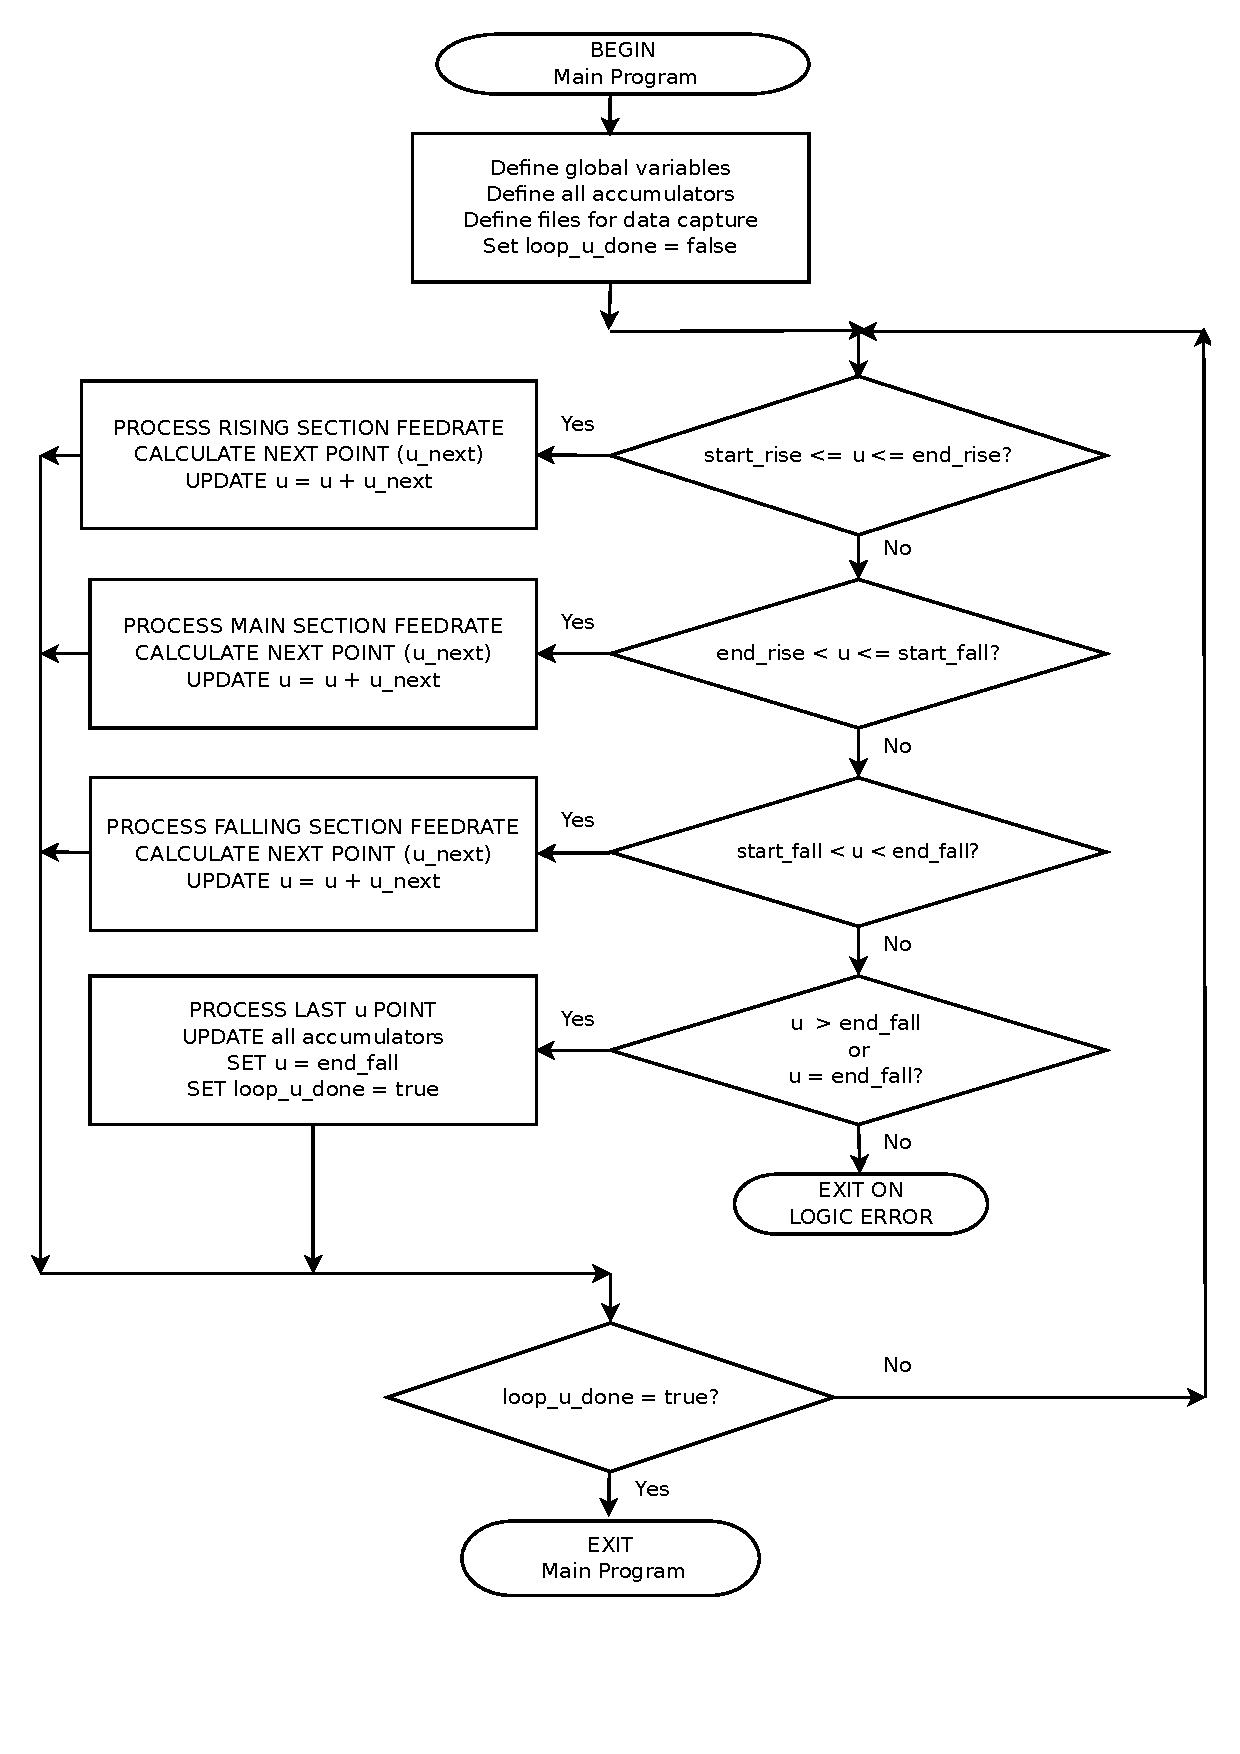
\includegraphics[width=1.15\textwidth,]{Images/Chap3/00-main-10-Main-Program-Algorithm.pdf} 
\end{figure}

%% =============================================
\clearpage
\pagebreak
\section{Feedrate Limit algorithm regions}

\noindent The flow chart for the main program shows that the range of processing is divided into 3 separate regions for $0.0 \le u \le 1.0$ as follows.
\begin{enumerate}
	\item Region ($start\_rise \le u \le end\_rise$), the feedrate rising S-curve region.
	\item Region ($end\_rise < u \le start\_fall$), the feedrate dynamic variation main region.
	\item Region ($start\_fall < u \le end\_fall$), the feedrate falling S-curve region.
\end{enumerate}

\noindent where $start\_rise = 0.0$ and $end\_fall = 1.0$ with ($end\_rise$ and $start\_fall$) user selected.\\ 

\noindent For all parametric curves considered, a large majority of computations for the interpolation algorithm occurs in the feedrate dynamic variation or main region. The feedrate profiles vary markedly from curve to curve.\\

The rising S-curve and falling S-curve sections are regions where the $feedrate\_limit$ are determined by the user assigned rising and falling sigmoid or S-curves. The $feedrate\_limit$ is assigned the exact value according to the rising or falling S-curves. The current or running feedrates are still computed to ensure that the chord-error and running feedrate constraints are observed. In this work, 4 different values of FCs were considered (FC = 10, 20, 30, 40). The execution results are provided in Chapter 4.\\ 

It is important to note that CaseA (Above) and CaseB (Below) are the conditions before processing. During processing, all $current\_feedrates$ are either "iteratively pushed-down" to below and very close to its $feedrate\_limit$, or "iteratively pushed-up" to below and very close to its $feedrate\_limit$. \\

Thus, it effectively means without exception, all $current\_feedrates$ running in operation are below the $feedrate\_limit$ throughout the traversal of the parametric curve. The execution results will be shown in Chapter 4. This condition is called "feedrate constrained", and is one of the main objectives of this thesis.


%% RISING FEEDRATE FLOWCHART
%% =============================================
\clearpage
\pagebreak

%% PERFECT INCLUDE PDF IN LATEX (AS ONE FULL PAGE)
\begin{figure}
	\caption{Flowchart of Feedrate Rising S-Curve}
	\label{01-Feedrate-Rising-Region-flowchart.pdf}
	\centering
	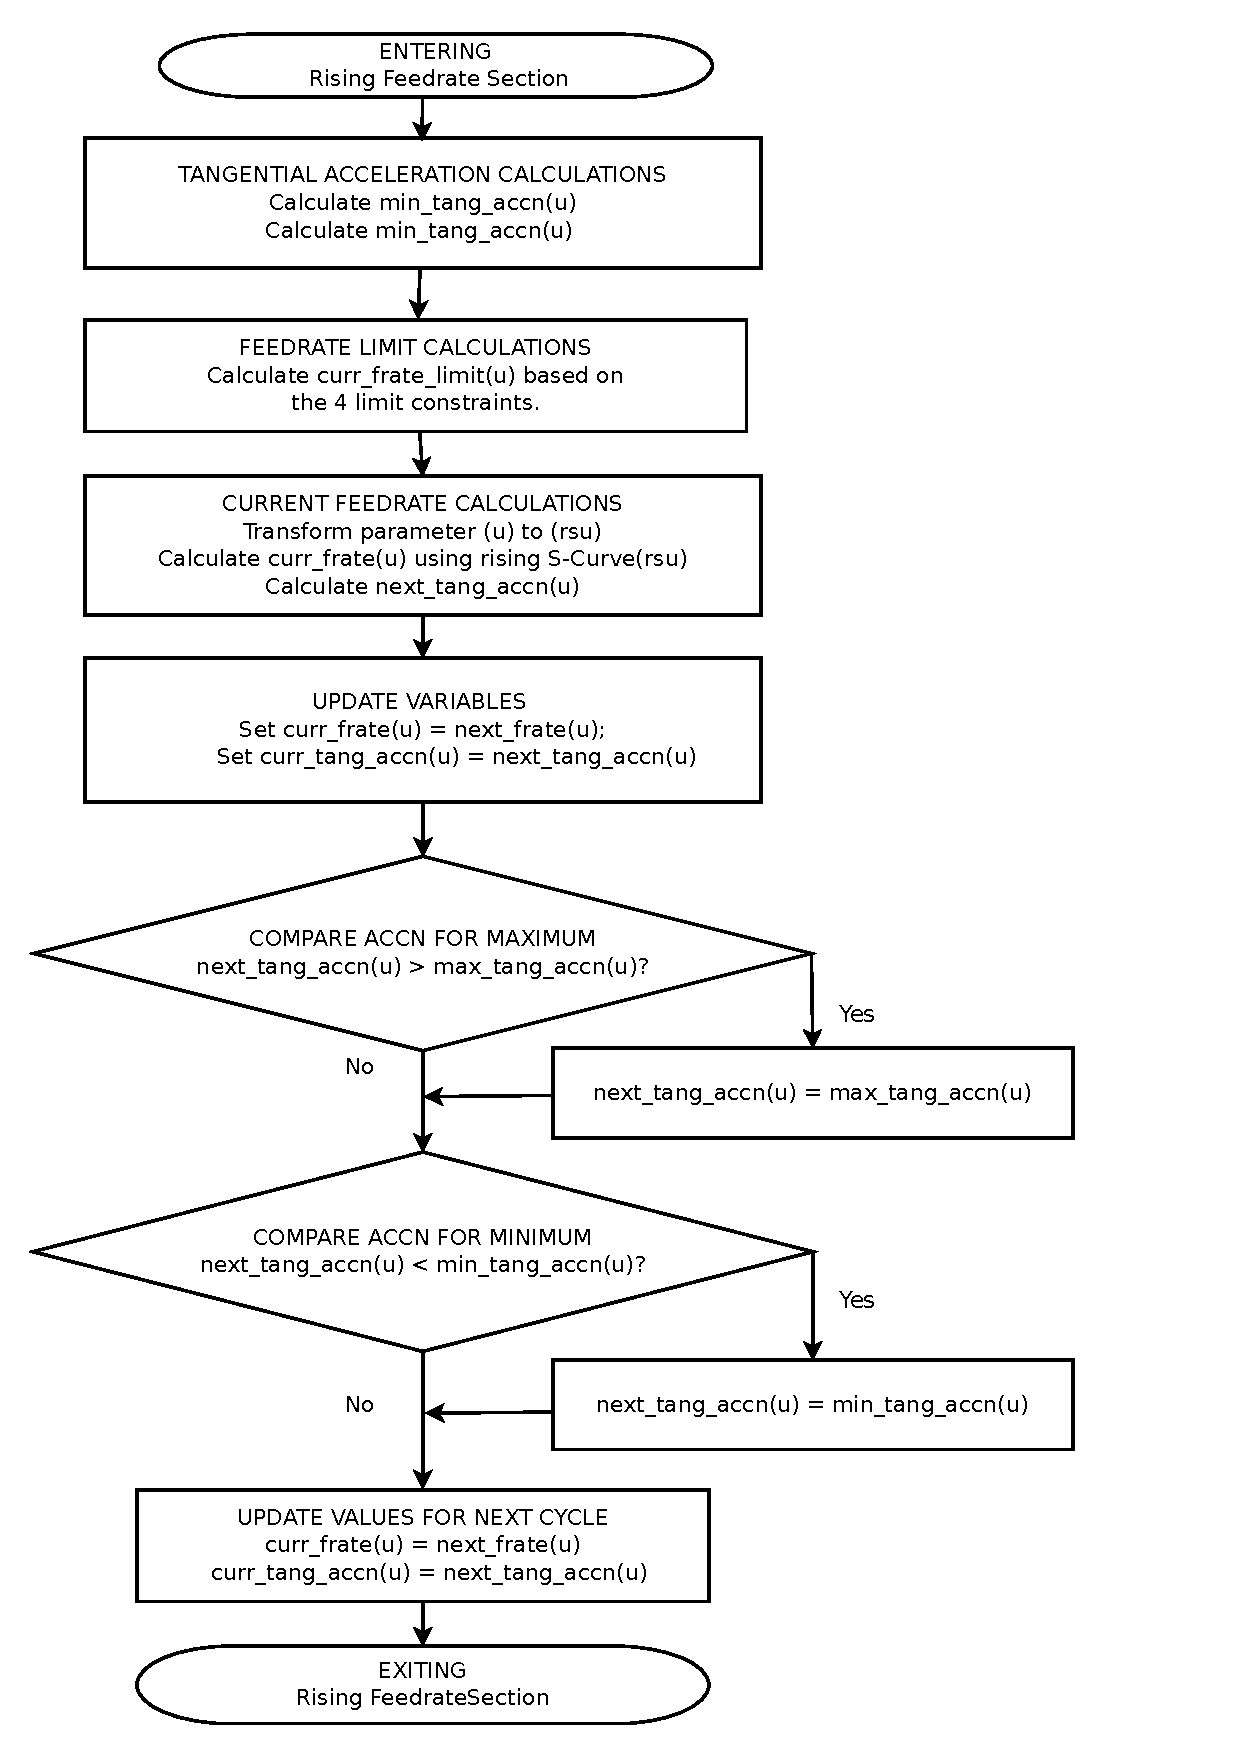
\includegraphics[width=1.10\textwidth,]{Images/Chap3/01-Feedrate-Rising-Region-flowchart.pdf} 
\end{figure}


%% FEEDRATE ABOVE FEEDRATE LIMIT PART 1/2
%% ==============================================
\clearpage
\pagebreak

%% PERFECT INCLUDE PDF IN LATEX (AS ONE FULL PAGE)
\begin{figure}
	\caption{Flowchart Current Feedrate above Feedrate Limit Part 1/2}
	\label{02-CaseA1-Feedrate-Above-Limit-Main-Region-flowchart.pdf}
	\centering
	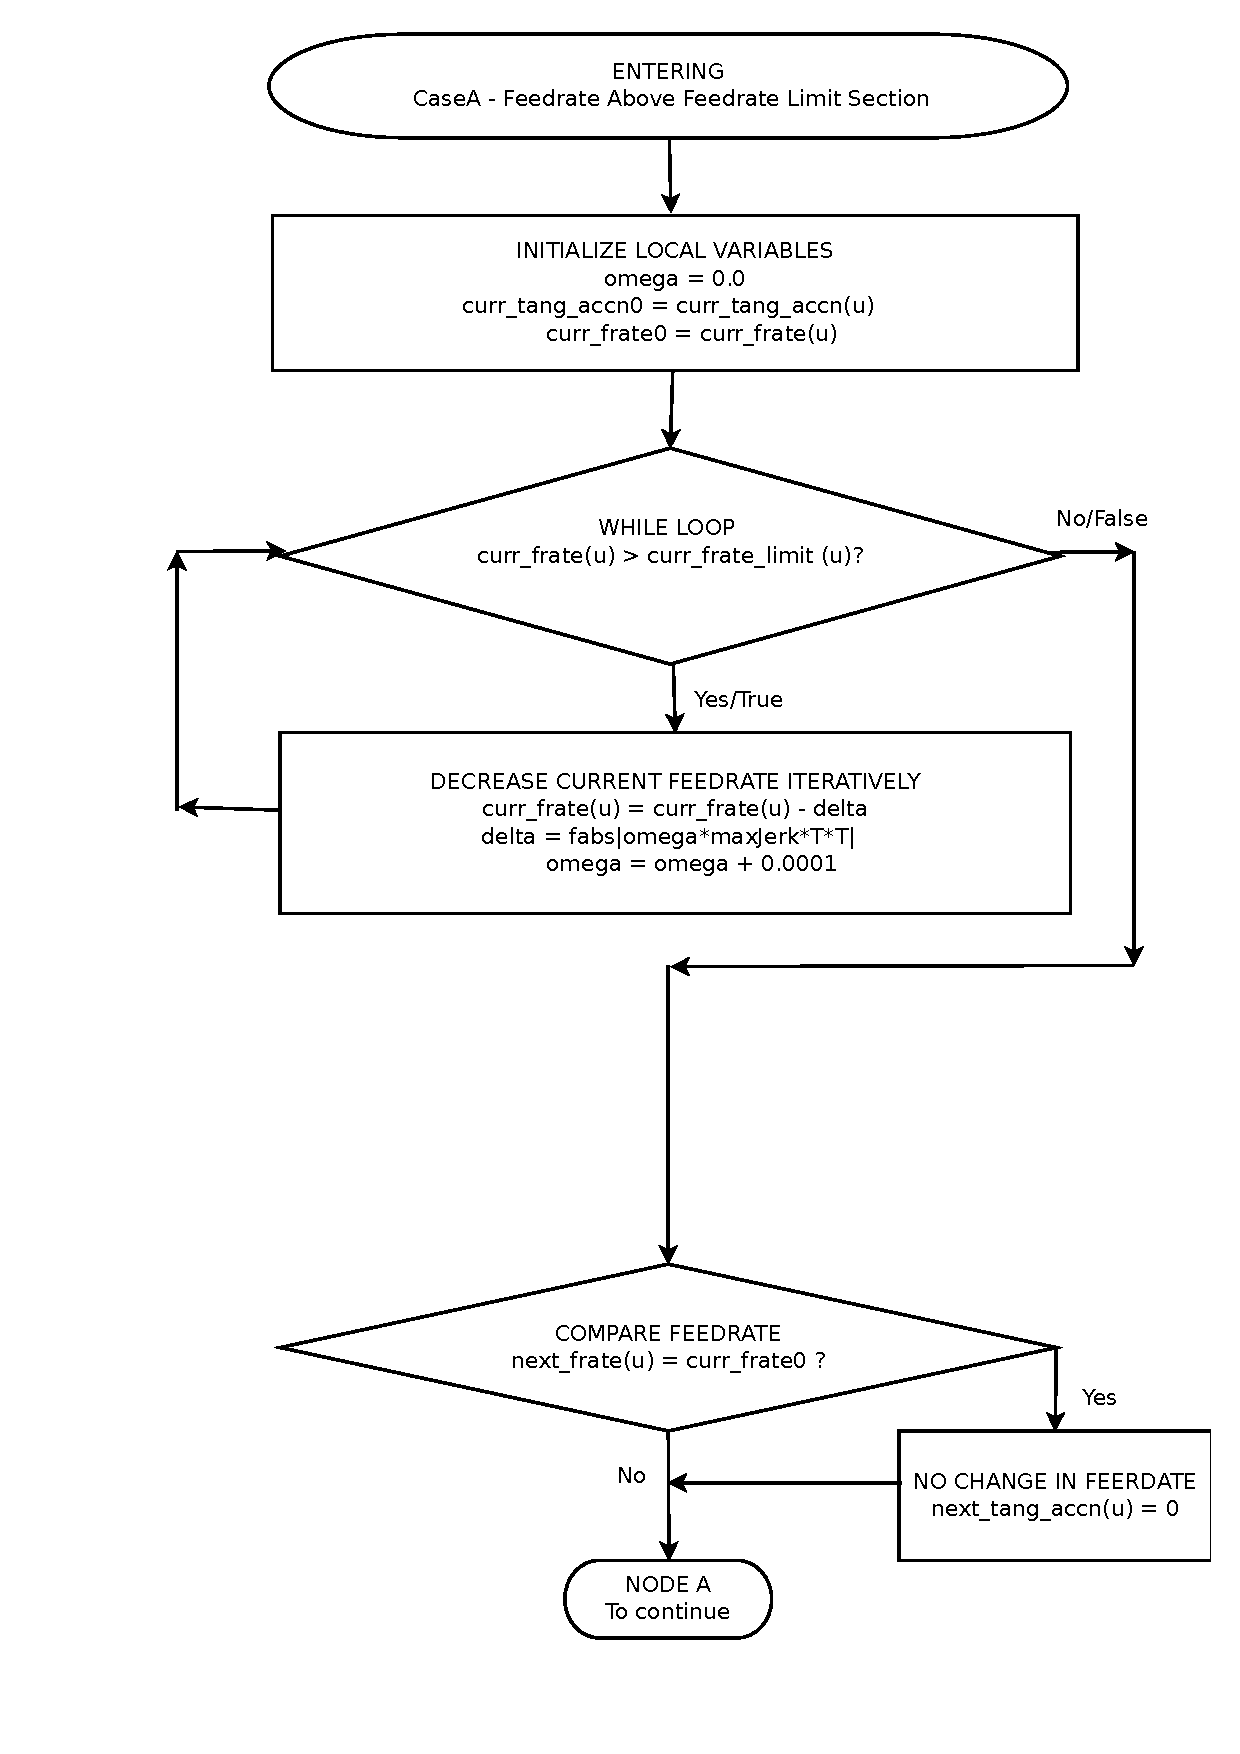
\includegraphics[width=1.10\textwidth,]{Images/Chap3/02-CaseA1-Feedrate-Above-Limit-Main-Region-flowchart.pdf} 
\end{figure}

%% FEEDRATE ABOVE FEEDRATE LIMIT PART 2/2
%% ==============================================
\clearpage
\pagebreak

%% PERFECT INCLUDE PDF IN LATEX (AS ONE FULL PAGE)
\begin{figure}
	\caption{Flowchart Current Feedrate above Feedrate Limit Part 2/2}
	\label{02-CaseA2-Feedrate-Above-Limit-Main-Region-flowchart.pdf}
	\centering
	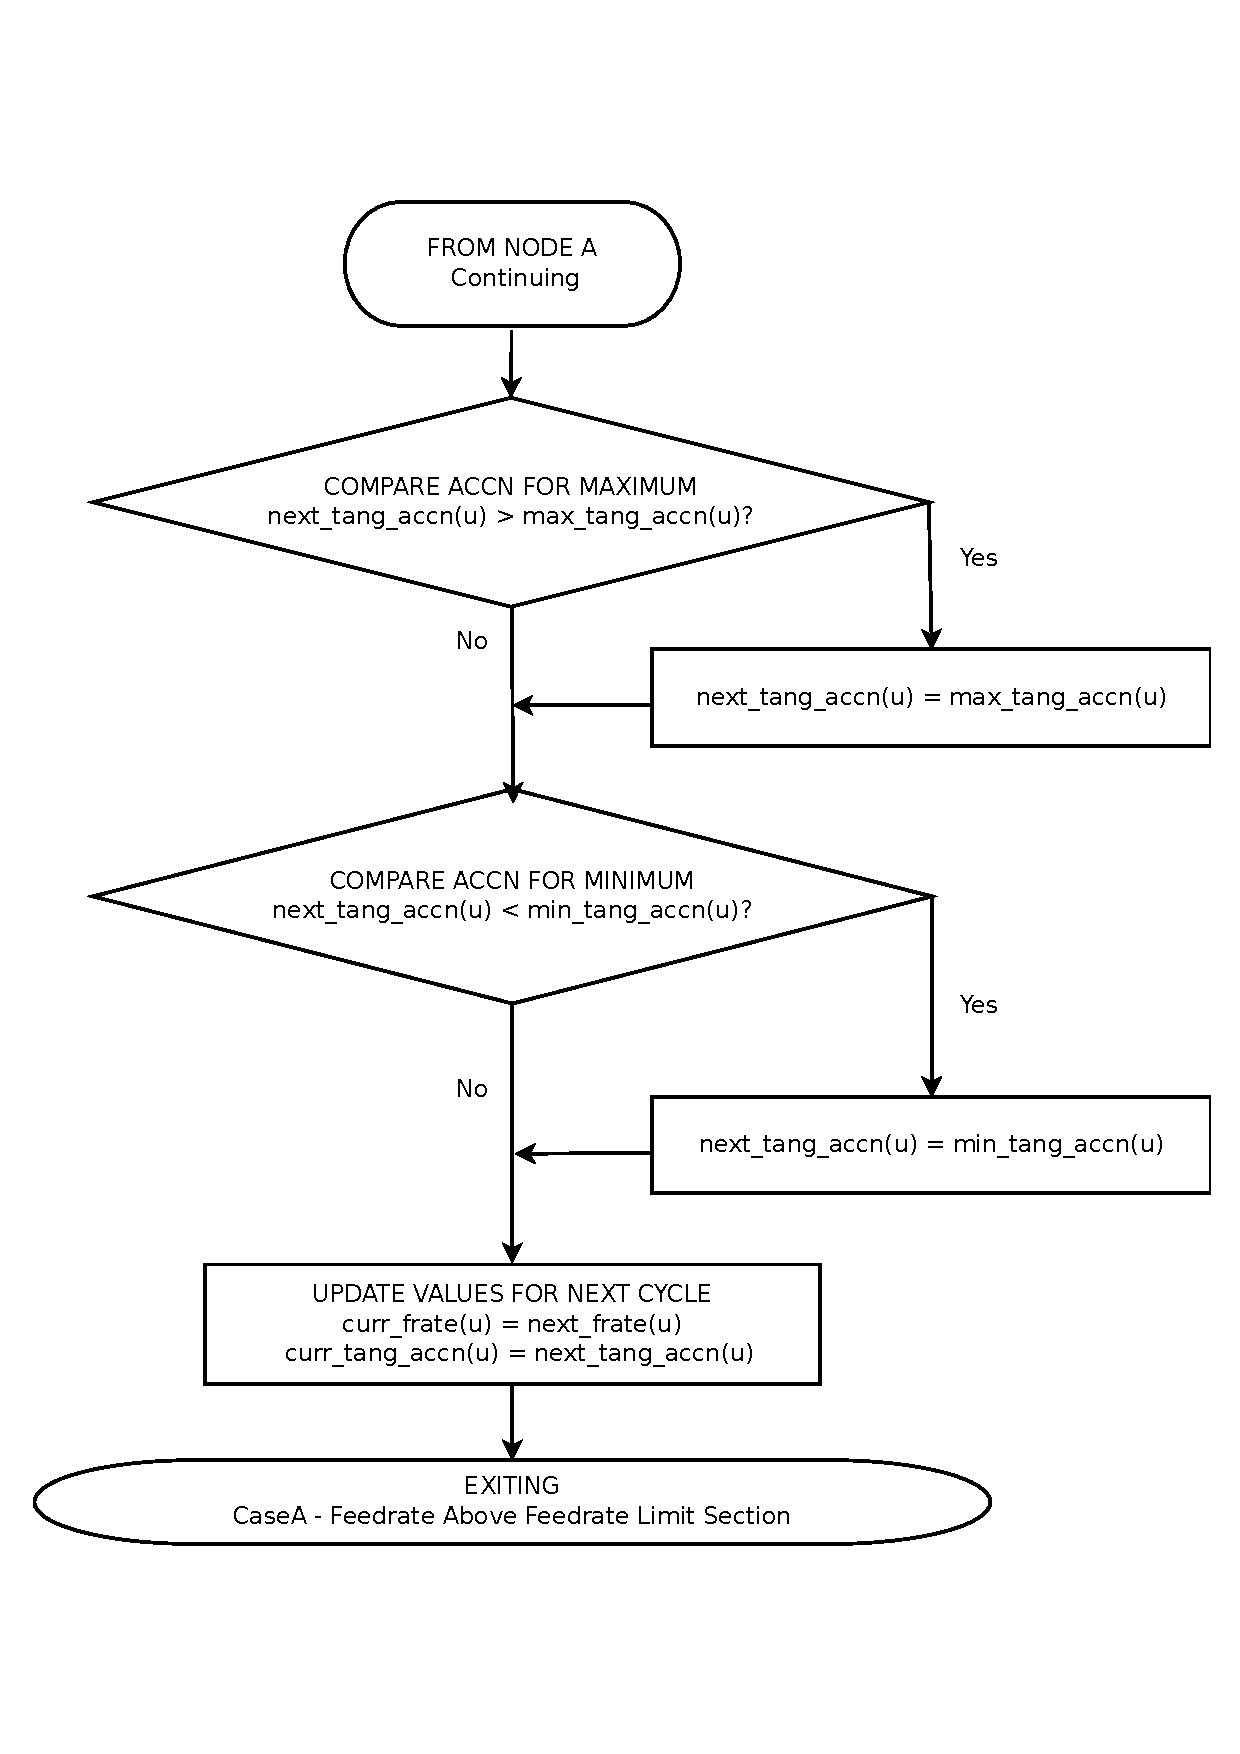
\includegraphics[width=1.10\textwidth,]{Images/Chap3/02-CaseA2-Feedrate-Above-Limit-Main-Region-flowchart.pdf} 
\end{figure}

%% FEEDRATE BELOW FEEDRATE LIMIT PART 1/2
%% =============================================
\clearpage
\pagebreak

%% PERFECT INCLUDE PDF IN LATEX (AS ONE FULL PAGE)
\begin{figure}
	\caption{Flowchart Current Feedrate below Feedrate Limit Part 1/2}
	\label{02-CaseB1-Feedrate-Below-Limit-Main-Region-flowchart.pdf}
	%% \centering
	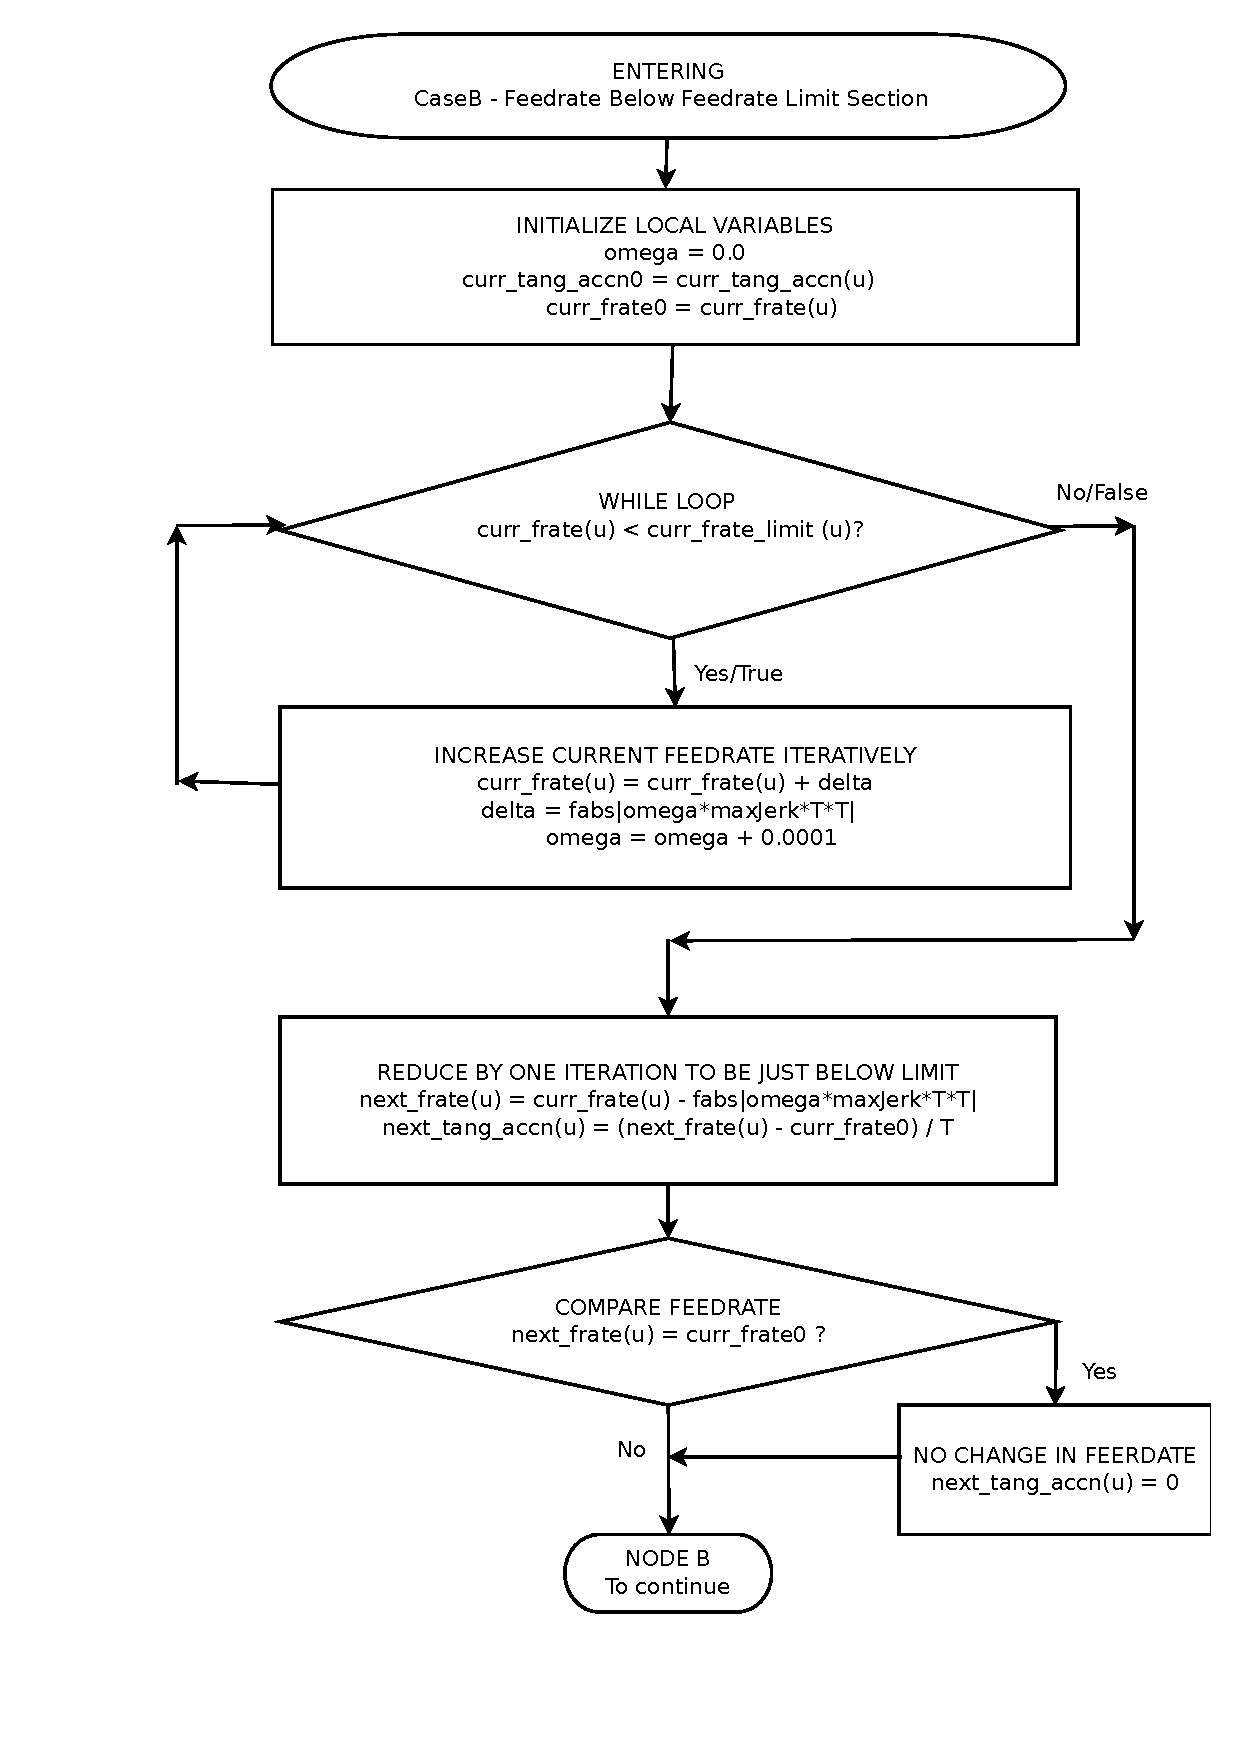
\includegraphics[width=1.10\textwidth,]{Images/Chap3/02-CaseB1-Feedrate-Below-Limit-Main-Region-flowchart.pdf} 
\end{figure}

%% FEEDRATE BELOW FEEDRATE LIMIT PART 2/2
%% =============================================
\clearpage
\pagebreak

%% PERFECT INCLUDE PDF IN LATEX (AS ONE FULL PAGE)
\begin{figure}
	\caption{Flowchart Current Feedrate below Feedrate Limit Part 2/2}
	\label{02-CaseB2-Feedrate-Below-Limit-Main-Region-flowchart.pdf}
	\centering
	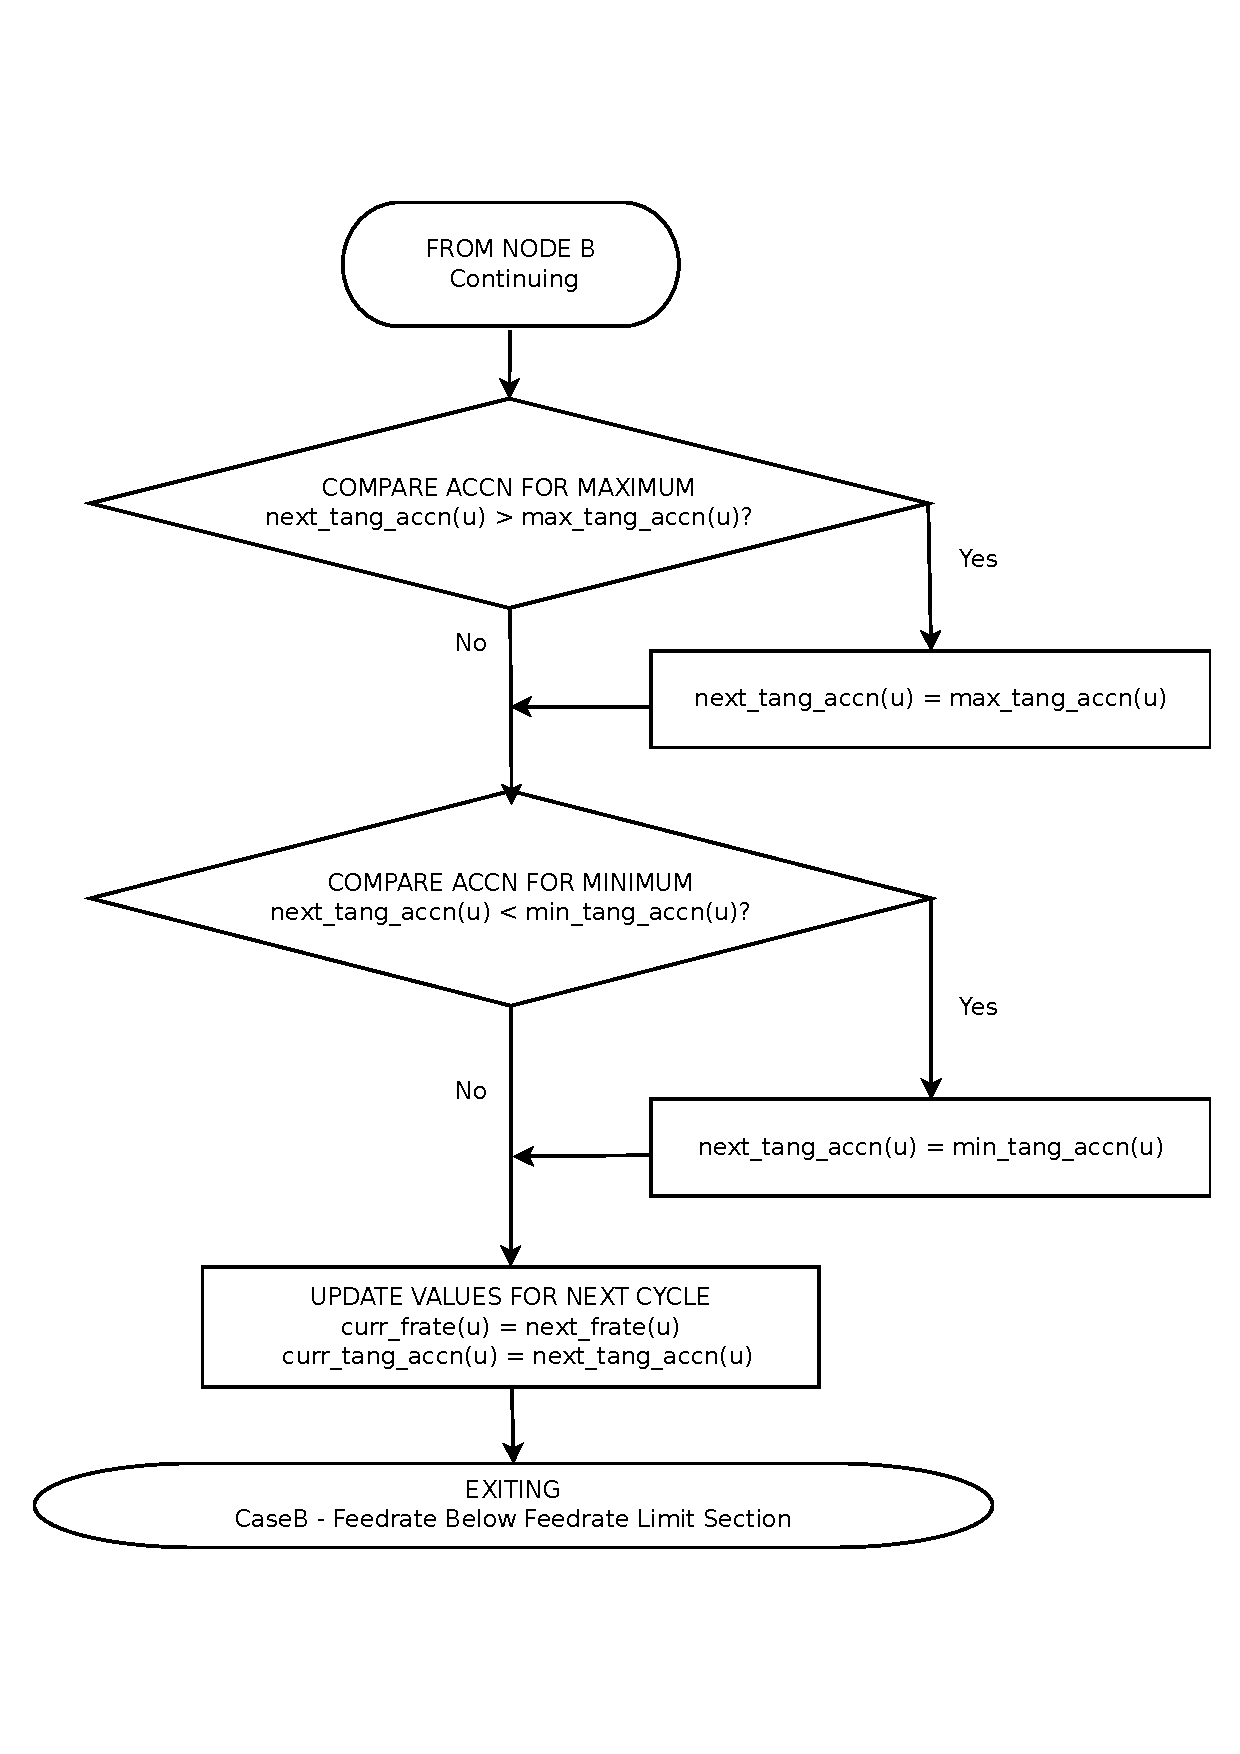
\includegraphics[width=1.10\textwidth,]{Images/Chap3/02-CaseB2-Feedrate-Below-Limit-Main-Region-flowchart.pdf} 
\end{figure}


%% FEEDRATE EQUAL LIMIT 
% =============================================
\clearpage
\pagebreak



%% PERFECT INCLUDE PDF IN LATEX (AS ONE FULL PAGE)
\begin{figure}
	\caption{Flowchart Current Feedrate equal Feedrate Limit}
	\label{02-CaseE-Feedrate-Equal-Limit-Main-Region-flowchart.pdf}
	\centering
	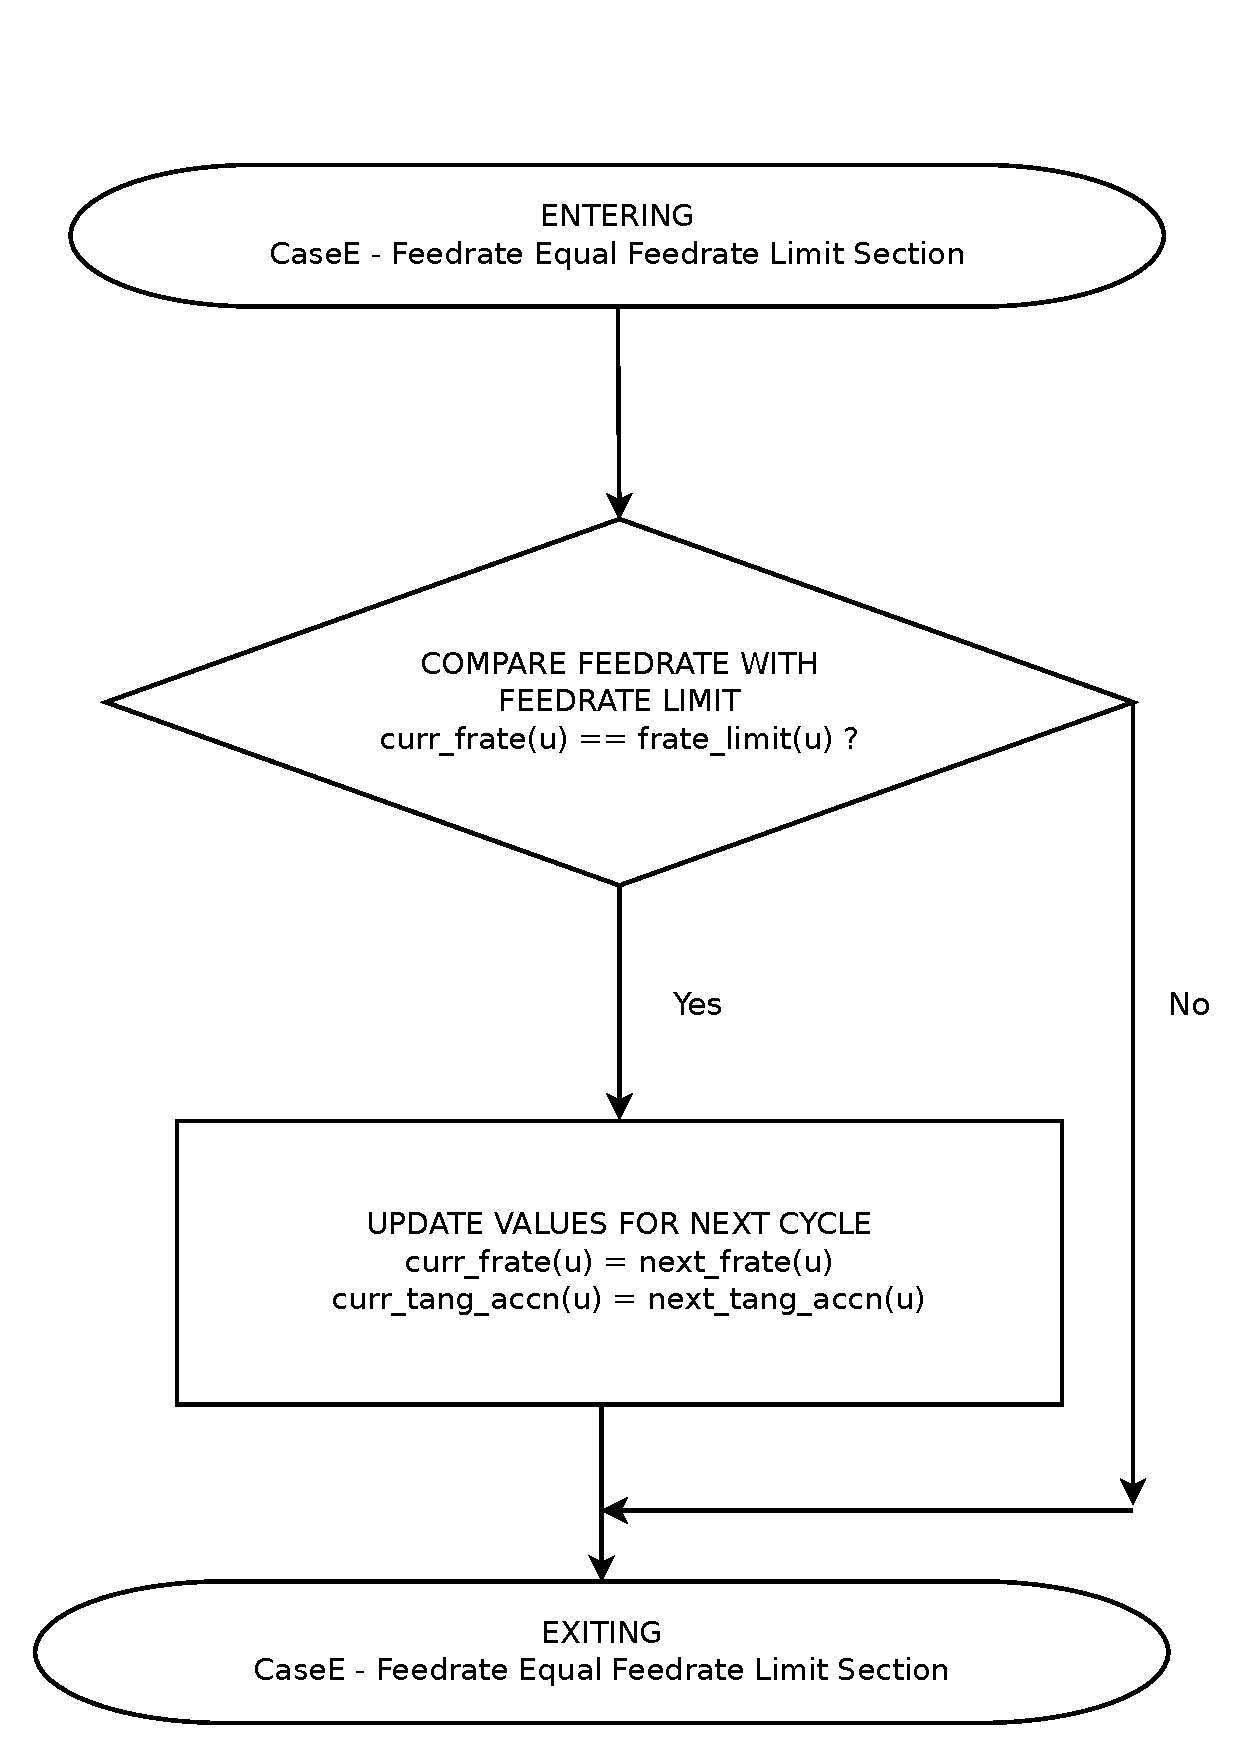
\includegraphics[width=0.85\textwidth,]{Images/Chap3/02-CaseE-Feedrate-Equal-Limit-Main-Region-flowchart.pdf} 
\end{figure}


%% CALCULATE U-NEXT 
%% =============================================
\clearpage
\pagebreak

%% PERFECT INCLUDE PDF IN LATEX (AS ONE FULL PAGE)
\begin{figure}
	\caption{Flowchart Calculate u\_next(u)}
	\label{04-Calculate-u-next-flowchart.pdf}
	%%\centering
	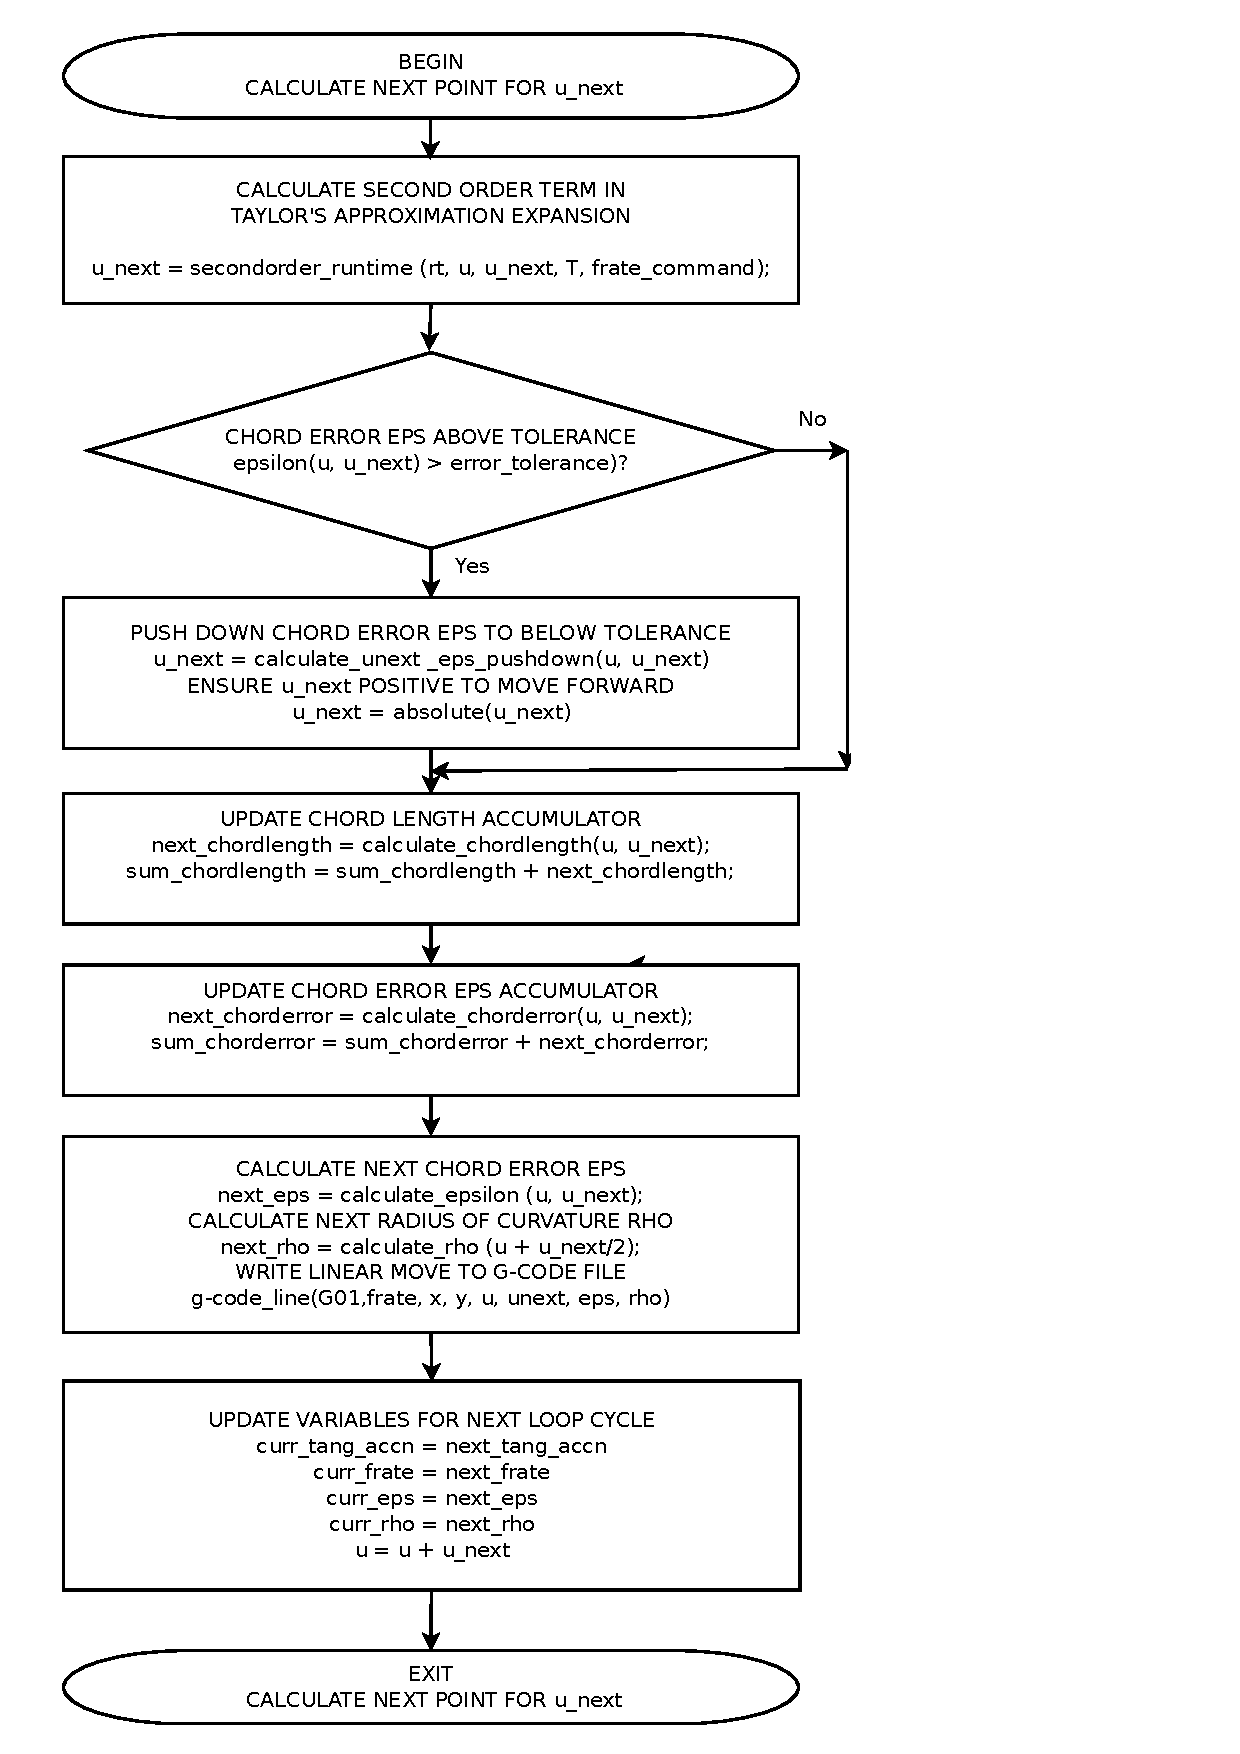
\includegraphics[width=1.10\textwidth,]{Images/Chap3/04-Calculate-u-next-flowchart.pdf} 
\end{figure}

%% =============================================
\clearpage
\pagebreak

\begin{figure}
	\caption{Flowchart Calculate u\_next(u) with eps pushdown}
	\label{05-Calculate-u-next-eps-pushdown-flowchart.pdf}
	%%\centering
	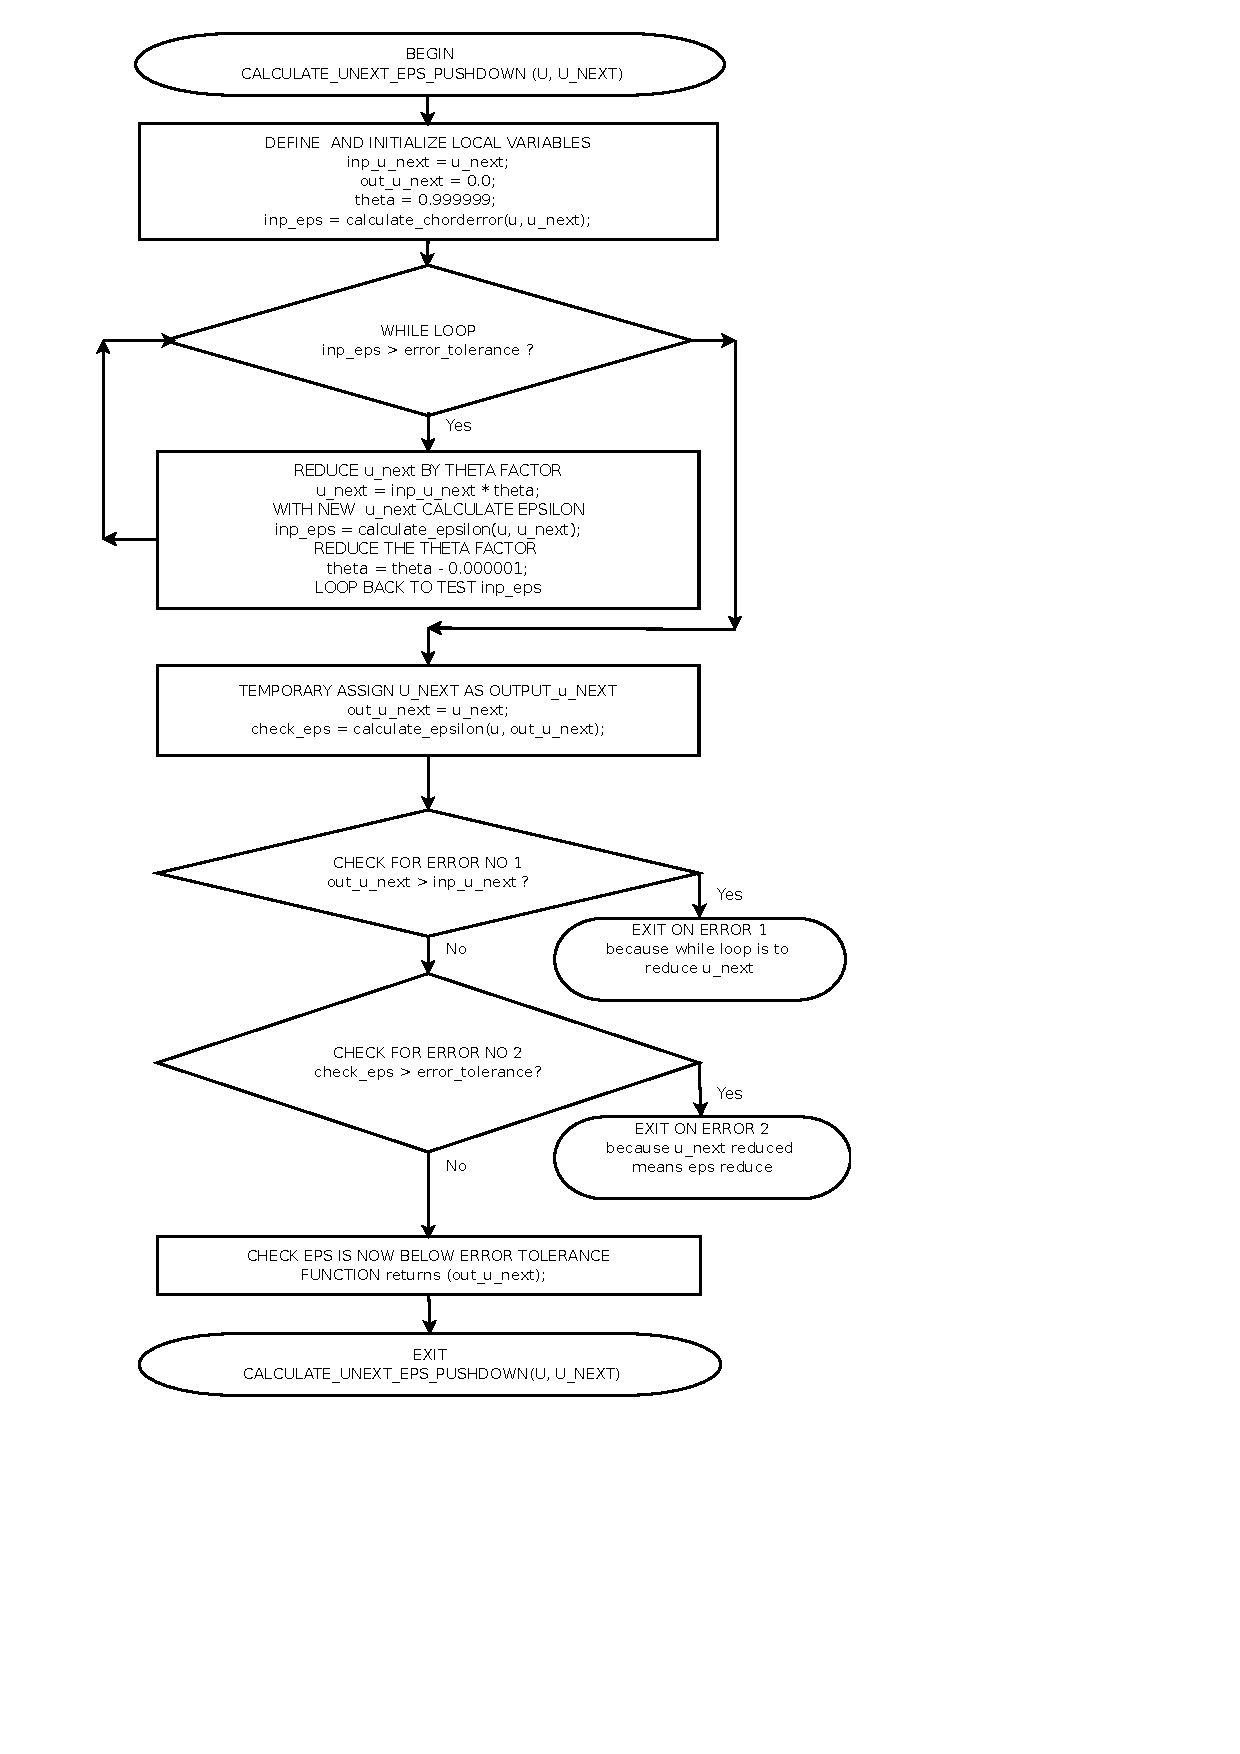
\includegraphics[width=1.40\textwidth,]{Images/Chap3/05-Calculate-u-next-eps-pushdown-flowchart.pdf} 
\end{figure}

%% FALLING FEEDRATE FLOWCHART
%% =============================================
\clearpage
\pagebreak

%% PERFECT INCLUDE PDF IN LATEX (AS ONE FULL PAGE)
\begin{figure}
	\caption{Flowchart of Feedrate Falling S-Curve}
	\label{03-Feedrate-Falling-Region-flowchart.pdf}
	\centering
	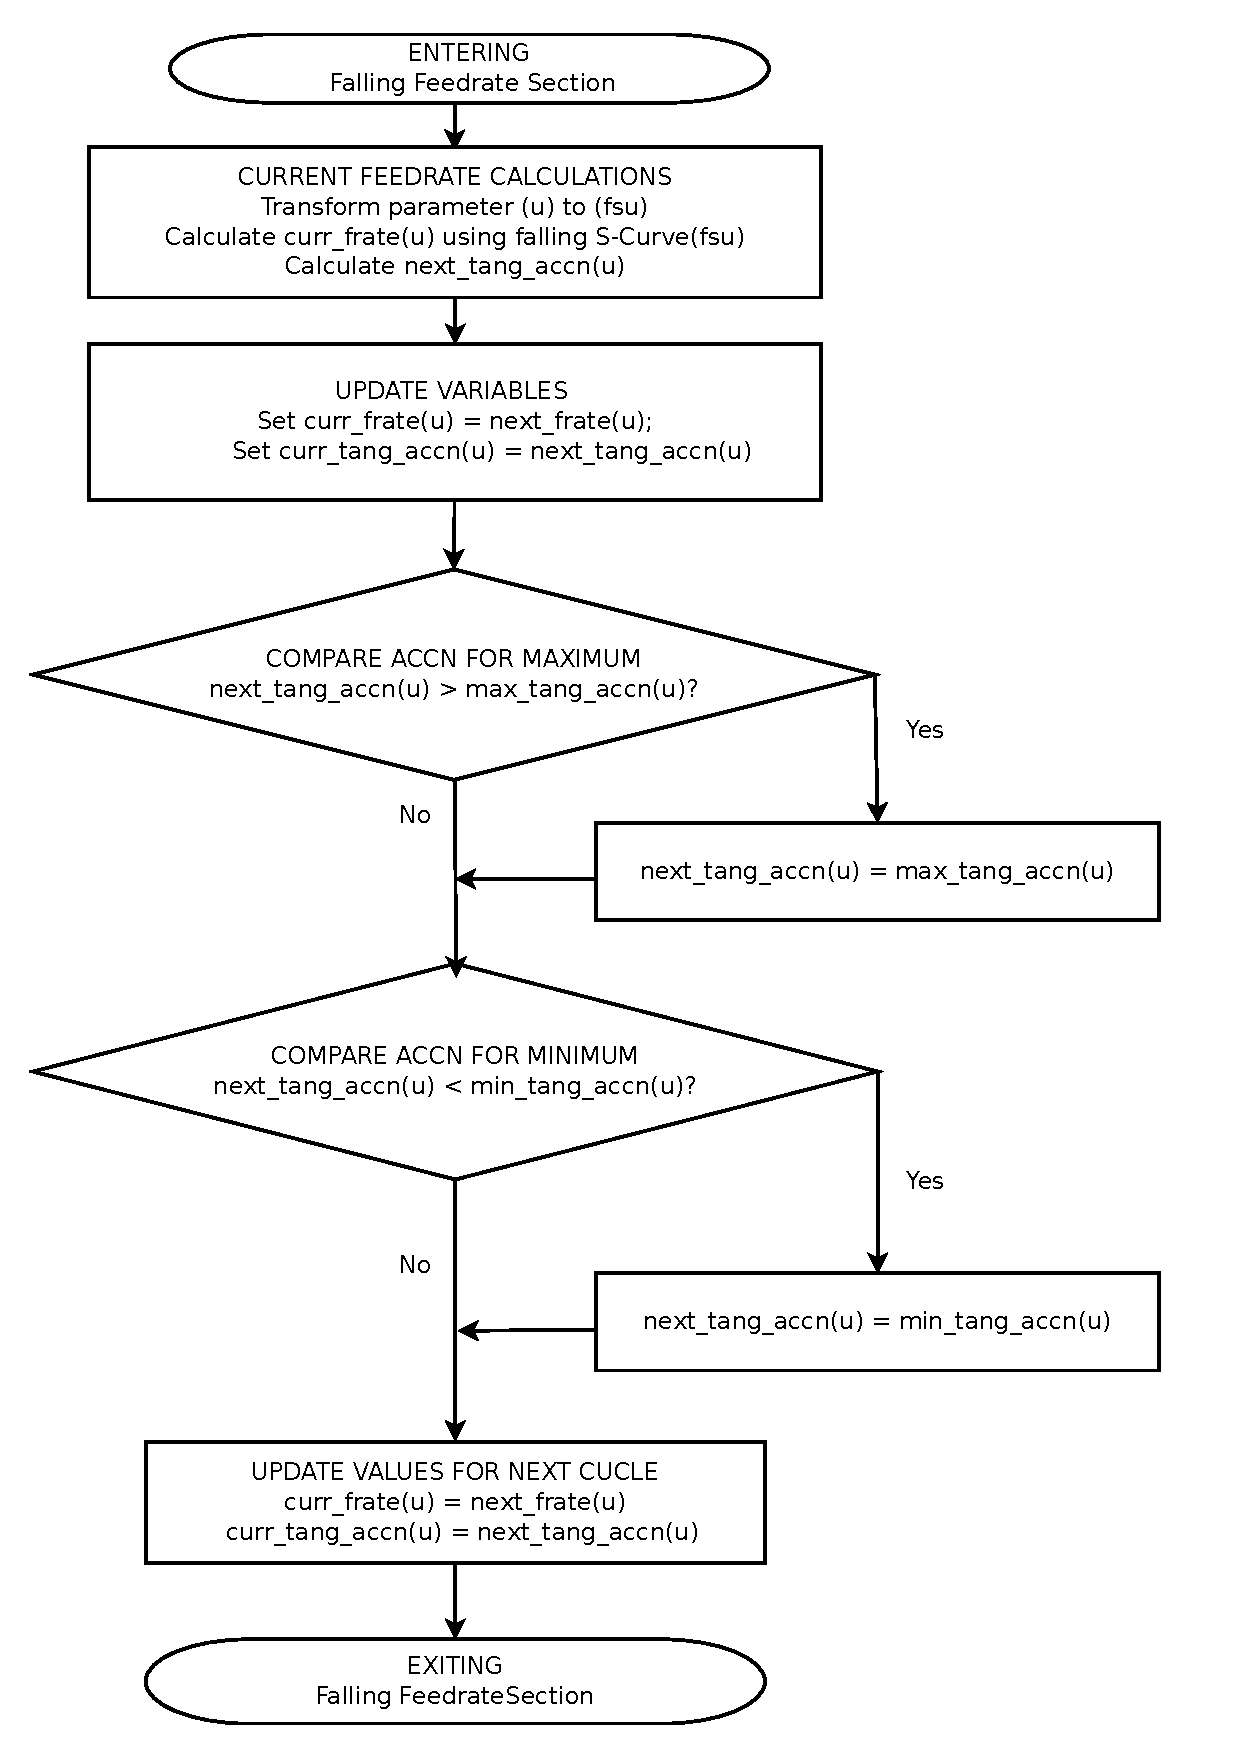
\includegraphics[width=1.10\textwidth,]{Images/Chap3/03-Feedrate-Falling-Region-flowchart.pdf} 
\end{figure}
%% 
%% ==============================================


% ======================================================
\clearpage
\pagebreak
\section{Feedrate falling S-curve}

The feedrate must not fall abruptly to zero. A smooth feedrate fall is required to ensure machine stability. The S-shaped curve below was selected for the fall of the current running feedrate to zero. \\

\[ curr\_frate(fsu) = 1 - \frac{curr\_frate\_limit(fsu)} { \Bigg( 1 + e^{(-fsu*fshape1)} \Bigg) ^{fshape2} }  \] \\

\noindent
where the applicable variable range is \\
$fsu\_start\_fall$ $\le$ $fsu$ $\le$ $fsu\_end\_fall$\\

\noindent
The linear parameter transformation from $u$ to $fsu$ is as follows:\\
$fsu$ = $fm*u$ + $fkonst$ \\

To ensure smoothness of the falling feedrate curves, simulations were conducted to determine the best values of the parameters.These variables are user specified.\\


\begin{table}[!ht]
	\begin{center}
		\caption{Falling S-curve parameters}
		\label{Falling-S-curve-parameters}	
		\begin{tabular}{ p{3.0cm} p{2.0cm} p{8.0cm}}
			\hline	
			fsu\_start\_fall & = 0.95  & beginning of falling S-curve \nonumber \\
			fsu\_end\_fall   & = 1.00  & end of falling S-curve \nonumber \\
			fshape1          & = 5.00  & S-curve smoothness shaping factor \nonumber \\
			fshape2          & = 8.00  & S-curve smoothness shaping factor \nonumber \\
			fsu1             & = 0.00  & start of u linear transformation\nonumber \\
			fsu2             & = 3.00  & end of u linear transformation \nonumber \\
			fm               & = calc  & slope calculated for each parametric curve \nonumber \\
			fkonst			 & = calc  & constant calculated for each parametric curve \nonumber \\ 
			fsu              & = calc  & transformed variable in the rising S-curve \nonumber \\
			\hline
		\end{tabular}
	\end{center}
\end{table}

%% ==============================================
\clearpage
\pagebreak

\section{Acceleration constraint lambda safety factor}

\begin{table}[ht]
	\begin{center}
		\begin{tabular}{ p{14.0cm} }
			\caption{Acceleration safety factor (lambda)}
			\begin{eqnarray}
            lamda  & = & user\_select\_safety\_factor(0.0 to 1.0)     \nonumber \\
%%	alphaVel(u) & = &  \Bigg | \frac { \Bigg (\odv{x(u)}{u} \Bigg) } { \sqrt { \Bigg( {\odv{x(u)}{u}} \Bigg )^{2} +  \Bigg ( {\odv{y(u)}{u}} \Bigg )^{2} } }  \Bigg |  \nonumber \\
%%	betaVel(u)  & = &  \Bigg | \frac { \Bigg (\odv{y(u)}{u} \Bigg) } { \sqrt { \Bigg( {\odv{x(u)}{u}} \Bigg )^{2} +  \Bigg ( {\odv{y(u)}{u}} \Bigg )^{2} } }  \Bigg |  \nonumber \\
			C & = & \sqrt {\frac{lamda*rho*xAcc_{max}} { \Bigg |(betaVel) \Bigg |} } \nonumber \\
			D & = & \sqrt {\frac{lamda*rho*yAcc_{max}} { \Bigg |(alphaVel)\Bigg |} } \nonumber \\
			fratelimit\_4 & = & minimum (C, D) \nonumber
			\end{eqnarray}
		\end{tabular}
	\end{center}
\end{table}

The $fratelimit\_4$ is about acceleration confinement within a (min, max) range of permissible accelerations. It is dependent on the combined dynamical and geometrical constraints. The dynamical machine constraints are in the maximum allowable axial accelerations of the machine as covered by $xAcc_{max}$ and $yAcc_{max}$. The geometrical constraints are in $alphaVel(u)$, $betaVel(u)$ and $rho(u)$, since $u$ changes along the curve these geometrical values also change. \\

The choice for the value of lambda, the safety factor for containment of acceleration, makes a big impact on the occurrence of jerks (jitters) in the feedrate. The values of 0.10, 0.18, 0.20 and 0.50 for lambda were tested for the algorithm runs to eliminate the jerks. A lower value of lambda will eliminate jerks but will reduce the feedrate significantly. The results for the threshold value for lamda is provided in Chapter 4 at reference link [\ref{chap4-Determination of acceptablel lamda}].

%% =============================================
\clearpage
\pagebreak

\section{Four(4) Algorithm Performance Metrics}

\noindent
There are four(4) metrics to assess the overall algorithm performance in this work. The first three terms are ratios while last term is
a percentage measure of the difference.

\begin{enumerate}
	\item SCE/TIP : This is the ratio of total sum-chord-error divided by the total number of interpolated points.  
	\item SCE/SCL : This is the ratio of total sum-chord-error divided by the total sum-chord-length.
	\item SAA/SCL : This is the ratio of the sum-arc-areas divided by the total sum-chord-length.
	\item 100(SAL-SCL)/SAL : This is the ratio of the difference between the sum-arc-length and the sum-chord-length, divided by the sum-arc	length and multiplied by 100 to represent it in percentage form. 
\end{enumerate} 

The calculation for the individual arc-length (AL) is provided in section [\ref{chap3-Arc-Length Approximate calculation}]. The calculation for the individual chord-length (CL) is provided in section [\ref{chap3-Chord-Length Exact calculation}]. The calculation for the individual arc-theta (AT) is provided in section [\ref{chap3-Arc-Theta Approximate calculation}]. The calculation for the individual arc-area (AA) is provided in section [\ref{chap3-Arc-Area Approximate calculation}]. \\

Consider these two(2) important terms. The term NAL(u) is the next-arc-length or length of the arc calculated by the algorithm from point u to the point u + (u next). Similarly, NCL(u) is the next-chord-length or length of the chord calculated by the algorithm from point u to the point u + (u next).\\

By definition, the sum-arc-length SAL(u), is the cumulative sum of NAL(u) from NAL(0.00) to NAL(u), where u is incremented by (u-next) in each step. Similarly, the sum-chord-length SCL(u), is the cumulative sum of NCL(u) from NCL(0.00) to NCL(u). Generally, we have the following definition of terms in this work.

\clearpage
\pagebreak

\begin{table}[ht]
%% \begin{center}

%% IMPORTANT TO SCALEBOX BELOW
\scalebox{0.90}{

\begin{tabular}{ p{16.0cm} }
\caption{Definitions of SAL(u), SCL(u), SAT(u), SAA(u) and SCE(u)}
\begin{eqnarray}
SAL(u) & = & \sum_{k=0.00}^{u}NAL(k) \nonumber  \\
SCL(u) & = & \sum_{k=0.00}^{u}NCL(k) \nonumber  \\
SAT(u) & = & \sum_{k=0.00}^{u}NAT(k) \nonumber  \\
SAA(u) & = & \sum_{k=0.00}^{u}NAA(k) \nonumber  \\
SCE(u) & = & \sum_{k=0.00}^{u}NCE(k) \nonumber  
\end{eqnarray}
\end{tabular}
%% \end{center}
}   %% IMPORTANT FOR SCALEBOX CLOSING
\end{table}


%% ===================================
\begin{table}[ht]
%% \begin{center}

%% IMPORTANT TO SCALEBOX BELOW
\scalebox{0.90}{

\begin{tabular}{ p{16.0cm} }
\caption{Definitions of Total SAL, Total SCL, Total SAT, Total SAA, and Total SCE}
\begin{eqnarray}
Total\_SAL & = & \sum_{k = 0.00}^{k = 1.00}NAL(k) \nonumber  \\
Total\_SCL & = & \sum_{k = 0.00}^{k = 1.00}NCL(k) \nonumber  \\
Total\_SAT & = & \sum_{k = 0.00}^{k = 1.00}NAT(k) \nonumber  \\
Total\_SAA & = & \sum_{k = 0.00}^{k = 1.00}NAA(k) \nonumber  \\
Total\_SCE & = & \sum_{k = 0.00}^{k = 1.00}NCE(k) \nonumber  
\end{eqnarray}
\end{tabular}
%% \end{center}

}   %% IMPORTANT FOR SCALEBOX CLOSING
\end{table}

\noindent
Note that the variable k is discrete and non-uniform. In fact, the successive values of k are exactly the successive values of u, generated by the interpolation algorithm, that is, while simultaneously constraining chord-error and running feedrate. \\

\noindent
Saying it is a straightforward manner, the values of k are exactly the values of the interpolated points u. That is the reason for k being non-uniformly spaced. Finding this k points is in fact, the main objective of the work in this thesis.

%% =============================================
\clearpage
\pagebreak

\subsection{Arc-Length Approximate calculation}
\label{chap3-Arc-Length Approximate calculation}

\begin{figure}
\caption    {Calculation for the Circle Arc-Length}
\label{chap3-Calculation for the Circle Arc-Length}
\centering
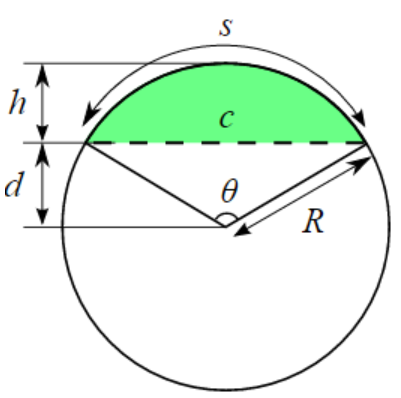
\includegraphics[width=0.60\textwidth,]{Chap3/images/Calculation-of-arc-segment-of-a-circle.png} 
\end{figure}

\noindent
The first-order approximation for the calculation of the arc-length $AL(u, u\_next)$ segment of a generic curve with equation C(x(u), y(u)), where x(u) and y(u) are known is given by:\\

\noindent
$ AL(u, u\_next) = (u\_next) * \sqrt{ {{\Bigg ( \odv{x}{u} \Bigg )^{2}} + {\Bigg ( \odv{y}{u} \Bigg )^{2} }} }  $  \\

\lstset{backgroundcolor=\color{white}, basicstyle=\linespread{1.00}\footnotesize, frame={topline, bottomline, leftline, rightline}}	
\begin{lstlisting}[caption={Implementation for Approximate Arc-Length Calculation}, label=lst-Implementation for Approximate Arc-Length Calculation]

// ==================================================================
double fxn_calc_arc_length(double u, double u_next)
// ==================================================================
{
  // LOCAL VARIABLES
  double arc_length = 0.0;
	
  // GEOMETRIC CALCULATION ARC LENGTH OF PARAMETRIC CURVES
  double dx_du = fxn_cvel_x(u);
  double dy_du = fxn_cvel_y(u);
  double sumsquare = (dx_du)*(dx_du) + (dy_du)*(dy_du);
  double arc_length0 = (u_next)*sqrt(sumsquare);
  arc_length = fabs(arc_length0);

  return (arc_length);
}
\end{lstlisting}


%% =============================================
\clearpage
\pagebreak

\subsection{Chord-Length Exact calculation}
\label{chap3-Chord-Length Exact calculation}

\noindent
The exact calculation for the chord-length $CL(u, u\_next)$ of a generic curve with equation C(x(u), y(u)), between two points on the curve at (x1, y1) and (x2, y2) is given by:\\

\noindent
$ CL(u, u\_next) = \sqrt{ \Bigg (x2-x1 \Bigg)^{2} + \Bigg (y2-y1 \Bigg )^{2}  } $ \\

\lstset{backgroundcolor=\color{white}, basicstyle=\linespread{1.00}\footnotesize, frame={topline, bottomline, leftline, rightline}}	
\begin{lstlisting}[caption={Implementation of Exact Chord-length Calculation}, label=lst-Implementation of Exact Chord-length Calculation]

// ==================================================================
double fxn_calc_chordlength_use_paramcurve (double u, double u_next)
// ==================================================================
{
  double chordlength;
  double x1, x2, y1, y2;
	
  // Use param curve and geometry
  x1 = fxn_cpos_x (u);
  y1 = fxn_cpos_y (u);
  x2 = fxn_cpos_x(u+u_next);
  y2 = fxn_cpos_y(u+u_next);
	
  // Pythagoras theorem for a right angled triangle
  chordlength = fabs(sqrt(pow((x2-x1), 2.0) + pow((y2-y1), 2.0)));
	
  return (chordlength); 
}
\end{lstlisting}


%% =============================================
\clearpage
\pagebreak

\subsection{Arc-Theta Approximate calculation}
\label{chap3-Arc-Theta Approximate calculation}

\noindent
The equation for the approximate arc-theta requires chord-length CL, and the radius of curvature rho values. The equation  used in this calculation is based on website reference [\href{https://www.engineersedge.com/math/circular_segment_equation_and_calculator__13796.htm}{circular\_segment\_equation\_and\_calculator}]. \\

$Arc\_Theta(CL, R) =  (2)*sin^{-1}(CL/2R) $\\

\noindent 
where R = approximately Radius of Curvature rho, and the chord-length CL is calculated from a previous equation.\\ 


\lstset{backgroundcolor=\color{white}, basicstyle=\linespread{1.00}\footnotesize, frame={topline, bottomline, leftline, rightline}}	
\begin{lstlisting}[caption={Implementation of Approximate Arc-Theta Calculation}, label=Implementation of Approximate Arc-Theta Calculation]

// ==================================================================
double fxn_calc_arc_theta(double u, double chord_length, double rho)
// ===================================================================
{
  double arc_theta = 0.0; 
  double arg_arcsine = chord_length/(2.0*rho);
	
  if ( (arg_arcsine < -1.0) || (arg_arcsine > +1.0) ) 
  {
    printf("ERROR: Angle_theta is out of range [-1.0 : +1.0] \n");
    printf("Value of angle arg_arcsine = %.12e \n", arg_arcsine );
    exit (1);
  } else {
    arc_theta = 2.0*asin(arg_arcsine);
  }
	
  return(arc_theta);
}
\end{lstlisting}

%% =============================================
\clearpage
\pagebreak

\subsection{Arc-Area Approximate calculation}
\label{chap3-Arc-Area Approximate calculation}


\noindent
The arc-area is the area bounded by the chord and the arc-segment. The equation for the approximate arc-area requires the radius of curvature rho and the angle theta in radians subtended by the arc segment. The equation  used in this calculation is based on website reference [\href{https://www.engineersedge.com/math/circular_segment_equation_and_calculator__13796.htm}{circular\_segment\_equation\_and\_calculator}]. \\

$Arc\_Area(R, theta) = (R^{2}/2)*(theta - sin(theta)) $\\

\noindent 
where R = approximately Radius of Curvature rho, and the subtended angle theta is in radians.\\ 


\lstset{backgroundcolor=\color{white}, basicstyle=\linespread{1.00}\footnotesize, frame={topline, bottomline, leftline, rightline}}	
\begin{lstlisting}[caption={Implementation of Approximate Arc-Area Calculation}, label=Implementation of Approximate Arc-Area Calculation]
	
// ==================================================================
double fxn_calc_arc_area(double u, double chord_length, double rho)
// ===================================================================
{
	double arc_area = 0.0;
	
	// GET VALUE OF ARC-THETA FROM PREVIOUS FUNCTION
	double arc_theta = fxn_calc_arc_theta(u, chord_length, rho);
	double DIFF = arc_theta - sin (arc_theta);

	// CALC ARC AREA
	arc_area = (rho*rho) * (DIFF)/2;
	
	return(arc_area);
}
\end{lstlisting}

%% =============================================

%% ==================================
\clearpage
\pagebreak

\section{Software engineering practice}
\label{sec-Software engineering practice}


The premise for the conduct of this thesis is to have a software design that is structured, fully functionalized and modularized. The use of GNAT Studio 2021 as the Integrated Development Environment (IDE) allows a combination of C, C++ and Ada code to be compiled together into a single executable. Ada is known for safe and secure codes and includes its own realtime library. \\

In general, software code implementations must not only run correctly, but must also run efficiently. Therefore, design of the codes must follow good software engineering practices. This thesis is under the category of mechatronics and systems design, so correct software codes is an important and critical part of the work. \\

The algorithm design must be highly structured, functionalized and modularized. This practice makes program execution flow readable and understandable. The resulting flowcharts will provide easy error tracing, adaptations, and additions of new functionality. \\
	
For example, inexperienced software programmers forget the simple rule that every time a function returns from a call, then all values of local variables are wiped out from memory. This requires that local variables be saved globally before the called function returns. This is a basic computing principle. \\
	
Technically, when a function executes, it may add some of its local state data to the top of the stack; when the function exits it is responsible for removing that data from the stack. In other words, since the stack memory of a function gets deallocated after the function returns, there is no guarantee that the value stored in those area will stay the same. References: \cite{Wikipedia:2023A} and \cite{Chen:2023}. \\
	
Another issue is the concept of zero in computing machines. In codes using floating-point representation of real numbers, any number below machine-epsilon (macheps), is treated as zero by the machine for addition and subtraction operations. Machine-epsilon is actually a very small but non-zero number, that varies from machine to machine. In the work conducted in this document at reference [App\ref{app4-Calculation of machine epsilon C code}], the machine-epsilon (macheps) for 64-bit double type was found to be  $2.22(10)^{-16}$. This means an algorithm check for addition or subtraction by zero is actually a check of addition or subtraction of very small non-zero numbers with values below machine-epsilon. Reference: \cite{Wikipedia:2023B}. \\
	
The side-effect phenomena in computing is another important issue. In computer science, an operation, function or expression is said to have a side effect if it modifies some state variable value(s) outside its local environment. This means, there are additional effects other than its primary effect of just returning a value to the caller of the operation. Because the algorithm in this work uses many global and local variables, it can be difficult to track changes and side-effects, that is, if the algorithm is not designed properly. Reference: \cite{Wikipedia:2023C}. \\
	
A decision operation (diamond flowchart symbol) must only have two outputs, True of False. It is a mistake, in fact a serious error not to have two branches as outputs. The algorithm must be designed to exit when there is an error at any point in its execution because all subsequent (downstream) calculations can be considered erroneous (useless) due to this upstream error. \\ 
	
Inclusion of error trapping functions is vital in any processing code. The algorithm in this work, for example, traps errors when $u\_next$ repeatedly stays at "zero" in five(5) consecutive loops in Taylor's expansion calculation. This means the interpolation step does not move forward to the next point. This is caused by the effect of machine epsilon. The "zero" here does not mean real zero, but is the computer machine-epsilon, the smallest non-zero value the computer can represent. Any value below this machine-epsilon is treated as zero for additions and subtractions by the computer. \\ 
	
Algorithm verification through accounting is the term used in this work to check that all calculations tally to the correct expected total value. As an example, the algorithm was built to check that the histogram total sum value (of interpolated points) tallies with the total number of interpolated points. Similarly, the histogram total sum value (of points above feedrate limit, and points below feedrate limit) tallies with the total number of interpolated points. In the same manner, the histogram total sum value (of points where chord-errors are all below tolerance) tallies with the total number of interpolated points.\\
	
In this work, the algorithm verification conducted above proves the achievement in simultaneously constraining chord-error and feedrates, thus meeting the objective of the interpolation algorithm.   \\


%% ==============================================================
%% MOVED FROM RESULTS CHAPTER
%% ==============================================================

\section{Design of Algorithm Codes}

\subsection{Algorithm Text Reports}

Every combination of the set (curve type, feedrate command FC and lamda safety factor) made as input to the algorithm will generate a summary report.\\

As examples, two(2) snippets of the summary report in this work for the Teardrop and Butterfly curves are provided in Listing [\ref{snp-Teardrop Algorithm Summary Output}] and Listing [\ref{snp-Butterfly Algorithm Summary Output}], respectively.\\

The snippet only shows Report No. 09 specifically on Algorithm Execution Statistics. There are eight(8) prior reports in the full report summary list for each execution run.\\




%% ========================================================
\clearpage
\pagebreak
%% \begin{landscape}

%% INPUT FROM FILE
%% \lstinputlisting[⟨key=value list⟩]{⟨file name⟩}
%% typesets the stand alone source code file as a displayed listing.
%% \lstset{backgroundcolor=\color{white}, basicstyle=\linespread{0.9}\scriptsize, frame={topline, bottomline, leftline, rightline}}

\lstset{backgroundcolor=\color{white}, basicstyle=\linespread{0.90}\footnotesize, frame={topline, bottomline, leftline, rightline}}	
\begin{lstlisting}[caption={Snippet of Teardrop Algorithm Summary Output}, label=snp-Teardrop Algorithm Summary Output]	
	
FC20-L0.18-A28-TEARDROP (REPORT NO. 09) ALGORITHM EXECUTION STATISTICS 	
	
TEARDROP TOTAL-INTERPOLATED-POINTS          	7.599000000000E+03
TEARDROP SUM-CHORD-ERROR-(mm)               	7.140807162860E-03
TEARDROP SUM-CHORD-ERROR/TOT-INTERPOL-PNTS  	9.398272128007E-07
	
TEARDROP SUM-ARC-LENGTH-(mm)                	1.018418663504E+02
TEARDROP SUM-CHORD-LENGTH-(mm)              	1.018418655699E+02
TEARDROP DIFF-ARC-LENGTH-CHORD-LENGTH-(mm)  	7.805327442156E-07
TEARDROP PCNT-DIFF-ARC-CHORD-LENGTH         	7.664163788301E-07
	
TEARDROP SUM-CHORD-ERROR/SUM-CHORD-LENGTH   	7.011661778683E-05
	
TEARDROP SUM-ARC-THETA-(rad)                	4.712268805770E+00
TEARDROP SUM-ARC-AREA-(mm2)                 	6.182290957317E-05
	
TEARDROP SUM-ARC-AREA/SUM-CHORD-LENGTH      	7.011661778683E-05
	
TEARDROP AVG-CHORD-ERROR-(mm)               	9.398272128007E-07
TEARDROP AVG-ARC-LENGTH-(mm)                	1.340377288107E-02
TEARDROP AVG-CHORD-LENGTH-(mm)              	1.340377277834E-02
TEARDROP AVG-ARC-THETA-(rad)                	6.201985793327E-04
TEARDROP AVG-ARC-AREA-(mm2)                 	8.136734610840E-09
	
2023-10-05 10:43:45	Program run duration   19.907344569 seconds. 
	
\end{lstlisting}
%% \end{landscape}

\lstset{backgroundcolor=\color{white}, basicstyle=\linespread{0.90}\footnotesize, frame={topline, bottomline, leftline, rightline}}	
\begin{lstlisting}[caption={Snippet of Butterfly Algorithm Summary Output}, label=snp-Butterfly Algorithm Summary Output]	
	
FC30-L0.18-A28-BUTTERFLY (REPORT NO. 09) ALGORITHM EXECUTION STATISTICS 		
	
BUTTERFLY TOTAL-INTERPOLATED-POINTS          	1.234300000000E+04	
BUTTERFLY SUM-CHORD-ERROR-(mm)               	4.846582536157E-03	
BUTTERFLY SUM-CHORD-ERROR/TOT-INTERPOL-PNTS  	3.926902071104E-07	
	
BUTTERFLY SUM-ARC-LENGTH-(mm)                	3.560730284349E+02	
BUTTERFLY SUM-CHORD-LENGTH-(mm)              	3.560727930088E+02	
BUTTERFLY DIFF-ARC-LENGTH-CHORD-LENGTH-(mm)  	2.354260789161E-04	
BUTTERFLY PCNT-DIFF-ARC-CHORD-LENGTH         	6.611735799000E-05	
	
BUTTERFLY SUM-CHORD-ERROR/SUM-CHORD-LENGTH   	1.361121273884E-05	
	
BUTTERFLY SUM-ARC-THETA-(rad)                	2.211618559661E+01	
BUTTERFLY SUM-ARC-AREA-(mm2)                 	1.298932073590E-03	
	
BUTTERFLY SUM-ARC-AREA/SUM-CHORD-LENGTH      	1.361121273884E-05	
	
BUTTERFLY AVG-CHORD-ERROR-(mm)               	3.926902071104E-07	
BUTTERFLY AVG-ARC-LENGTH-(mm)                	2.885051275603E-02	
BUTTERFLY AVG-CHORD-LENGTH-(mm)              	2.885049368083E-02	
BUTTERFLY AVG-ARC-THETA-(rad)                	1.791945032946E-03	
BUTTERFLY AVG-ARC-AREA-(mm2)                 	1.052448609294E-07	
	
2023-10-05 15:57:25	Program run duration    8.667691811 seconds. 
	
\end{lstlisting}
%% \end{landscape}

% ===================================
\clearpage
\pagebreak'
\subsection{Algorithm Functional Organization}


The functional organization of software codes for the realtime interpolation algorithm in this work is shown in Figure [\ref{img-Algorithm-Functional-Components}]. \\

The main algorithm in $src/algo$ comprises a series of seven(7) calculation modules, with the last module being the writing of RS272/NGC G-Code. The name of each code file is self-explanatory.\\

The $src/common$ and $src/cpp-codes$ folders are for local and imported code utilities commonly shared among the modules. The Integrated Development Environment (IDE) used in this work is capable of compiling C, C++ and Ada source codes combined into a single binary executable.\\

The $src/curves$ folder is where the ten(10) parametric curves in this work are located. The $src/files$ folder is the directory where all source codes to generate data and reports are located. This includes code to generate the G-Code file.\\

The $src/parallel\_pci$ and $src/parallel\_usb$ are the directories containing interface codes for the hardware parallel port on the computer. The former hardware is for PCI Parallel Card interface, while the later hardware is for USB-to-Parallel device interface.  \\

The $src/pthread$ folder is for multi-threading codes (C/C++ and Ada) while the $src/realtime$ folder is for Ada and C/C++ codes that implement realtime libraries. Note that Ada has its own built-in $Ada.Realtime$ library.\\

Multi-threading in Ada is called $Tasking$. Multi-threading for the algorithm in this project was tested successfully, however the overall execution is too slow and so was abandoned. It was found that the creation and destruction of new threads for runtime parameter at every u-loop is time-consuming. With that, the serial and sequential mode of processing was adopted for the algorithm.\\ 

The $src/reports$ folder is the storage location for all finished data and report files. The names of the files are meaningful like:
\singlespacing
\noindent $data\_calc\_frate\_limit.txt$,\\ 
$data\_calc\_intgrl\_error.txt$, \\
$data\_calc\_arclength\_chordlength.txt$,\\
$data\_calc\_tang\_accn.txt$,\\
$data\_calc\_time\_lookahead.txt$,\\ 
$data\_calc\_u\_next.txt$, \\
$data\_calc\_raw\_curve.txt$,
\doublespacing

\noindent and many more. Depending on the total number of interpolated points for the run, each file size typically ranges between one to 10 megabytes.\\ 

The $obj$ folder is the location of intermediate files during compilation, binding and linking. It is a system controlled folder and contains binary and semi-binary files. A snippet of the process of compilation, binding and linking is shown in Listing [\ref{snp-Snippet of Algorithm Compilation Binding and Linking}].\\

Finally, the $exec$ folder is where the single binary executable for the algorithm in this work is located. This binary executable is less than 100 kilobytes, and is considered very small.

% ===================================
\clearpage
\pagebreak'

%% NOTE: Limit is 0.55 of width	

\begin{figure}
	%% \centering
	\caption  {Algorithm-Functional-Components}
	\label{img-Algorithm-Functional-Components}
	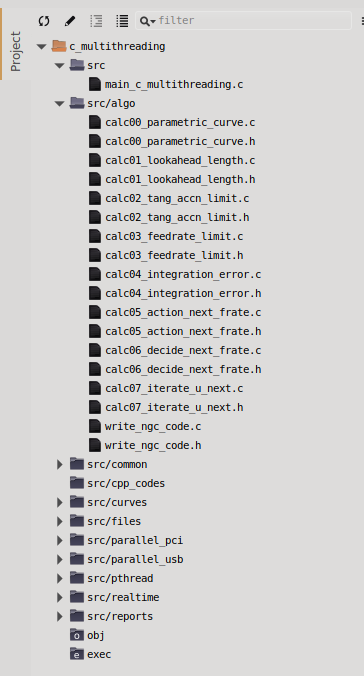
\includegraphics[width=0.55\textwidth]{Chap4/BW-Image-Algorithm-Functional-Components.png} 
\end{figure}

% ===================================
\clearpage
\pagebreak'

%% \begin{landscape}

%% INPUT FROM FILE
%% \lstinputlisting[⟨key=value list⟩]{⟨file name⟩}
%% typesets the stand alone source code file as a displayed listing.
%% \lstset{backgroundcolor=\color{white}, basicstyle=\linespread{0.9}\scriptsize, frame={topline, bottomline, leftline, rightline}}

\lstset{backgroundcolor=\color{white}, basicstyle=\linespread{0.92}\footnotesize, frame={topline, bottomline, leftline, rightline}}	
\begin{lstlisting}[caption={Snippet of Algorithm Compilation, Binding and Linking}, label=snp-Snippet of Algorithm Compilation Binding and Linking]	
	
gprbuild -d -P/home/wruslan/WRY-UMP-Thesis/
/Teadrop-FC20-Lamda018-Algo28-Codes/c_multithreading.gpr -s -k
	
Compile
[C]            main_c_multithreading.c
[C]            c_position.c
[C]            c_velocity.c
[C]            c_accelern.c
[C]            calc03_feedrate_limit.c
[C]            calc00_parametric_curve.c
[C]            calc06_decide_next_frate.c
[C]            calc07_iterate_u_next.c
[C]            write_ngc_code.c
[C]            calc05_action_next_frate.c
[C]            calc01_lookahead_length.c
[C]            calc02_tang_accn_limit.c
[C]            calc04_integration_error.c
[C]            preempt_rt.c
[C]            main_usb-to-parallel-port.c
[C]            usb_parallel_port.c
[C]            pci_parallel_port.c
[C]            c_report_01.c
[C]            test_threads_01.c
[C]            c_min_max_int_dbl_in_array.c
[C]            c_dtstamp.c
[C]            c_random_int_dbl.c
[C]            c_parallel_port.c
Link
[archive]      libc_multithreading.a
[index]        libc_multithreading.a
[link]         main_c_multithreading.c
[2023-10-10 11:06:29] process terminated successfully, time: 02.36s
	
\end{lstlisting}
%% \end{landscape}
%% ===================================


\clearpage
\pagebreak
\subsection{Algorithm and runtime parameters}\label{tab-Algorithm and runtime parameters}

The configuration of parameters in the realtime interpolation algorithm in this work is categorized into 3 sections, namely, the machine limits, the software runtime values, and the user specified runtime parameters. It is provided in Table [\ref{Algorithm and runtime parameters}] below. \\

\begin{table}[ht]
	%% \begin{center}
	\caption{Algorithm and runtime parameters}
	\label  {Algorithm and runtime parameters}
	%% IMPORTANT TO SCALEBOX BELOW
	\scalebox{0.90}{
		
		%% START COPY AND PASTE BELOW HERE
		%% FROM \begin{tabular} UNTIL \end{tabular)
		
		\begin{tabular}{ p{0.5cm} p{4.0cm} p{1.25cm} p{1.25cm} p{7.50cm} }
			\hline
			&                     &                 &       &     \\
			& MACHINE LIMITS      & VALUE  & UNIT   & DESCRIPTION \\
			%%	&                     &        &        &     \\
			1	&  x\_Vel\_max        & 30.0   & mm/s   & X-axis maximum velocity \\
			2	&  y\_Vel\_max        & 30.0   & mm/s   & Y-axis maximum velocity \\
			3	&  x\_Acc\_max        & 30.0   & mm/s2  & X-axis maximum acceleration\\
			4	&  y\_Acc\_max        & 30.0   & mm/s2  & y-axis maximum acceleration\\
			5	&  Jerk\_max          & 200.0  & mm/s2  & Maximum allowable jerk\\
			&                     &        &       &     \\
			& RUNTIME VALUES      &        &       &     \\
			%%	&                     &        &       &     \\
			1   & u\_end\_rise        &  0.05  & nil   & Rising S-curve range (0.0 .. 0.05)\\
			2   & rshape1             &  5.00  & nil   & Sigmoid curve rise shaping factor 1\\
			3   & rshape2             &  8.00  & nil   & Sigmoid curve rise shaping factor 2\\
			4   & u\_start\_fall      &  0.95  & nil   & Falling S-curve range (0.95 .. 1.00)\\   
			5   & fshape1             &  5.00  & nil   & Sigmoid curve fall shaping factor 1)\\
			6   & fshape2             &  8.00  & nil   & Sigmoid curve fall shaping factor 2)\\
			7	& T\_interpol         & 0.001  & s     & Interpolation time (period) \\
			&                     &        &       & 1 millisecond per step. \\
			8	& Error\_tol          & 1E-6   & mm    & Chord-error tolerance for  \\
			&                     &        &       & maximum allowable chord-error. \\
			9   & ngc\_scale          & 1.0    & nil   & RS274/NGC G-code scaling factor \\
			10	& ngc\_feedrate\_min  & 3.0    & mm/s  & Minimum NGC feedrate setting for\\
			&                     &        &       & startup and shutdown of CNC machine.\\
			11	& PI constant used    & PI     & nil   & PI = 3.14159\_26535\_89793\_238 precision\\
			&                     &        &       & at 18 decimal digits (from internet)\\
			&                     &        &       &     \\
			& RUN SPECIFIED       &Example &       &     \\
			%%	&                     &        &       &     \\
			1   & Curve selection     & AstEpi & nil   & Curve selected for algorithm to execute. \\
			&                     &        &       & Ten(10) different choices for this work. \\
			2   & Feedrate Command FC &  20.0  & mm/s  & Maximum feedrate set that should not \\
			&                     &        &       & be exceeded. For example: 10, 20, 30. \\
			3   & Lamda safety factor &  0.18  & nil   & Acceleration limit safety factor. \\
			&                     &        &       & A number between (0.0 .. 1.0) \\
			&                     &        &       &     
		\end{tabular}
		
		%% END COPY AND PASTE		
		
	}   %% IMPORTANT FOR SCALEBOX CLOSING
	\hrule
\end{table}

Note that the Feedrate Command (FC) is the value of the running feedrate that the user wants if it is following a straight line without any constraints. This is the user preferred feedrate. \\

The Feedrate Command is one of the four (4) components that determine the feedrate limit. The feedrate limit is dynamic, changes as parameter u changes, and is the minimum value among the four(4) components. The Feedrate Command is a user selected system constant. In the algorithm, the running feedrate is "forced and adjusted" to be as close to the feedrate limit throughout the parameter range.

%% ==============================================================
%% ==============================================================

\clearpage
\pagebreak

\section{Working environment setup}

The four(4) computing machines in this work comprise HP-Laptop-01, HP-Laptop-02, HP-Desktop-01 and HP-Desktop-02. The two laptops are identical in hardware specifications (HP brand, 8-CPU cores, 16 GB Memory, 1.5 TB SSD storage and so on). Similarly, the two desktops are also identical in hardware specifications (HP brand, 8-CPU cores, 16 GB Memory, 1.5 TB SSD storage and so on). The complete hardware specifications for the computing machines in this work are provided in Table [\ref{chap3-System Hardware Specifications}].\\

All four(4) computing machines are configured in a 3-way multiboot operating system. The user can select any one of the following operating systems: Linux Debian 10 Buster, Linux Ubuntu 20.04 LTS, or Microsoft Windows 10 Professional. The details are provided in Table [\ref{chap3-Operating Systems}].\\ 

All four(4) computing machines are installed with the same application software. This means the software installed are clones of each other. The details are provided in Table [\ref{chap3-Programming Software Languages}] for the programming languages, Table [\ref{chap3-Reporting Software Applications}] for the reporting software, and Table [\ref{chap3-Specialized Software Applications}] for the specialized software applications.\\

In the table for specialized software applications, the LinuxCNC-Axis software is the primary application to drive the CNC machine for all the G-codes generated in this work. The Panaterm application is used to communicate and monitor the status of the proprietary CNC-Servo drives responsible for control ofbthe CNC machine. The oscilloscope software, available for both Linux and Windows versions, are used to simultaneously trace 8-channels of digital or analog electrical signals. The CuteCom application is an RS232 serial communication software used drive and monitor serial signals in this work, including snooping, that is, a third party listening to RS232 serial communication between two serial devices. The DAQNavi Control Application is for Advantech products like PCIE-1884 DAQ card, and for user interface development using Qt6 C/C++ codes.\\    




%% ==============================================
\clearpage
\pagebreak

\section{System Hardware Environment}

\begin{table}[ht]
%%	\begin{center}
\caption{System Hardware Specifications}
\label{chap3-System Hardware Specifications}
\begin{tabular}{p{0.5cm} p{4.30cm} p{9.2cm} }
\hline	
\textbf{No} & \textbf{Category}   &    \textbf{Specification Description}\\
\hline
	&                       &    \\
1   &   HP-Laptop-01        & Model Hewlett-Packard, HP EliteBook 8570w \\
2	&   HP-Laptop-02        & Intel(R) Core(TM) i7-3630QM CPU @ 2.40GHz \\
	&                       & CPU Two Quad(4) cores, 64 bits, with 8 threads\\
	&                       & DDR3 16 GB System board memory, 1600 MHz clock\\
	&                       & System Caches: L1 32 KB, L2 256 KB, L3 6 MB\\
	&                       & SDDs: 1TB and 512GB Kingston Solid State Drives\\ 
	&                       & Display NVIDIA Corporation GK107GLM \\ 		
	&                       & GPU NVIDIA Corporation [Quadro K1000M]\\ 		
	&                       & Parallel parport0 PC-style 0x378 (0x778), irq 5\\
	&                       &    \\  
3   &	HP-Desktop-01       & Model Hewlett Packard EliteDesk 800 G1 TWR   \\
4   &	HP-Desktop-02       & Intel(R) Core(TM) i7-4790 CPU @ 3.60GHz \\  
	&                       & CPU Two Quad(4) cores, 64 bits, with 8 threads\\
	&                       & DDR3 18 GB System board memory, 1600 MHz clock\\
	&                       & System Caches: L1 256 KB, L2 1 MB, L3 8 MB\\
	&                       & SDDs: 1TB and 512GB Kingston Solid State Drives\\
	&                       & Display NVIDIA Corporation GK208 64bits 33Mhz\\ 
	&                       & GPU NVIDIA Corporation [GeForce GT 710B]\\         
	&                       & PCI parport0: PC-style 0xd100, irq 16 \\
	&                       & [PCSPP,TRISTATE]\\
	&                       & Advantech PCIE-1884 Signal processing card 32 bits\\
    &                       & \\
\hline
\end{tabular}

%% \hrule
%% \hline
%% \end{center}
\end{table}



%% ===============================================
\clearpage
\pagebreak
\section{Software Environment}

\subsection{Operating System}

\begin{table}[ht]
\caption{Operating Systems}
\label{chap3-Operating Systems}

\begin{tabular}{p{0.5cm} p{4.30cm} p{9.2cm} }
\hline	
\textbf{No} & \textbf{Category}   &    \textbf{Specification Description}\\
\hline
  &                       &    \\
1 & Ubuntu 20.04.6 LTS    & HP-Desktop-01 and 02, HP-Laptop-01 and 02\\
  &                       & Codename: focal, LSB version core-11.1 \\                   
  &                       & Kernel: linux-5.15.0-83-lowlatency \\
  &                       & SMP PREEMPT (2023) x86\_64 \\
  &                       & Preemptive Realtime OS, Symmetric Multi-Processor\\
  &                       &    \\  
2 &	Debian GNU/Linux 10   & HP-Desktop-01 and 02, HP-Laptop-01 and 02\\
  &                       & Codename: Buster   \\
  &                       & Kernel: 4.19.0-25-rt-amd64 x86\_64 GNU/Linux \\
  &                       & SMP PREEMPT RT Debian 4.19.289-2 (20230808) \\  
  &                       & Preemptive Realtime OS, Symmetric Multi-Processor\\
  &                       &    \\
3 & MS Windows 10 Pro     & HP-Desktop-01 and 02, HP-Laptop-01 and 02 \\
  &                       &    \\
  &                       &    \\
\hline
\end{tabular}  
\end{table}

%% ========================================  

\subsection{Programming Software Languages}  
  
\begin{table}[ht]
\caption{Programming Software Languages}
\label{chap3-Programming Software Languages}

\begin{tabular}{p{0.5cm} p{4.30cm} p{9.2cm} }
\hline	
\textbf{No} & \textbf{Category}   &    \textbf{Specification Description}\\
\hline
  &                       &    \\                    
1 &	C/C++, Ada            & GNAT Studio Community 2021 (20210423) \\ 
  &                       & GNAT 9.4.0 targeting x86\_64-linux-gnu   \\  
  &                       & SPARK Community 2021 (20210519)   \\    
  &                       &    \\
2  & GUI for C/C++         & Qt Creator 10.0.1 x86-64 \\
  &                       & Based on Qt 6.4.3 (GCC 10.3.1 20210422)   \\
  &                       & Built on May 04, 2023   \\
  &                       &    \\
3 &	Python                & Python 2.7.18 (Jul 1 2022), [GCC 9.4.0] on linux2\\
  &                       & Python 3.8.10 (May 26 2023), [GCC 9.4.0] on linux3\\
  &                       &    \\
4 &	Julia/Atom            & Julia Version 1.9.0 (2023-05-07)/Atom 1.58.0 x64 \\  
  &                       & \\
\hline
\end{tabular}  
\end{table}


%% ============================================
\clearpage
\pagebreak

\subsection{Reporting Software Applications}

\begin{table}[ht]
\caption{Reporting Software Applications}
\label{chap3-Reporting Software Applications}
	
\begin{tabular}{p{0.5cm} p{4.30cm} p{9.2cm} }
\hline	
\textbf{No} & \textbf{Category}   &    \textbf{Specification Description}\\
\hline
1 &	TeXstudio             & TeXstudio 3.0.1 (git n/a)  \\
  &                       & Using Qt Version 5.12.8, compiled with Qt 5.12.8 R   \\
  &                       &    \\
2 &	LibreOffice Suite     & Version: 6.4.7.2, Build ID: 1:6.4.7-0ubuntu0.20.04.8 \\
  &                       & CPU threads: 8; OS: Linux 5.15; UI VCL: gtk3; \\
  &                       &    \\ 
3 & Master PDF Editor     & Version 5, Build 5.7.60, 64 bit, (2021)  \\
  &                       & GCC: 5.3.1, GLIBC: 2.17, Qt: 5.9.5, SANE: 1.0.25  \\ 	
  &                       &    \\
4 &	Dia diagram editor    & Dia Version 0.97 + git (2011)\\
  &                       &    \\
5 & Gnuplot               & Gnuplot Version 5.2 patchlevel 8 (2019-12-01) \\ 
\hline
\end{tabular}
\end{table}

\subsection{Specialized Software Applications}

\begin{table}[ht]
\caption{Specialized Software Applications}
\label{chap3-Specialized Software Applications}
	
\begin{tabular}{p{0.5cm} p{4.30cm} p{9.2cm} }
\hline	
\textbf{No} & \textbf{Category}   &    \textbf{Specification Description}\\
\hline
1 &	CNC Control App       & LinuxCNC/Axis ver. 2.8.0 (2016)\\ 
  &                       & on Linux Debian 10 (Buster)  \\
  &                       &    \\
2 &	CNC Monitoring  App   & Panaterm version 4.5 (Panasonic)\\
  &                       & on Microsoft Windows 10 Pro \\
  &                       & \\
3 & Oscilloscope App      & Bitscope Digital Storage Oscilloscope (DSO) \\
  &                       & Linux - Version 2.8 Intel x86-64-bit \\ 	
  &                       & Windows - Version 2.8 Intel x86-64-bit \\   
  &                       &   \\ 
4 & Serial Communication  & CuteCom graphical serial terminal (RS232) \\ 
  & RS232 Snooper circuit & Linux GUI Version  0.30.3 (2015) \\
  &                       & Windows GUI Version  0.30.3 (2015)\\
  &                       &     \\
5 & DAQNavi Control App   & Advantech PCIE-1884 Data Acquisition Card \\ 
  &                       & Linux GUI Version  4.0.8.0 64-bit \\
  &                       & Windows GUI Version  4.0.8.0 64-bit\\  
 \hline
\end{tabular}
\end{table}

%% ==============================================
%% ==============================================
\clearpage
\pagebreak
\section{CNC System Setup}

The image of the CNC machine used in this work is shown in Figure [\ref{CNC-Research-Machine-3-Axis.jpg}]. The next Figure [	\ref{CNC-Research-Machine-3-Sets-Servo-Drives.jpg}] shows the three(3) Panasonic AC-Servo-Drives for the x, y, and z axes motions of the CNC machine. For this machine, the z-axis is used to move the pen tool up and down.\\ 

The next image shown in landscape mode in Figure [\ref{BHN-Validation-in-LinuxCNC-Axis-Screenshot.png}] illustrates the operations of the LinuxCNC-Axis software in driving the CNC machine to draw the diagram on its screen. The diagram to be drawn is represented by a G-code, a snippet of the code is provided in Listing [\ref{Link-to-Arabic-Calligraphy}]. \\

The image of the CNC system environment is shown in Figure [\ref{THE-FRONT-END-WhatsAppImage.jpeg}] and Figure [\ref{THE-BACK-END-WhatsAppImage.jpeg}]. \textit{Note: The images will be changed later.}\\


The overview of the CNC system environment is shown in Figure [\ref{Overview-CNC-system-environment.pdf}]. The multiplexed monitoring of the CNC Panaterm controller is shown in Figure [\ref{CNC-system-Panaterm-controller.pdf}]. The wiring diagram connections for parallel port, CNC servos and PCIE-1884-card is shown in Figure [\ref{Parport-CNC-servo-PCIE-1884-wiring-diagram.pdf}]. The snooper circuit for a third party computer to listen to RS232 serial communications between two devices is provided in Figure 	[\ref{RS232-Snooper-Circuit.pdf}].\\



%% ==============================================
\clearpage
\pagebreak

\begin{figure}
	\centering
	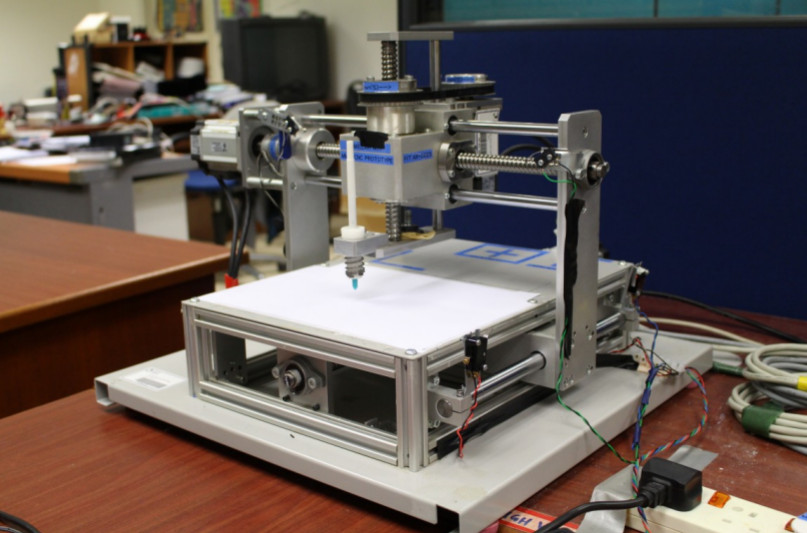
\includegraphics[width=1.00\textwidth]{Images/Chap4/CNC/CNC-Research-Machine-3-Axis.jpg} 
	\caption{The prototype 3-axis CNC research machine}
	\label{CNC-Research-Machine-3-Axis.jpg}
\end{figure}

\begin{figure}
	\centering
	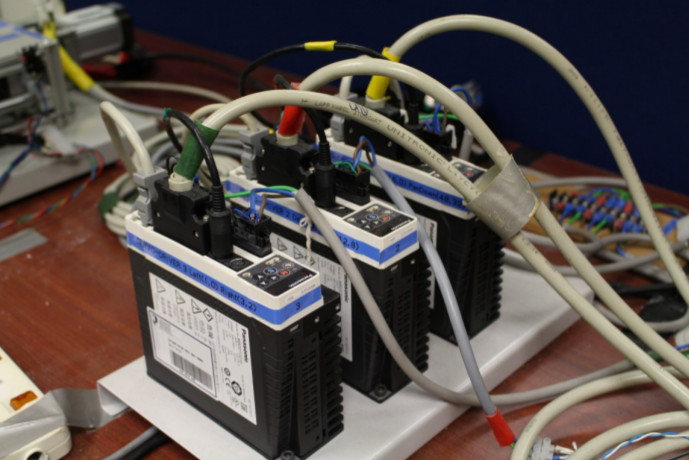
\includegraphics[width=1.00\textwidth]{Images/Chap4/CNC/CNC-Research-Machine-3-Sets-Servo-Drives.jpg} 
	\caption{The 3-sets AC servo drivers for the CNC research machine}
	\label{CNC-Research-Machine-3-Sets-Servo-Drives.jpg}
\end{figure}

%% LANDSCAPE LINUXCNC AXIS
%% ==============================
\clearpage
\pagebreak
\begin{landscape}
	\begin{figure}
	\caption{Validation of G-code using LinuxCNC Axis software}	
	\label{BHN-Validation-in-LinuxCNC-Axis-Screenshot.png}		
	\centering
	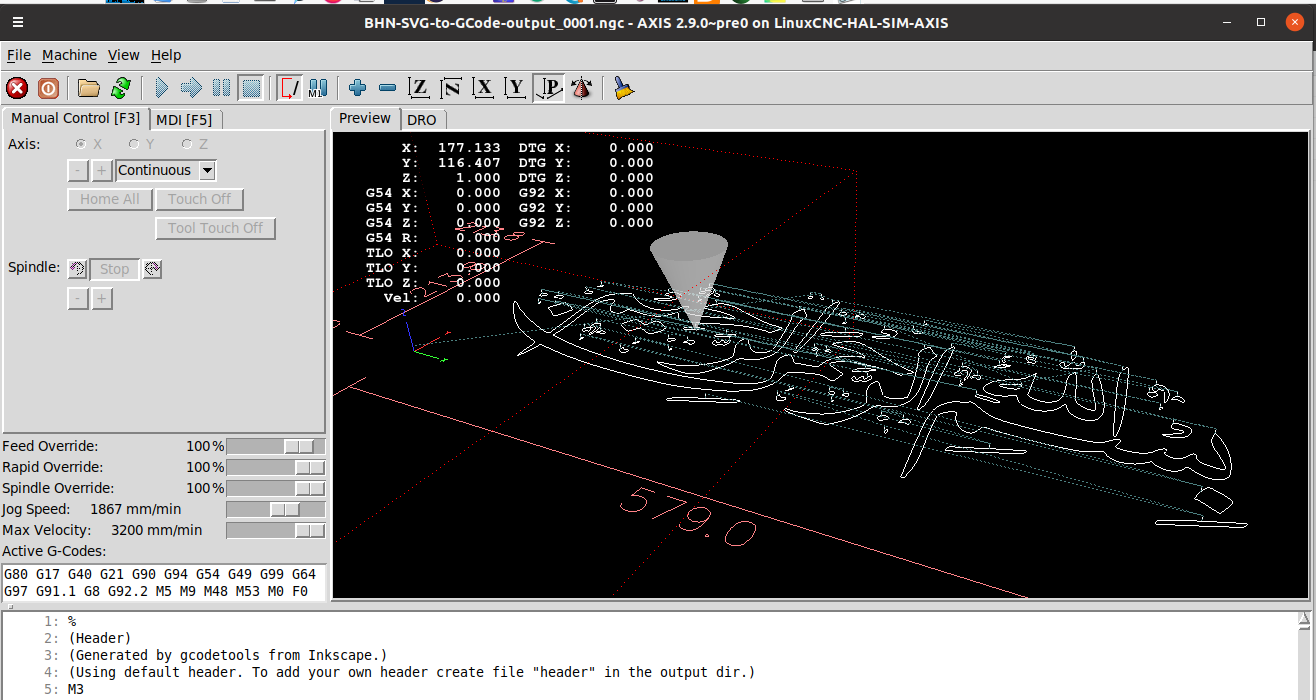
\includegraphics[width=1.70\textwidth]{Chap2/Images/BHN-Validation-in-LinuxCNC-Axis-Screenshot.png} 
	\end{figure}
\end{landscape}


% LISTING
%% ==============================
\clearpage
\pagebreak
\begin{landscape}
	
%% INPUT FROM FILE
%% \lstinputlisting[⟨key=value list⟩]{⟨file name⟩}
%% typesets the stand alone source code file as a displayed listing.
%% \lstset{backgroundcolor=\color{white}, basicstyle=\linespread{0.9}\scriptsize, frame={topline, bottomline, leftline, rightline}}
	
\lstset{backgroundcolor=\color{white}, basicstyle=\linespread{0.92}\footnotesize, frame={topline, bottomline, leftline, rightline}}	
\begin{lstlisting}[caption={G-code snippet for Arabic calligraphy}, label=Link-to-Arabic-Calligraphy]	
(Header)
(Generated by gcodetools from Inkscape.) 
(Using default header. To add your own header create file "header" in the output dir.)
M3
(Header end.)
G21 (All units in mm)
(Start cutting path id: path11762)
(Change tool to Default tool)
G00 Z5.000000
G00 X235.600000 Y35.100000
G01 Z1.000000 F100.0(Penetrate)
G03 X213.627800 Y25.129879 Z1.000000 I60.683117 J-162.930013 F400.000000
G03 X212.000000 Y22.400000 Z1.000000 I1.475151 J-2.729879
G03 X212.577899 Y21.936846 Z1.000000 I0.474545 J-0.000000
G03 X218.800000 Y23.900000 Z1.000000 I-8.264838 J37.036796
G02 X225.555826 Y26.585083 Z1.000000 I199.253827 J-491.492772
G02 X241.000000 Y32.500000 Z1.000000 I527.010173 J-1352.932266
G03 X257.708311 Y40.036826 Z1.000000 I-45.059557 J122.180722
G03 X259.000000 Y42.200000 Z1.000000 I-1.165476 J2.163174
G03 X258.293460 Y42.724778 Z1.000000 I-0.548158 J0.000000
G03 X235.600000 Y35.100000 Z1.000000 I111.496791 J-369.428872
G01 X235.600000 Y35.100000 Z1.000000
G00 Z5.000000
....
\end{lstlisting}
%% } %% END SCALEBOX

\end{landscape}
	
%% FRONT END ENVIRONMENT
%% ==============================
\clearpage
\pagebreak

\begin{landscape}
\begin{figure}
%%	\centering
\caption{The front end environment of the system}
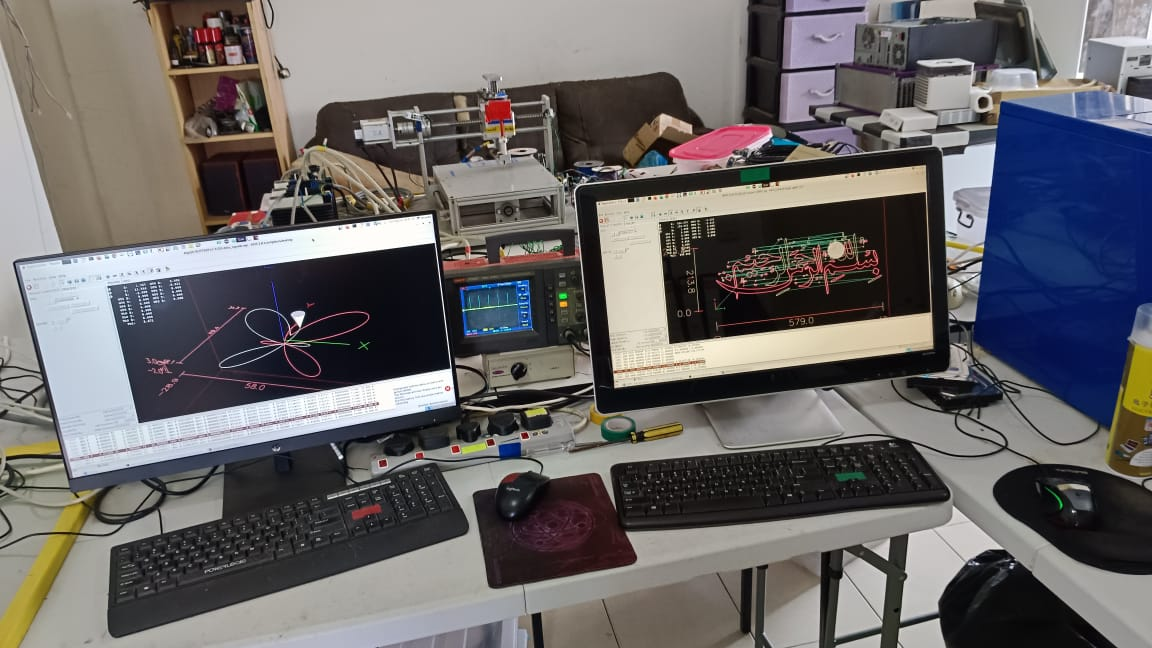
\includegraphics[width=1.60\textwidth]{Image0/THE-FRONT-END-WhatsAppImage.jpeg} 
\label{THE-FRONT-END-WhatsAppImage.jpeg}
\end{figure}
\end{landscape}

%% BACK END ENVIRONMENT
%% ==============================
%%\clearpage
%%\pagebreak
%%\begin{landscape}
%%	\begin{figure}
	%%	\centering
%%		\caption{TEMPORARY - The back end environment of the system}
%%		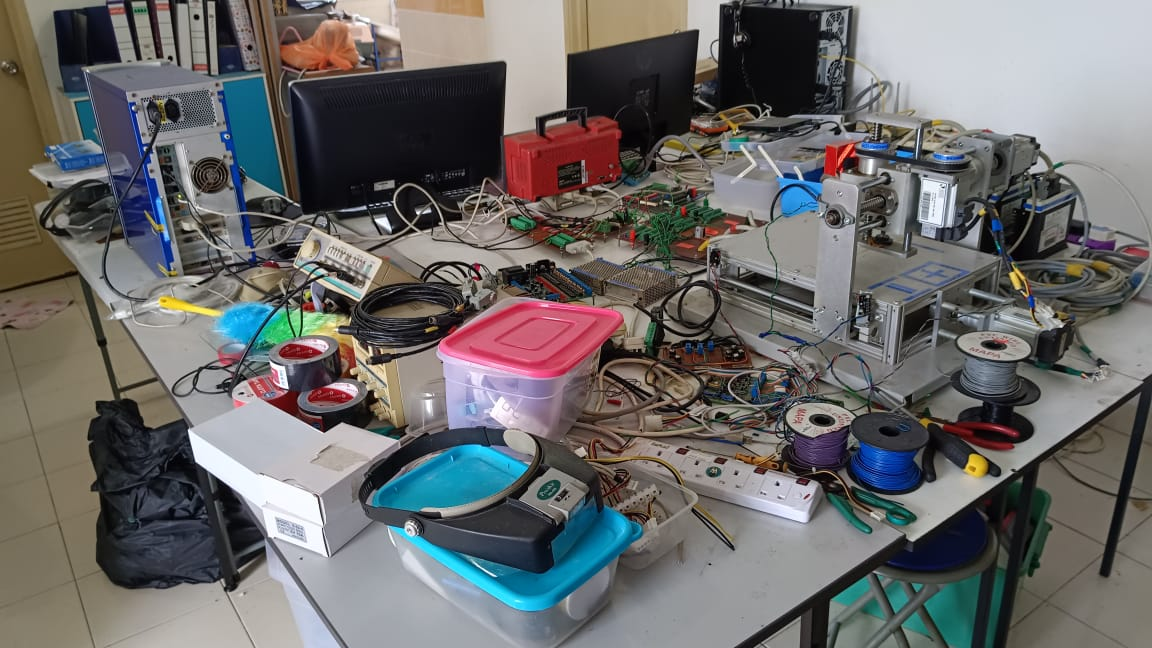
\includegraphics[width=1.60\textwidth]{Image0/THE-BACK-END-WhatsAppImage.jpeg} 
%%		\label{THE-BACK-END-WhatsAppImage.jpeg}
%%	\end{figure}
%% \end{landscape}


%% ==============================
\clearpage
\pagebreak

\begin{figure}
	\caption{Overview CNC system menvironment}
	\label{Overview-CNC-system-environment.pdf}
	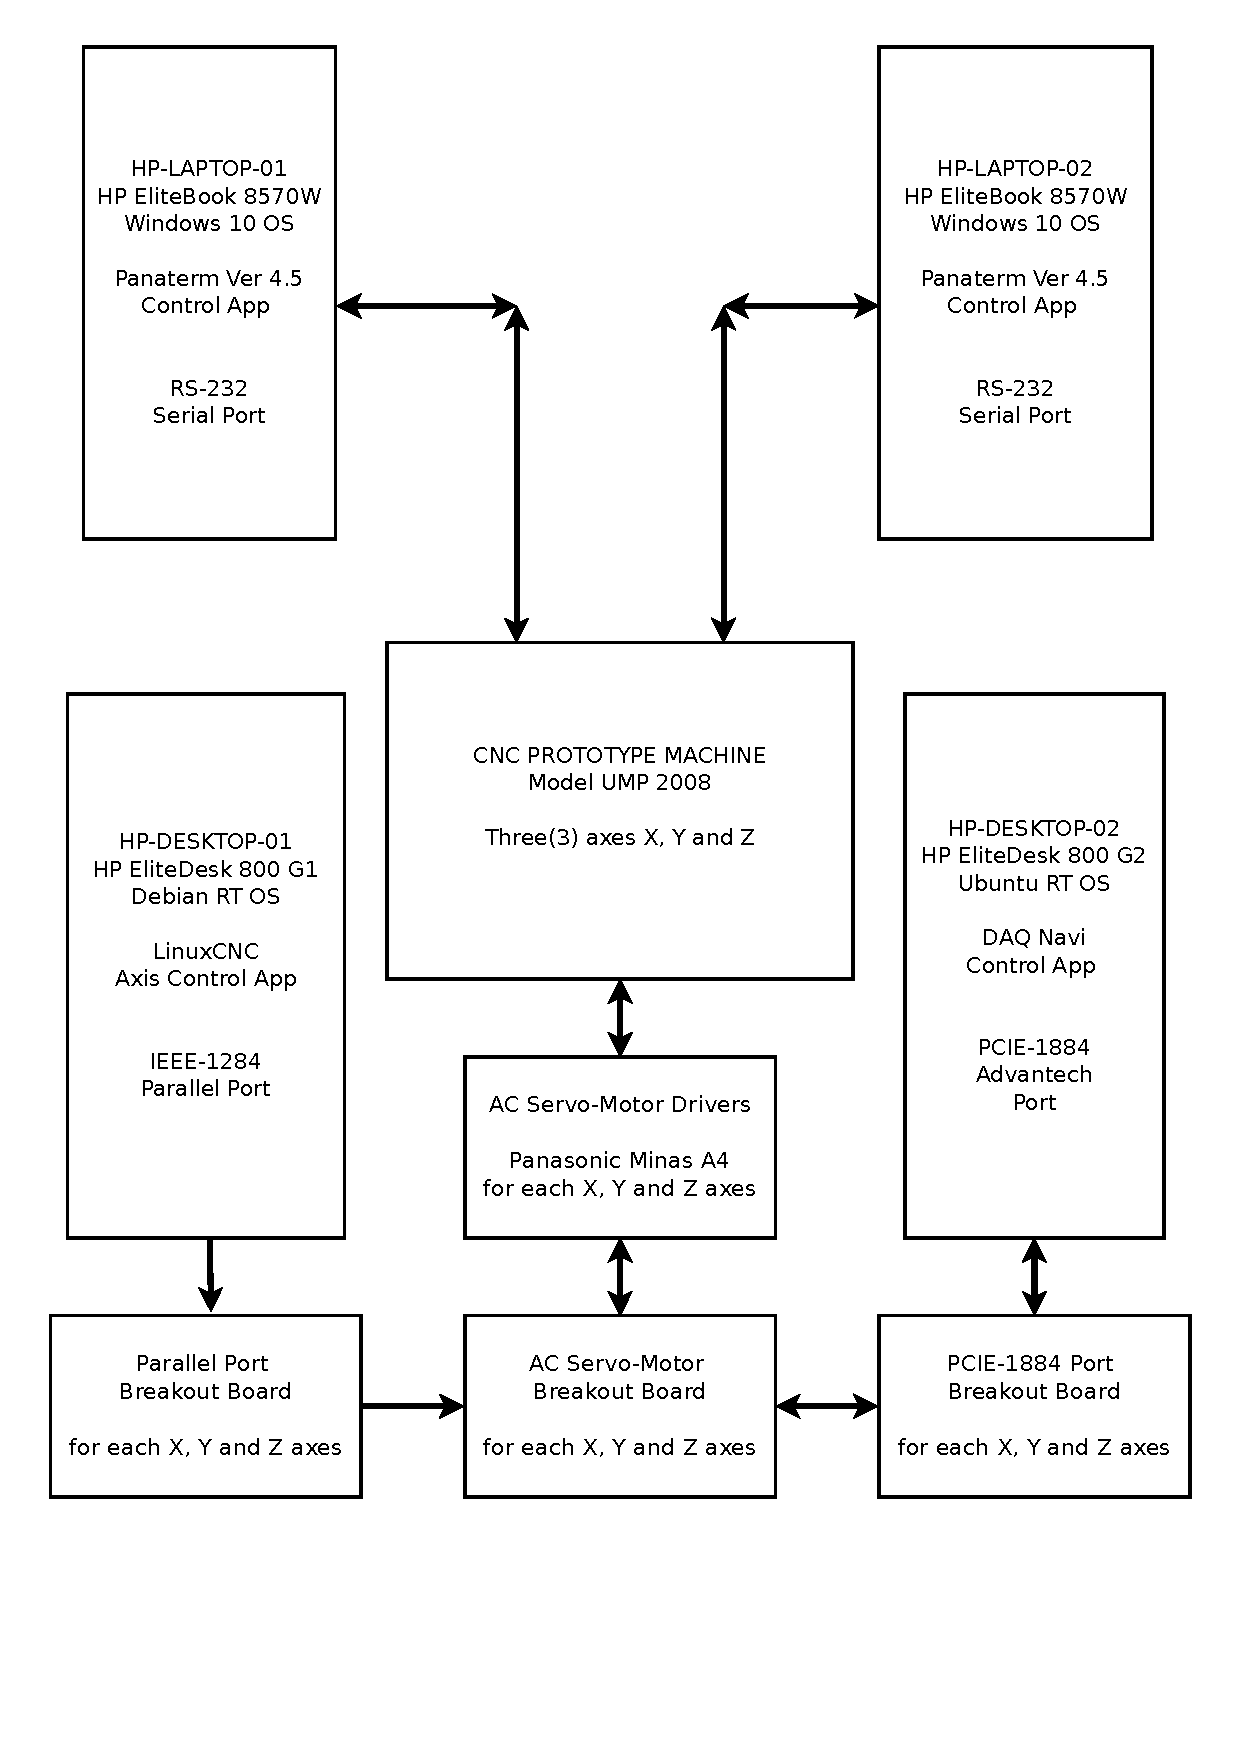
\includegraphics[width=1.00\textwidth]{Chap3/work-setup/Overview-CNC-system-environment.pdf} 
\end{figure}


\begin{figure}
	\caption{CNC-system-Panaterm-controller}
	\label{CNC-system-Panaterm-controller.pdf}
	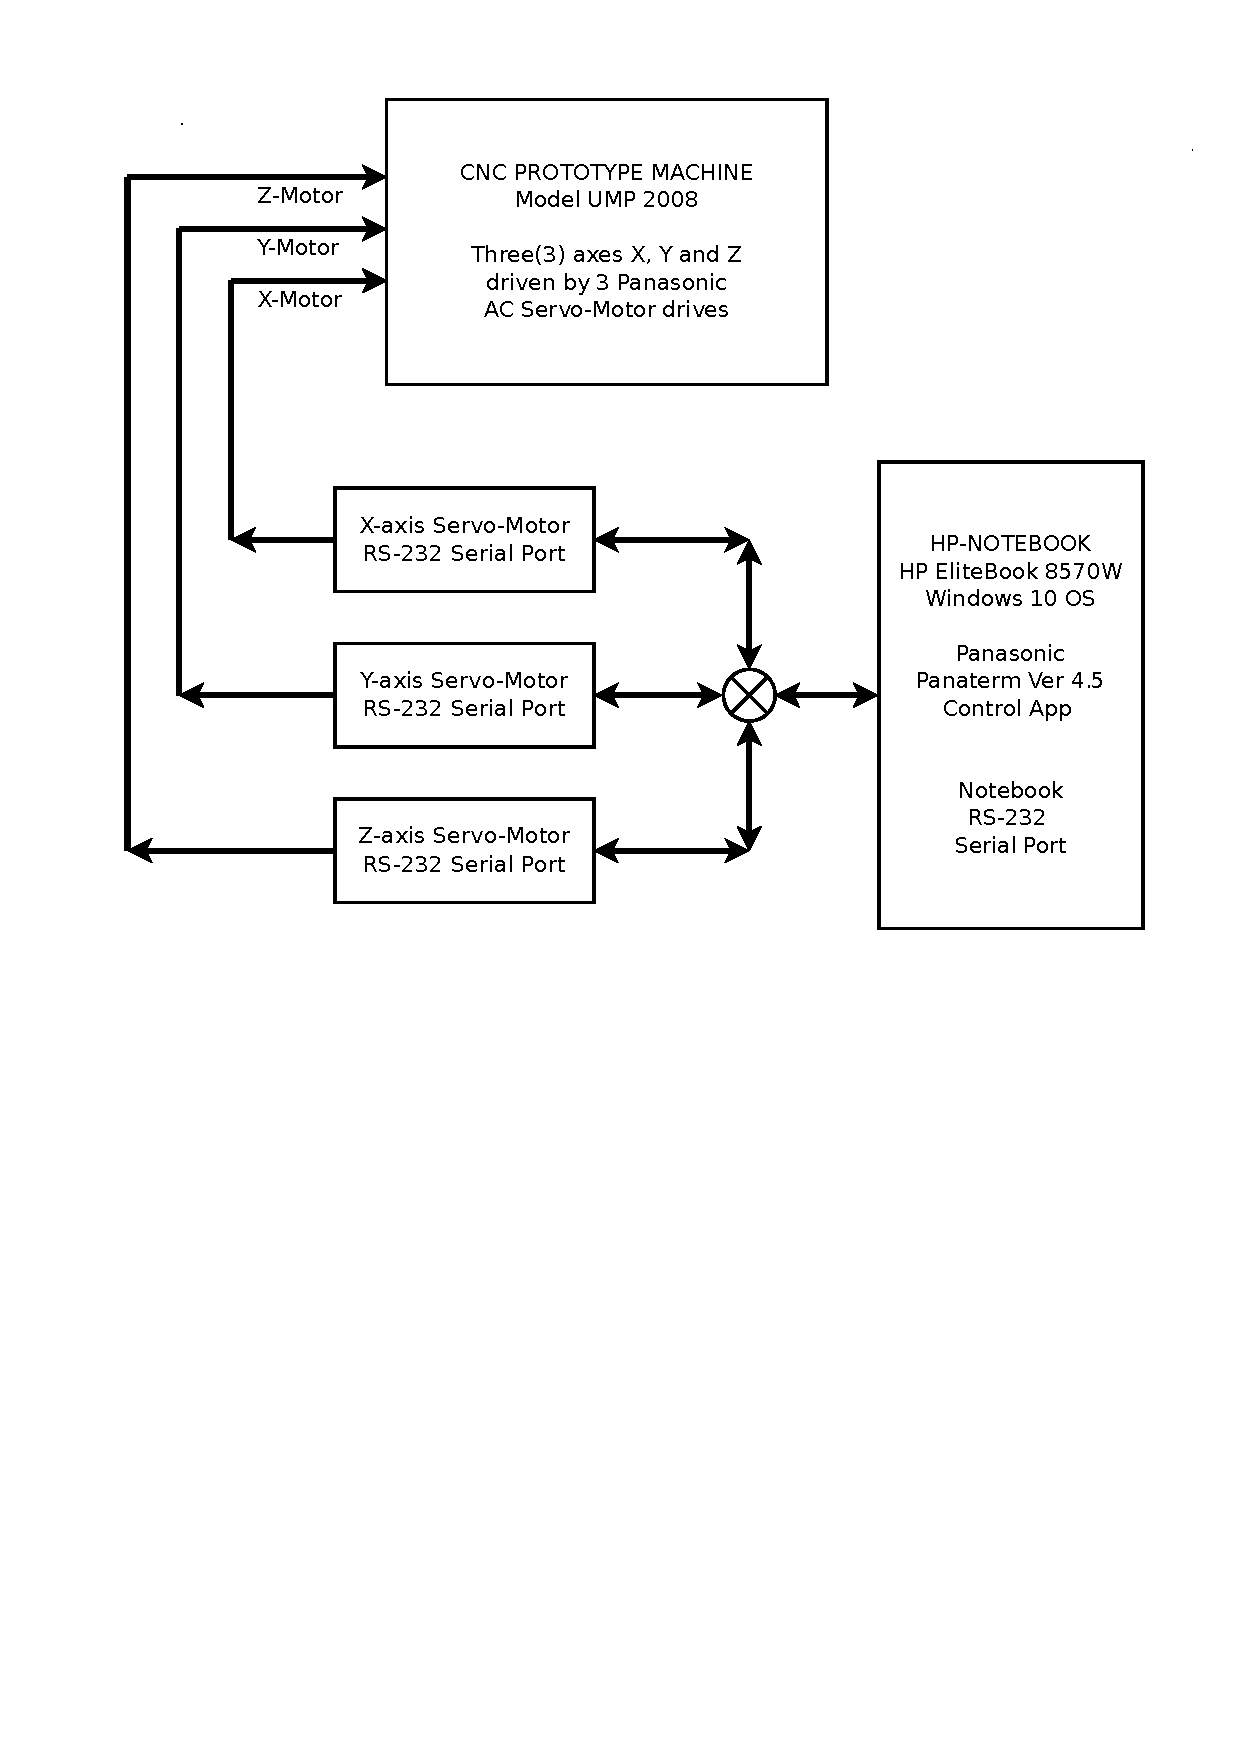
\includegraphics[width=1.00\textwidth]{Chap3/work-setup/CNC-system-Panaterm-controller.pdf} 
\end{figure}


\begin{figure}
	\caption{Parport-CNC-servo-PCIE-1884-wiring-diagram}
	\label{Parport-CNC-servo-PCIE-1884-wiring-diagram.pdf}
	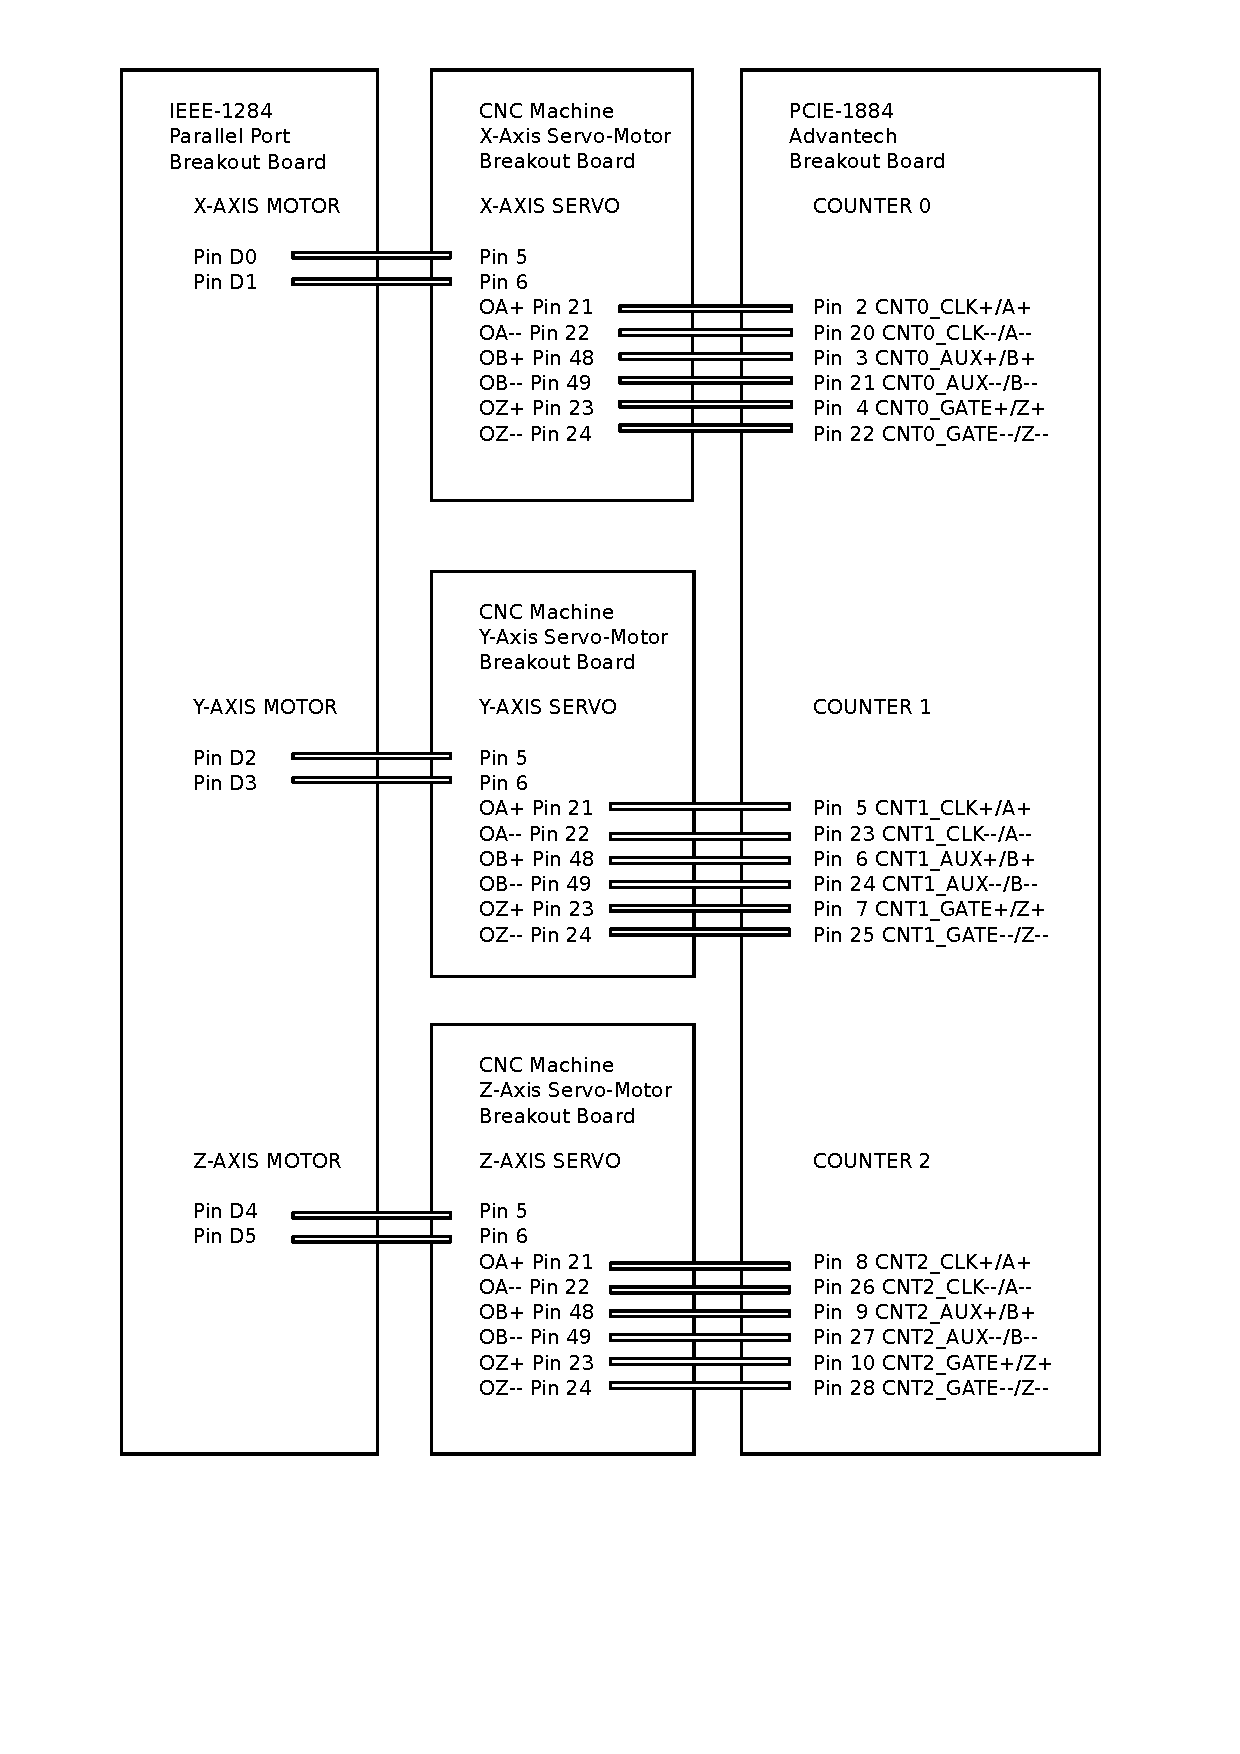
\includegraphics[width=1.00\textwidth]{Chap3/work-setup/Parport-CNC-servo-PCIE-1884-wiring-diagram.pdf} 
\end{figure}

\begin{figure}
	\caption{RS232 Snooper Circuit}
	\label{RS232-Snooper-Circuit.pdf}
	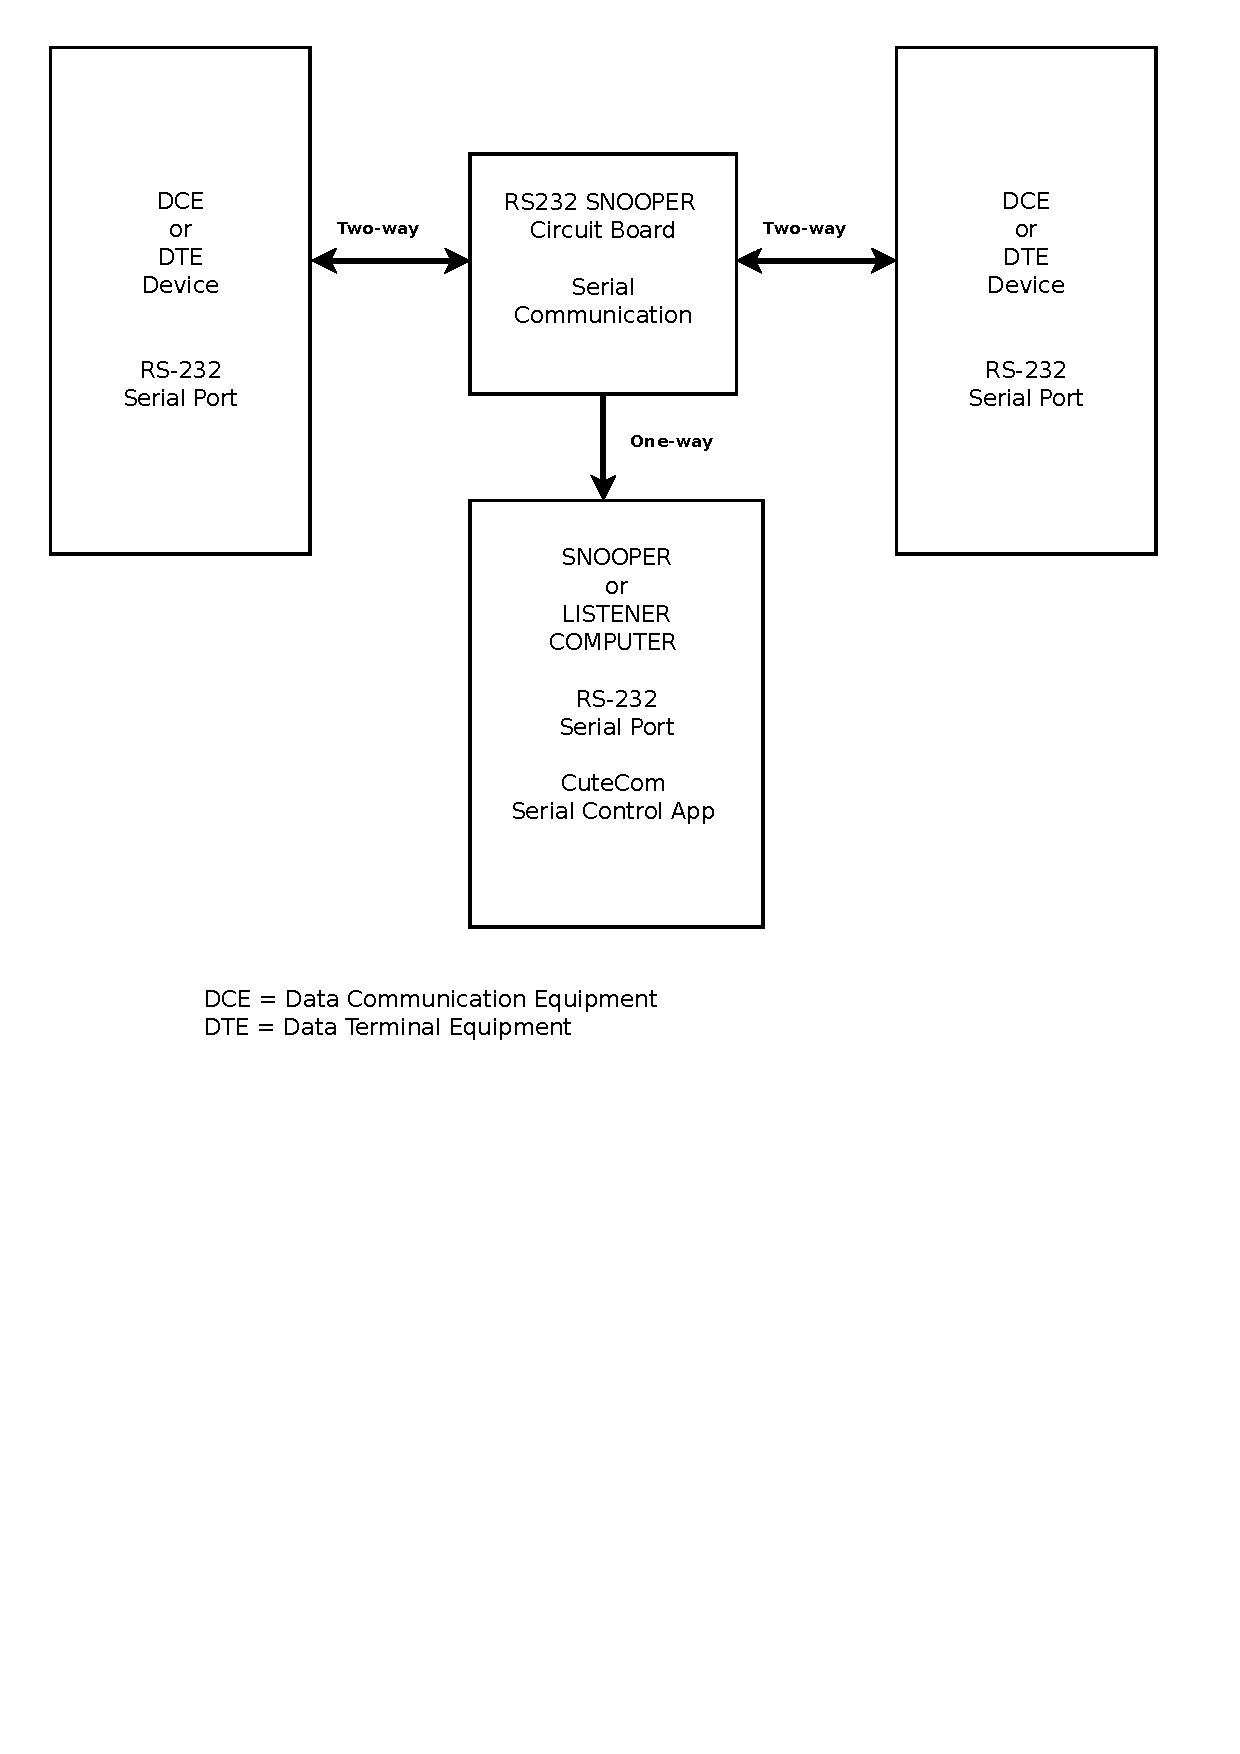
\includegraphics[width=1.00\textwidth]{Chap3/work-setup/RS232-Snooper-Circuit.pdf} 
\end{figure}


%%% ==============================
%%% END METHODOLOGY CHAPTER
